% !TeX encoding = UTF-8
% !TeX program = pdflatex
% !TeX spellcheck = it_IT

\documentclass[LaM,binding=0.6cm]{../sapthesis}
\usepackage{booktabs}
\usepackage{tabularx}
\usepackage{microtype}
\usepackage[italian]{babel}
\usepackage[utf8]{inputenc}
%\input{ix-utf8enc.dfu}
\usepackage{mathtools}
\usepackage{hyperref}
\usepackage{fancyvrb}


\hypersetup{pdftitle={Esempio d'uso della classe Sapthesis per una tesi di Laurea Magistrale},pdfauthor={Manuel Bannella}}

% Remove in a normal thesis
\usepackage{lipsum}
\usepackage{curve2e}
\definecolor{gray}{gray}{0.4}
\newcommand{\bs}{\textbackslash}


% Commands for the titlepage
\title{Progettazione e sviluppo di un sistema per la verifica
dell’integrità hardware e
firmware di un picosatellite}
\author{Manuel Bannella}
\IDnumber{1619174}
\course{Ingegneria Elettronica}
\courseorganizer{Facoltà di Ingegneria dell'informazione,
informatica e statistica}
\AcademicYear{2020/2021}
\copyyear{2021}
\advisor{Prof. Mauro Olivieri}
\advisor{Prof. Augusto Nascetti}


\authoremail{bannella.1619174@studenti.uniroma1.com}

\examdate{26 Ottobre 2021}
\examiner{Prof. Nome Cognome}
\examiner{Prof. Nome Cognome}
\examiner{Dr. Nome Cognome}
\versiondate{\today}

\DeclarePairedDelimiter\floor{\lfloor}{\rfloor}


\usepackage{listings}
\usepackage{color}

\definecolor{mygreen}{rgb}{0,0.6,0}
\definecolor{mygray}{rgb}{0.5,0.5,0.5}
\definecolor{mymauve}{rgb}{0.58,0,0.82}

\lstset{ %
  backgroundcolor=\color{white},   % choose the background color
  basicstyle=\footnotesize,        % size of fonts used for the code
  breaklines=true,                 % automatic line breaking only at whitespace
  captionpos=b,                    % sets the caption-position to bottom
  commentstyle=\color{mygreen},    % comment style
  escapeinside={\%*}{*)},          % if you want to add LaTeX within your code
  keywordstyle=\color{blue},       % keyword style
  stringstyle=\color{mymauve},     % string literal style
}



\begin{document}

\frontmatter

\maketitle

\dedication{Dedicato a\\ Francesco Savi}

\begin{abstract}

    %Illustrare il titolo della tesi: la prima funzione di un abstract è quella di spiegare il titolo della tesi e la correlazione con l’argomento scelto;
    %Sintetizzare gli aspetti importanti: che si tratti di un abstract tesi compilativa o di ricerca, triennale o magistrale, lo scopo fondamentale di questo strumento è di fornire informazioni sulla tesi anche a chi non ha tempo di leggerla per intero;
    %Offrire una visione completa della tesi: l’abstract è utile anche per fornire una prima panoramica del tuo elaborato al lettore, illustrando i punti trattati nel corpo della tesi;
    %Spiegare la metodologia e l’approccio scientifico alla materia: è importante, in una tesi, illustrare accuratamente la metodologia di lavoro adottata e il perché della scelta di un determinato approccio.
    %Tieni in considerazione anche che un buon abstract non è più lungo del 5 per cento dell’intera tesi triennale o magistrale: si tratterà, dunque, di scrivere circa 250 – 300 parole.

Questo lavoro di tesi magistrale si propone di sviluppare un sistema di controllo della consistenza dei dati di un "Sistema Embedded"\footnote{Sistema Embedded: sistema spesso parte integrante di sistemi più grandi progettato per svolgere un compito preciso e determinato (a differenza di quanto succede nei sistemi general purpose)} ed in particolare cerca di risolvere problemi relativi alla "reliability" di computer di bordo dedicato ad applicazioni aerospaziali.

Grazie allo sviluppo tecnologico raggiunto negli ultimi decenni ed in particolare in ambito dell'elettronica digitale, anche applicazioni specifiche di ambito aerospaziale come ad esempio lo sviluppo firmware di "Picosatelliti"\footnote{Picosatellite: i picosatelliti o picosat sono satelliti miniaturizzati insolitamente piccoli e leggeri, con una massa compresa tra 100 grammi e 1 kg} ha potuto beneficiare dell'aumento delle prestazioni e del rimpicciolimento dei singoli componenti hardware. 

Come conseguenza anche sistemi a risorse limitate hanno potuto sviluppare applicazioni firmware sempre più complesse e raffinate.

L'ambiente spaziale ed in particolare zone del cosmo come le fasce di Van Allen rappresenta però una sfida per quanto riguarda problemi di consistenza della memoria dell'intero sistema. Le radiazioni cosmiche possono infatti generare corruzioni all'interno del firmware.

In questo lavoro sono state usate diverse tecniche software con l'obiettivo di rilevare e correggere eventuali errori e malfunzionamenti del sistema hardware: - utilizzo di ridondanza software (di copie dello stesso firmware), - protezione dell'informazione tramite algoritmi di rilevazione e correzione dell'errore, - diagnostica ed eventuale esclusione dei sottosistemi non correttamente funzionanti.

L'approccio utilizzato durante l'implementazione di ogni singola tecnica ha cercato di rispettare gli standard di programmazione utilizzati per questi ambiti specifici (in particolare lo standard "Misra C"\footnote{Misra C :  standard di buona programmazione per software che richiedono un grado di affidabilità superiore rispetto alle applicazioni generiche} )
ed inoltre ogni nuovo sviluppo ha superato una serie di test di valutazione delle prestazioni che di rispetto dei requisiti richiesti da questi tipi di applicazioni.

I risultati ottenuti durante la fase di testing dei diversi applicativi hanno determinato un sensibile irrobustimento di tutto il firmware. Sebbene non sia stato possibile determinare sul microcontrollore i fattori come il consumo di memoria e di tempo, data l'impossibilità di simulare una situazione reale di volo, l'architettura software è stato resa il più possibile scalabile in modo da determinare un compromesso tra i fattori precedentemente espressi e la protezione del sistema.
\end{abstract}

\begin{acknowledgments}
DA COMPLETARE
Ho deciso di scrivere i ringraziamenti in italiano
per dimostrare la mia gratitudine verso i membri
del GuIT, il Gruppo Utilizzatori Italiani di \TeX, e, in particolare,
verso il prof. Enrico Gregorio.
\end{acknowledgments}

\tableofcontents

\listoffigures

\listoftables

% Do not use the starred version of the chapter command!
\chapter{Introduzione}
Nell' ottobre 2020, tramite il professor Mauro Olivieri sono riuscito a discutere con il professor Augusto Nascetti riguardo a possibili tesi magistrali per il corso di Ingegneria Elettronica. 

La mia intenzione di approfondire le conoscenze riguardo la scrittura di firmware per sistemi digitali Embedded calzava a pennello con uno degli sviluppi che il professore, in quel periodo, coordinava nel suo laboratorio sito nella sede di Ingegneria Aerospaziale in via Salaria. Lo sviluppo riguardava per l'appunto un \textbf{picosatellite} chiamato  \textbf{"CubeSat"}, ovvero ovvero un satellite di dimensioni ridotte composto da una parte meccanica che elettronica già precedente utilizzato e sviluppato dallo stesso laboratorio. 

Il progetto aveva l'obiettivo di eseguire una serie di esperimenti nel periodo di viaggio del satellite attorno all'orbita Terrestre. L'obiettivo era quello di raccogliere ciclicamente dati di natura chimica. La parte di firmware dedita a questo obiettivo era già stata sviluppata all'interno del codice fornito dal professore. 

Il mio obiettivo era diverso e riguardava principalmente l'attività di preservazione della consistenza dei dati del computer di bordo, poiché il satellite in questo caso doveva attraversare le cosiddette \textbf{"Fasce di Van Allen"}, una regione di spazio lontano dalla Terra (con un' altitudine compresa tra il migliaio di chilometri fino un limite esterno che supera i 40.000 km rispetto alla Terra), dunque una zona di cosmo molto diversa rispetto alle missioni precedenti poiché la quantità di radiazioni presenti era notevolmente superiori ad altre zone di spazio. 

Queste fasce possono essere rappresentate essenzialmente come un toroide di particelle cariche site all'interno della magnetosfera terrestre e le radiazioni sono trattenute per effetto della \textbf{"forza di Lorentz"}. 

Il problema principale di questa missione rispetto alle precedenti riguardava la consistenza della informazioni presenti nella memoria del satellite, la quale veniva perturbata dall'effetto sull'hardware dell'energia cinetica intrappolata da questa fascia. Poiché il satellite seguiva una traiettoria attorno alla Terra che gli permetteva di uscire e rientrare in queste fasce, il problema era periodico.

L'obiettivo del nostro lavoro di tesi è stato dunque la scrittura di una parte di firmware capace di mantenere una struttura codice e dati il più protetta possibile da eventuali corruzioni. Questa necessità ha portato alla definizione di una procedura di tolleranza di corruzioni/malfunzionamenti necessaria per il mantenimento delle funzioni del satellite per un periodo di tempo più lungo possibile. 

Per fare ciò la prima parte dell'attività di tesi ha riguardato un periodo di studio dello stato dell'arte dei sistemi elettronici, con particolare attenzione all'ambito delle problematiche di \textbf{"reliability"}, ovvero la probabilità che un sistema esegua con successo le azioni per cui è stato progettato per un periodo di tempo definito a priori. Questa caratteristica dei sistemi elettronici ha un'importanza particolare nell'ambito sia di applicazioni aerospaziali, di quelle navali ma anche in ambito spaziale: tutti questi ambiti richiedono come caratteristica principale sistemi il più possibile sicuri e capaci di rispondere ad eventuali guasti e malfunzionamenti.

La scrittura del firmware ha cercato di rispettare nel modo più appropriato possibile le regole di \textbf{Misra C}, ovvero delle regole di corretta scrittura di codice definiti per questi ambiti e che fanno riferimento a strutture di codice solide e facili da essere lette e "debuggate" (testate e corrette) anche da altre persone. Questa caratteristica è necessaria nei settori in cui l'attività di testing del codice è spesso eseguita da personale esterno rispetto a quello che scrive il firmware, in modo da garantire imparzialità nella validazione del codice eseguito e dunque una maggiore affidabilità dello stesso.
    
L'elaborato prodotto durante l'attività di tesi di laurea è volutamente strutturato in maniera da approfondire singolarmente ogni ambito di ricerca sviluppato e/o testato durante il periodo Ottobre 2020/Maggio 2021.
Ogni capitolo dunque affronta una parte dello sviluppo che poi infine viene integrato nel cosiddetto \textbf{"main"} del codice, ovvero la funzione principale che il satellite esegue continuamente durante il suo funzionamento e che attiva le applicazioni richieste.
    
La struttura di ogni capitolo di compone dunque delle seguenti sottosezioni:
\begin{itemize}
    \item spiegazione del problema da risolvere;
    \item ricerca di possibili implementazioni e scelta delle più appropriate da poi implementare, eseguendo se possibile un confronto di prestazioni tra i diversi algoritmi;
    \item spiegazione passo passo del codice C;
    \item test in modalità di debug utilizzando quando possibile direttamente l'hardware del codice descritto con valutazione dei risultati;
    \end{itemize}
    
In conclusione, il lavoro di tesi ha portato dei notevoli miglioramenti al firmware di bordo del satellite CubeSat. Le parti più importanti della memoria del sistema Abacus sono protette con una buona probabilità dalle radiazioni attraverso un sistema di risoluzione dei malfunzionamenti. Anche in caso di malfunzionamenti, il sistema tende a limitare la frequenza dei reset che il sistema esegue in modo da garantire un utilizzo del satellite il più lunga possibile. 

L'architettura del codice inserito all'interno del firmware ha tenuto dunque conto del compromesso tra robustezza di codice e dati del microcontrollore e \textbf{carico della nuova parte di codice } su tutto il firmware. Un occupazione temporale troppo prolungata dell'attività di protezione e recupero dell'informazione avrebbe limitato l'attività di sperimentazione.



\mainmatter

\chapter{Microcontrollori}

Un \textbf{microcontrollore} (MCU, MicroController Unit) è un single-chip computer, ovvero un microcalcolatore integrato su un singolo chip. Come suggerisce il nome, il microcontrollore è utilizzato principalmente per realizzare sistemi di controllo digitale e, in particolare, nei dispositivi cosiddetti "Embedded".

Per sistemi \textbf{Embedded} facciamo riferimento a sistemi elettronici di elaborazione a microprocessore progettati appositamente per una determinata applicazione "special purpose" (ovvero non riprogrammabili dall'utente per altri scopi), spesso con una piattaforma hardware ad hoc, integrati nel sistema che controllano e in grado di gestirne tutte o parte delle funzionalità richieste.

\section{Caratteristiche del sistema hardware MCU/FPGA MSP430}

La famiglia \textbf{MSP430} è una famiglia di microcontrollori \textbf{ultralow-power} (a basso consumo di potenza) prodotta da textbf{Texas Instruments}. 
La caratteristica principale è per l'appunto il risparmio di potenza consumata, poiché tutti i modelli prodotti dispongono di un \textbf{DCO} ("Digital Controlled Oscillator"), un'unità che permette il risveglio in modalità attiva dalla modalità definita come low-power mode con tempi dell'ordine dei microsecondi. 
Questo meccanismo di elaborazione inframezzato da periodi di inattività e attesa permette di razionare il consumo di potenza media.

L'architettura del microcontrollore usato per questa tesi, ovvero l' MSP430F5438A, consiste in una CPU ad architettura \textbf{RISC} ("Reduced Instruction Set Architecture") a 16 bit, 16 registri a 16 bit in cui possiamo evidenziare un registro chiamato "\textbf{Constant Generator}", un registro dedicato all'efficienza massima di codice. In esso infatti vengono immagazzinate delle costanti che possono essere utilizzate senza essere immagazzinate in memoria centrale, permettendo dunque di sostituire particolari istruzioni (come ad esempio l'incremento ad uno di un registro) e di limitare quindi la libreria di istruzioni che l'architettura utilizza.

La serie MSP430x sono inoltre microcontrollori configurati con 3 diversi timer a 16 bit, un analog-to-digital (A/D) converter a 12 bit, fino a quattro interfacce di comunicazione "USCI", ("Universal serial communication interfaces"), un moltiplicatore hardware, DMA ("Direct memory access") e fino a 87 pin di I/O.

Di seguito nella figura 1.1, è possibile consultare il documento di informazioni presente nel datasheet dedicato per sistemi MSP430xx:

    \begin{figure}[htbp]
    \centerline{
\includegraphics[scale=.67]{examples/Msp430Datasheet.PNG}}
    \caption{Datasheet del microcontrollori della famiglia MSP430F543xA e MSP430F541xA}
    \label{fig}
    \end{figure}
Datasheet del microcontrollori della famiglia MSP430F543xA e MSP430F541xA
\clearpage

\section{ Architettura del satellite Cubesat }

Il sistema \textbf{Abacus} (nel nostro caso abbiamo utilizzato la versione 2017) è un'unità \textbf{On-board computer} con una piattaforma hardware general purpose, adatta per un'ampia
gamma di missioni satellitari. È progettato per essere flessibile e scalabile in termini di consumi di
potenza. 

È composto da due core diversi, un \textbf{MCU} ("Microcontrollore", l'MSP430F5438A) e un \textbf{FPGA} ("Field Programmable Gate Array", chiamata Spartan-3E ) che lavorano in modo cooperativo alla gestione delle funzioni di volo e di elaborazione dell'intero satellite.

Il design del sistema offre la possibilità di riconfigurare il codice FPGA e il firmware dell'MCU direttamente in volo sia tramite un sistema automatizzato, attraverso un codice di bootloader scritto all'interno del codice, sia esternamente, attraverso una comunicazione radio con la stazione base, ovvero dall'operatore.

    \begin{figure}[htbp]
    \centerline{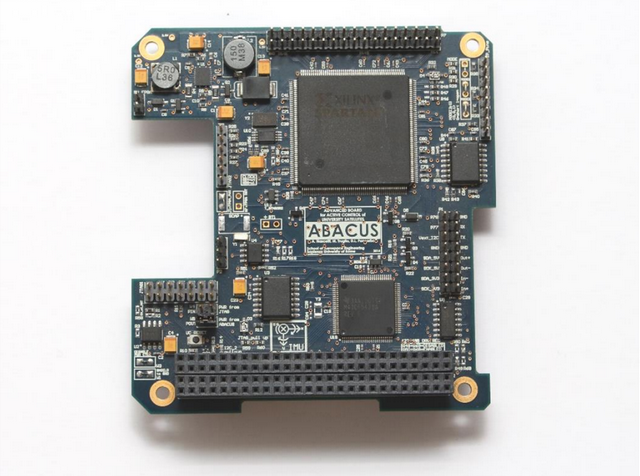
\includegraphics[scale=.67]{examples/AbacusImage.PNG}}
    \caption{Foto del sistema Abacus in cui è possibile apprezzare l'MCU MSP430F5438A e la FPGA Spartan-3E}
    \label{fig}
    \end{figure}
    \clearpage
    
Queste sono le principali caratteristiche del sistema Abacus:
\begin{itemize}
    \item \textbf{Due core} (MCU MSP430 e FPGA Spartan-3E) direttamente interconnessi attraverso con un textbf{bus a 24 linee};
    
    \item \textbf{Un Microcontrollore} (MSP430) con architettura \textbf{RISC} a 16 bit, con un clock cha arriva fino a \textbf{25 MHz};
    
    \item \textbf{10 ingressi analogici} da 3,3V e fino a 45 canali GPIO digitali;
    
    \item \textbf{16 GPIO} modificabili a livello di tensione con funzionalità di interruzione;
    
    \item 4 x porte \textbf{COM} (di cui una anche nei livelli standard RS 422/485 Full o Half Duplex), 2 x \textbf{$I^2C$} e 1 x \textbf{SPI};
    
    \item \textbf{FPGA} funzionante a 25 MHz o 100 MHz (predefinito);
    https://www.overleaf.com/project/6006a99f6967e0c12b852024
    \item Embedded \textbf{IMU} ("Inertial measurement unit") con \textbf{magnetometro},\newline \textbf{accelerometro} e \textbf{giroscopio} tutti triassiali;
    
    \item Sensori incorporati: 3 x \textbf{sensori di temperatura}, 1 x \textbf{monitor di corrente assorbita}, 1 Embedded \textbf{RTC} ("Real Time Clock");
\end{itemize}

    \begin{figure}[htbp]
    \centerline{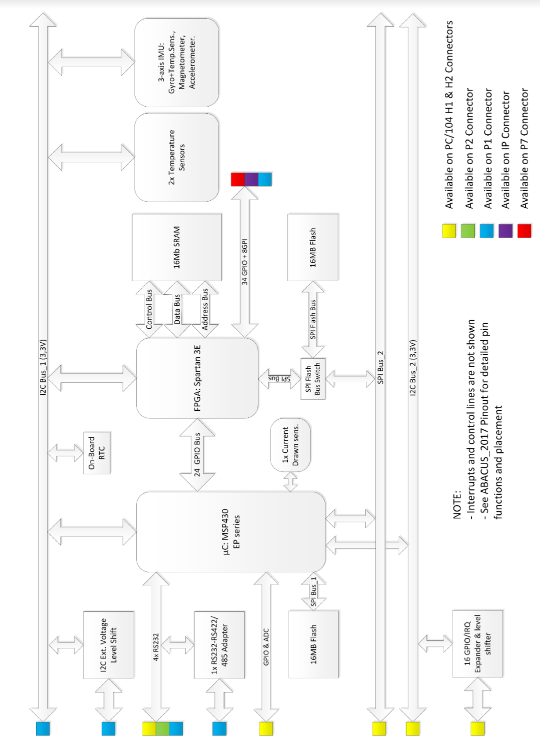
\includegraphics[scale=.8]{examples/AbacusDiagram.PNG}}
    \caption{Diagramma delle interconnessioni hardware in Abacus}
    \label{fig}
    \end{figure}
\clearpage
\chapter{Fault Tolerance}
Nell'ingegneria dell'affidabilità la tolleranza ai guasti (o "\textbf{fault-tolerance}", dall'inglese) è la capacità di un sistema di non subire avarie (cioè interruzioni di servizio) anche in presenza di guasti. La tolleranza ai guasti è uno degli aspetti che costituiscono l'\textbf{affidabilità}. È importante notare che la tolleranza ai guasti non garantisce l'immunità da tutti i guasti, ma solo che i guasti per cui è stata progettata una protezione non causino fallimenti.

Questo concetto è molto studiato in applicazione elettroniche di ambito spaziale principalmente per due motivi:
\begin{itemize}
    \item L'impossibilità in orbita della \textbf{riparazione} di parti software e hardware per un periodo di tempo molto lungo.
    
    \item La presenza di \textbf{radiazioni ionizzanti} che sono localizzate nelle "Fasce Di Van Allen" che possono portare il sistema elettronica e meccanico a guasti e/o rotture.
\end{itemize}

I controlli di protezione (che vengono effettuati a tempo di esecuzione), assieme a controlli analoghi effettuati staticamente (come a tempo di progettazione o di compilazione), sono una metodologia molto efficace per ottenere un'elevata robustezza (rapida rilevazione degli errori e loro confinamento) in un sistema. 

La tolleranza ai guasti può portare al peggioramento di altre prestazioni, per cui nella progettazione di un sistema è necessario trovare adeguate ottimizzazioni e compromessi. 

Nelle prossime sezioni verranno analizzate diverse tecniche sia di progettazione hardware che di programmazione software utilizzate per garantire che un sistema sia più affidabile e resiliente. Tutte queste tecniche portano il progettista essenzialmente a generare un sistema più ridondante, ovvero costituito da più parti rispetto al necessario, utilizzate col fine di sostituire o riparare durante il periodo di esecuzione del firmware eventuali parti danneggiate o rotte.

\section{Radiazione spaziale e gestione della corruzione dell'informazione}

Uno dei maggiori problemi nell'ambiente spaziale è la presenza di radiazioni cosmiche.
I raggi cosmici sono particelle energetiche provenienti dallo spazio esterno alle quali è esposta la Terra come qualunque altro corpo celeste, nonché i satelliti e gli astronauti in orbita spaziale.

La presenza di raggi cosmici è inoltre preponderante nelle orbite Terrestri poco al di sopra rispetto alla LEO ("Low Earth Orbit"), questo perché il campo magnetico Terrestre tende a bloccare le radiazioni provenienti dallo spazio, schermarle ed infine intrappolarle all'interno di una zona di spazio superiore alle LEO chiamate "Fasce di Van Allen".
A sua volta queste fasce sono divise in due diverse orbite (la prima fascia dai 1000 km ai 6000 km di distanza dalla Terra, la seconda da circa 6000 a 60000 km di distanza). La divisione è principalmente eseguita in base al tipo e all'intensità delle radiazioni di alta energia.

Le radiazioni intrappolate in queste fasce sono costituiti principalmente da:
\begin{itemize}
    \item brillamenti solari.
    
    \item raggi cosmici galattici.
    
    \item particelle intrappolate.
\end{itemize}

L'entità dell'energia dei raggi cosmici, come si può evincere dalla figura 2.1, è dell'ordine dei $MeV$ e può arrivare a $GeV$ (con misurazioni dell'ordine  dei $100 MeV$ - $10GeV$).
    \begin{figure}[htbp]
    \centerline{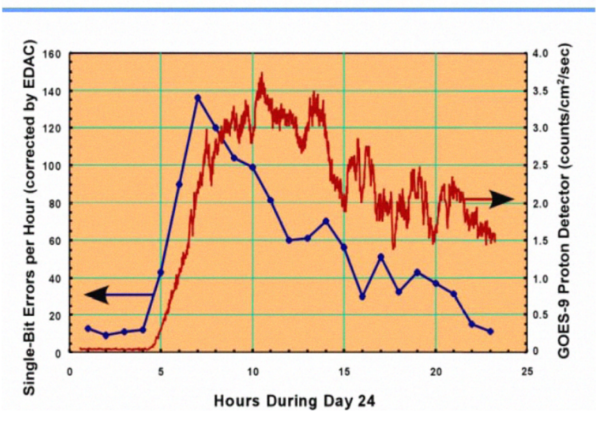
\includegraphics[scale=.67]{examples/CassiniFlares.PNG}}
    \caption{Entità della radiazione cosmica valutata durante dal satellite Cassini della Nasa.}
    \label{fig}
    \end{figure}
\clearpage
\section{ Ridondanza Hardware }

Per ridondanza Hardware si intende l'inserimento nell'architettura del sistema fisico di componenti aggiuntivi, ovvero dell'hardware suppletivo, in un sistema soggetto a malfunzionamenti al fine di contribuire all'integrità del sistema e quindi il mantenimento delle funzioni per cui è stato implementato.

La ridondanza Hardware è la forma generalmente più utilizzata e consiste essenzialmente nella replica di hardware di sistemi digitali già utilizzati nell'architettura base.

Un fattore importante che premia l'utilizzo di hardware è essenzialmente la scalabilità dei componenti e dunque progressiva diminuzione del loro costo. L'hardware ha infatti raggiunto delle grandezze così esigue da permettere l'integrazione di sempre più sottosistemi all'interno dello stesso circuito integrato mantenendo un costo sempre basso. Di conseguenza sempre meno materiale viene utilizzato per fornire la stessa funzione e il costo del singolo pezzo hardware è in continua discesa.

A riprova di ciò, possiamo valutare la ben nota "\textbf{legge di Moore}", figura 2.1 ovvero una proiezione sul numero di transistor all'interno dei chip per unità di grandezza in un determinato anno. La curva è in continua ascesa e finché lo sarà il prezzo dei singoli componenti scenderà di conseguenza.

    \begin{figure}[htbp]
    \centerline{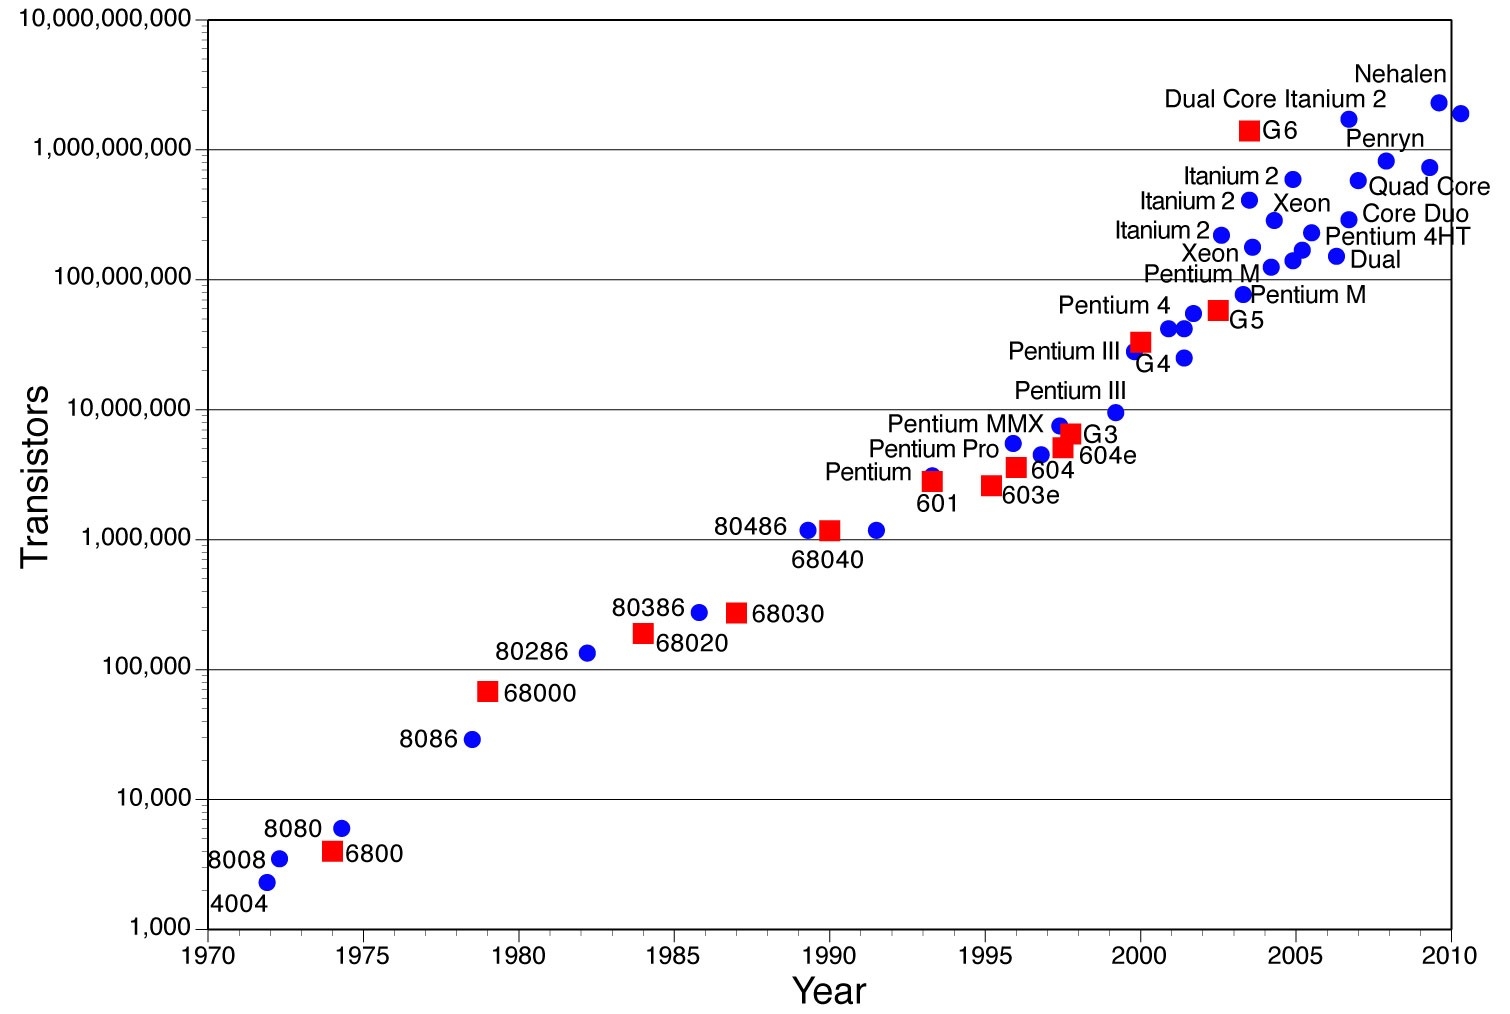
\includegraphics[scale=.27]{examples/Moores_Law.jpg}}
    \caption{Una rappresentazione grafica della legge di Moore in cui viene analizzato il numero di transistor presenti in un singolo processore.}
    \label{fig}
    \end{figure}
\newline

\subsection{Ridondanza Hardware Passiva}

Consiste nel mascheramento dell'occorrenza di malfunzionamenti attraverso la tecnica di "\textbf{Fault-masking}", la quale consiste nel nascondere l'avvenimento di guasti o mancato rilevamento di essi attraverso l'utilizzo di ridondanza hardware. 

Attraverso diverse tecniche è possibile dunque il comportamento della parte danneggiata.

\begin{itemize}
    \item "\textbf{Triple modular redundancy}": utilizza un sistema di voto in riferimento a tutti i diversi moduli che rappresentano l'uno una replica dell'altro. 
    
    Grazie al principio di maggioranza anche se uno dei moduli non è corretto, il comportamento rimane inalterato.
    
    \begin{figure}[htbp]
    \centerline{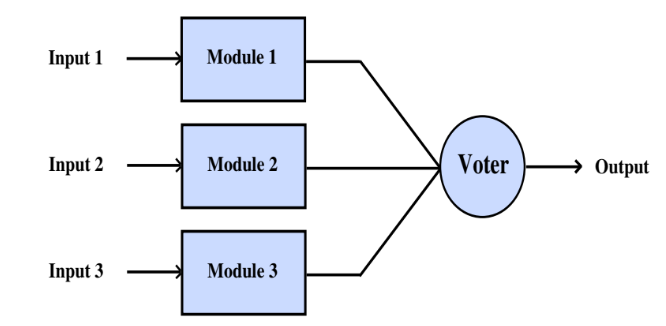
\includegraphics[scale=.67]{examples/TripleRedudancy.PNG}}
    \caption{Uno schema esplicativo della tecnica "Triple Modular Redudancy".}
    \label{fig}
    \end{figure}
\newline
    
    \item "\textbf{N-modular redundancy}": risulta una generalizzazione della tecnica precedente. Questo perché utilizzando la tecnica precedente è possibile "mascherare" il comportamento soltanto di uno dei tre moduli. Il concetto di N-modular è lo stesso del Triple Modular generalizzato a N identici dispositivi hardware che producono idealmente lo stesso output. In questo modo è possibile proteggere un numero di malfunzionamenti pari a $\floor*{\frac{N}{2}}-1$
    
    \begin{figure}[htbp]
    \centerline{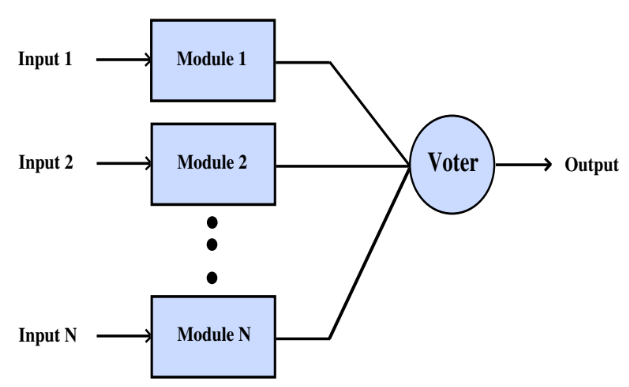
\includegraphics[scale=.67]{examples/NModularRedudancy.PNG}}
    \caption{Uno schema esplicativo della tecnica "N-modular Redudancy".}
    \label{fig}
    \end{figure}
\newline
\end{itemize}

\subsection{Ridondanza Hardware Attiva}

Consiste invece in una metodologia più articolata di ridondanza hardware e articolata principalmente in 3 fasi ("\textbf{Fault Detection}","\textbf{Fault Location"} e {"Fault recovery"}) e che nella sua totalità consiste nel monitorare un sistema, identificare quando si è verificato un guasto e individuare il tipo di guasto e la sua posizione ed infine la correzione dell'errore/malfunzionamento.

La ridondanza hardware attiva non maschera il malfunzionamento e tende invece a localizzare il punto del sistema hardware in cui è in atto il malfunzionamento. 

Una volta determinata la locazione del malfunzionamento, il sistema provvede dunque alla riconfigurazione dell'elemento e dunque alla risoluzione del problema.

I sistemi satellitari sono per l'appunto quelli che più utilizzano le tecniche di ridondanza hardware attiva al fine di garantire un corretto comportamento del sistema per il tempo maggiore possibile.

Di seguito analizziamo le principali tecniche utilizzate:

\begin{itemize}
    \item \textbf{Duplicazione con confronto}: il concetto di base della duplicazione con tecnica di confronto è quello di sviluppare due hardware
    moduli che possono svolgere contemporaneamente la stessa funzione e confrontare i propri
    uscite.
    
    Se le due uscite sono conformi l'una all'altra, l'uscita è corretta e può essere utilizzata una delle due ulteriormente. In caso di disaccordo, l'errore viene segnalato dal comparatore. Questa tecnica è
    utilizzato per il rilevamento degli errori.
    \begin{figure}[htbp]
    \centerline{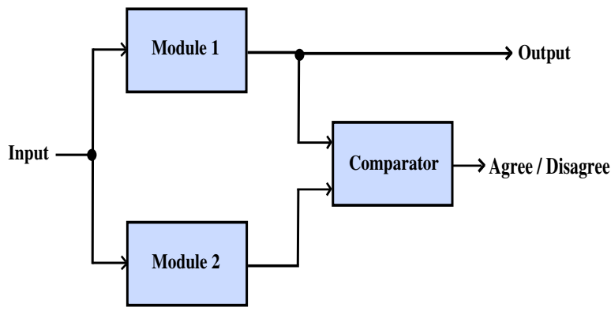
\includegraphics[scale=.67]{examples/ActiveComparator.PNG}}
    \caption{La sezione in codice C riguardante la definizione dei puntatori da cui iniziare a leggere i codici di backup.}
    \label{fig}
    \end{figure}
\newline
    
    \item \textbf{Standy Sparing}: in questa tecnica, un modulo è scelto come modulo "operativo" e uno o più moduli fungono da "pezzi di ricambio".
    
    Schemi di rilevamento dei guasti come quello sopra menzionato vengono utilizzati per rilevare il guasto nel sistema. Quindi viene determinata la posizione del guasto. 
    
    \item \textbf{Watchdog Timers}: si utilizza un timer hardware dedicato che deve essere ripristinato ripetutamente dal sistema. Se il sistema non riesce a ripristinare il timer, significa che condizione errata.
    
    In tal caso, il sistema stesso viene messo a ripristinare la condizione supponendo che
    inizierà dallo stato noto e privo di errori.
    
\end{itemize}
\section{ Ridondanza Software}
Gli schemi di "\textbf{Fault Tolerance}" già espressi in precedenza possono essere implementati in maniera analoga anche nel software.
Questo può essere fatto scrivendo una piccola routine che può controllare periodicamente lo stato della memoria
leggendo e scrivendo ripetutamente su di esso. 


Le principali tecniche di ridondanza software possono essere divise in queste categorie:
\begin{itemize}
    \item \textbf{Controlli di consistenza}: questo schema richiede una conoscenza anticipata delle informazioni che devono essere corrette. Ad esempio, nel contesto delle applicazioni spaziali, un parametro di un determinato sensore contenuto in uno dei sottosistemi non dovrebbe superare un determinato limiti, altrimenti ci sarebbe una compromissione dell'intera missione. Questo valore può essere memorizzato e la routine del software può controllare ripetutamente se il valore in tempo reale si trova all'interno intervallo definito o meno. In caso di superamento dei valori nominali, una flag può essere impostata per segnalare al sistema di eseguire l'azione appropriata.
    
    \item \textbf{Controlli delle "Funzioni del Software"}: questi controlli vengono eseguiti per verificare le capacità del sistema e il corretto funzionamento di moduli di sistema. Ad esempio, il processore può scrivere dei specifici "Test Cases" in memoria e
    leggerli al fine di determinare la corretta memorizzazione e recupero dei dati.

    \item \textbf{Replicazione del software}: il concetto di base è quello della programmazione di diverse versioni indipendenti di software.
    Le diverse versioni vengono tutte utilizzate e poi si arriva a confrontare i risultati di tutti gli algoritmi. Ciascuno di questi moduli è progettato e sviluppato da
    diversi gruppi di persone per garantire che non ci siano due gruppi che commettano lo stesso errore.

\end{itemize}

\section{Principali tecniche di ridondanza utilizzate nel progetto Abacus}

Dopo aver analizzato le principali metodologie di ridondanza sia hardware che software, andiamo ad esaminare ciò che è stato fatto nel lavoro di tesi ed in particolare sul microcontrollore MCU MSP430.
\newline
Per quanto riguarda l'implementazione di queste strategie di protezione da corruzioni e malfunzionamenti, la maggior parte dello sviluppo nel nostro caso  ha riguardato l'ampliamento della ridondanza software a sfavore di quella hardware.

La scelta è stata fatta principalmente per due motivi:
\begin{itemize}
    \item un limitato spazio fisico in cui inserire eventuali doppioni di parti hardware del sistema. L'inserimento di nuovi sottosistemi nel picosatellite avrebbe necessariamente richiesto una riprogettazione del sistema dal punto di vista elettronica, dal punto di vista meccanico e per quanto riguardo il consumo di potenza dell'intero satellite.
    \item l' occupazione di memoria (sia RAM in esecuzione che ROM) del microcontrollore è notevolmente inferiore rispetto allo spazio di memoria disponibile.
\end{itemize}
\newline
Lo sviluppo della Fault Tolerance ha dunque sfruttato molte delle tipologie di tecniche di ridondaza software già definite teoricamente in precedenza e 
l'implementazione ha principalmente riguardato:
\begin{itemize}
    \item Controlli di consistenza: è consistita principalmente nell'utilizzo di strutture dati a lunghezza fissa, generalmente delle strutture a array di dati a scapito di uno scarso utilizzo della parte di memoria definita "heap" (a lunghezza variabile) in modo da poter garantire in fase di esecuzione un controllo sulla dimensione dell'occupazione di memoria. Un'altra implementazione ha riguardato l'utilizzo di sezioni di memoria divise e distanti tra loro. La sua definizione è stata definita a priori (vedremo successivamente l'utilizzo di parti di memoria definite "persistent" all'interno della RAM ). Tale implementazione é di fatto la replicazione della strategia già espressa in precedenza sulla scala di sezioni di codice.
    \item Controlli di funzione: l'utilizzo di algoritmi di rivelazione di errori (ad esempio l'algoritmo CRC, "Cyclic Redudancy Check") atti a prevenire eventuali corruzioni generate dall'interazione del satellite con la radiazione spaziale.
    \item Replicazione del software: è consistita nella creazione e successivo inserimento di copie di codice di codice all'interno della memoria, utilizzabili secondo una logica di utilizzo da parte del microcontrollore tramite un algoritmo definito di "Bootloader". La replicazione ha riguardato anche la replicazione sia in memoria RAM che ROM di alcune sezioni di dati importanti immagazzinati durante la missione, come ad esempio le informazioni riguardanti lo stato del satellite.
\end{itemize}

\chapter{Bootloader}

\section{Cos'è un bootloader?}

L'algoritmo di \textbf{bootloader} è una parte di codice collocata nella parte iniziale del programma che permette di programmare o aggiornare la memoria flash del microcontrollore “MSP430” della Texas Instruments.

Questa funzionalità può essere attivata tramite degli apposite istruzioni fornite al microcontrollore tramite diversi protocolli di comunicazione come ad esempio tramite il protocollo seriale UART. 
Il Bootloader permette dunque all’utente il controllo delle attività del microcontrollore in tempo di esecuzione (sia per quanto riguarda il codice eseguito che i dati che il microcontrollore mantiene) e permette dunque un controllo mediato da una parte specifica del codice o addirittura da un altro dispositivo esterno (ad esempio un altro computer o un FPGA).

La parte di codice che esegue la funzionalità di sovrascrittura della memoria, spesso chiamata  \textbf{"Bootstrap Loader"},  \textbf{"Bootstrap"} o  \textbf{"Boot Loader"}, è un codice apposito alla scrittura delle nuove istruzioni comunicate e deve essere necessariamente mantenuta integro, poiché essendo il primo programma richiamato in fase di inizializzazione, bloccherebbe inevitabilmente le funzionalità dell'MCU. Il codice di Bootloader dunque viene collocato in una zona di memoria sicura e protetta e che non permette una sua involontaria o errata scrittura. Anche la lettura di questa zona di memoria è protetta da un'apposita password in modo da garantire la lettura diretta o indiretta soltanto se voluto.

Per invocare il bootloader, la sequenza di ingresso nel codice di Bootloader deve essere applicata ad un pin dedicato. Dopo fatto ciò, un carattere di sincronizzazione, seguito dal data frame per il comando specifico garantisce l’inizio dell’attività di sovrascrittura della memoria.


\subsection{Principali utilizzi della funzionalità di Bootloader all'interno dei microprocessori}
L'utilizzo più comune per quanto riguarda i microcontrollori è quello di scrivere su di esso una particolare funzione o porzione di codice all'interno della memoria Flash in tempo reale.
Questo evento viene generato generalmente nel momento in cui avviene un software reset del dispositivo è dunque possibile scegliere tramite il bootstrap di eseguire il vecchio codice già scritto sulla memoria non volatile del microcontrollore oppure di trasferire un nuovo programma e sovrascrivere in questo modo la memoria Flash. In questo modo è possibile eseguire e testare diverse versioni di codice semplicemente portando in fase di inizializzazione il microcontrollore.

\begin{figure}[htbp]
\centerline{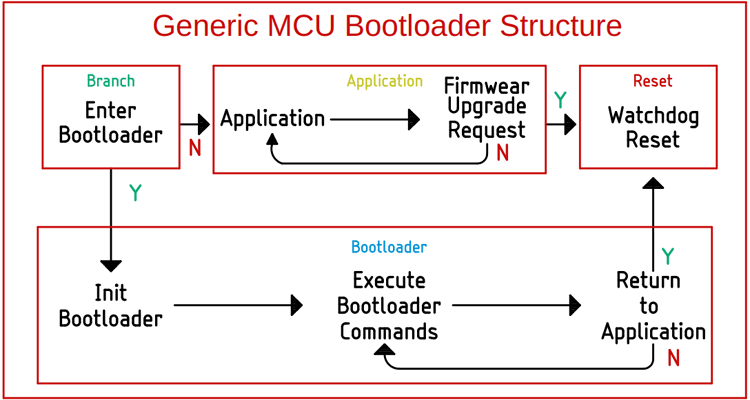
\includegraphics[scale=.33]{examples/Bootloader-System.png}}
\caption{Una struttura generica dell'algoritmo di Bootloader.}
\label{fig}
\end{figure}
\newline

Nella figura è evidenziato il flusso di struttura di codice che riguarda ad esempio l'aggiornamento di un sistema come il firmware per un microcontrollore.

Il sistema parte sempre da un Watchdog Reset che di fatto inizializza il sistema
elettronico e permette come prima operazione la scelta sul continuare ad utilizzare il vecchio codice, ovvero la scelta sì(Y) per "Return To Application" oppure il richiamo della funzione di bootloader in caso di No(N), una funzione che sovrascrive il codice eseguito in precedenza e di fatto esegue un aggiornamento del firmware stesso.

La struttura di codice è ovviamente periodica (termina con un reset e quindi permette una nuova iterazione delle stesse operazioni nel caso in cui l'aggiornamento non è quello voluto oppure si continua con il codice già presente.



\section{Il bootloader nell'MSP430}
Di seguito saranno elencate le principali modalità con cui i bootloader specifici per microcontrollori Texas Instrument vengono utilizzati e anche le funzionalità specifiche per questa tipologia di board.

La presenza sia di una FPGA che di un MCU, connessa al fatto della presenza di pin dedicati di JTAG, permettono diversi utilizzi che successivamente spiegheremo.
\subsection{Invocazione Hardware del Bootloader}

L’invocazione del bootloader in presenza di un pin di jtag condiviso nel MSP430 avviene applicando una determinata sequenza al determinato pin di JTAG (RST/NMI e TEST) presente sulla scheda.
L’imposizione di una determinata sequenza su questi due pin determina l’utilizzo del reset vector (localizzato nella locazione di memoria FFFEh del microcontrollore) nel caso in cui il pin TEST venga mantenuto a livello logico basso oppure l’inizio della sequenza di Bootloader nel caso in cui venga alzato per ben due volte secondo lo schema temporale che ora esaminiamo:

\begin{figure}[htbp]
\centerline{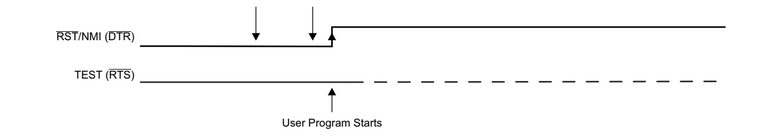
\includegraphics[scale=.7]{examples/resetSequence.PNG}}
\caption{la sequenza standard di RESET}
\label{fig}
\end{figure}

\begin{figure}[htbp]
\centerline{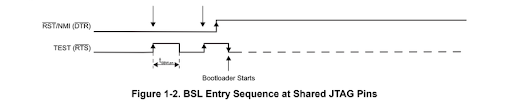
\includegraphics[scale=1.15]{examples/BSLEntrySequence.png}}
\caption{la sequenza standard di RESET utilizzando i pin condivisi di JTAG}
\label{fig}
\end{figure}


Ci sono inoltre dei fattori che prevengono l’invocazione del Bootloader (che non garantiscono il salto al BSL RESET vector) che bisogna garantire:
\begin{itemize}
\item Ci sono meno di \textbf{due fronti di salita} nel pin TEST mentre il pin RST/NMI rimane basso.
\item Il pin TEST non si mantiene al \textbf{livello logico alto} (come nella seconda figura precedente) quando il pin RST/NMI esegue il fronte di salita (dal livello logico basso ad alto).
\item \textbf{JTAG} ha il controllo delle risorse del microcontrollore MSP430.
\item L’alimentazione \textbf{$V_{CC}$} scende sotto un livello di soglia e un power-on reset (POR) viene eseguito.
\item Il pin \textbf{RST/NMI} viene configurato per la funzionalità NMI ( viene settato il bit di NMI).
 Se i pin TCK e TMS rimangono senza un riferimento a massa, il dispositivo potrebbe involontariamente entra in modalità JTAG. Ricordiamoci dunque di applicare dunque una terminazione esterna per questi due pin. ( Un resistore di pull-up con
resistenza pari a 47-k\ohm e una capacità di pull down pari ad un 1-nF sia sui pin di TCK che TMS.
\end{itemize}

\subsection{MSP430 con pin di JTAG dedicato}

L’invocazione del bootloader in presenza di pin di jtag dedicato utilizza i seguenti pin per lanciare il bootloader: RST/NMI e TCK.
Il programma di Bootloader viene utilizzato ogni volta che il pin di TCK vede per almeno due fronti di discesa il pin RTS/NMI alto.
Vediamo la figura:

\begin{figure}[htbp]
\centerline{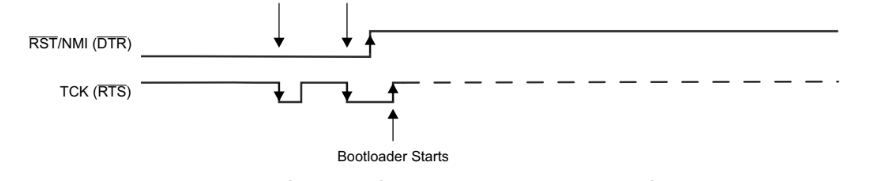
\includegraphics[scale=0.47]{examples/JTAGPin.png}}
\caption{la sequenza standard di START nel caso di pin dedicato di JTAG}
\label{fig}
\end{figure}

Anche in questo ci sono dei fattori che prevengono l’attivazione del bootloader:
\begin{itemize}
\item Il pin di \textbf{RST/NMI rimane basso} per un numero di fronti di discesa minore di due.
\item \textbf{TCK è alto} e \textbf{RST/NMI sale} dal valore logico basso a quello alto.
\item JTAG ha il controllo delle risorse del microcontrollore MSP430.
\item L’alimentazione $V_{CC}$ scende sotto un livello di soglia e un power-on reset (POR) viene eseguito.
\item Il pin \textbf{RST/NMI} viene configurato per la funzionalità NMI ( viene settato il bit di NMI).
\end{itemize}


\subsection{Dispositivi con un pin USB}

Nel caso di dispositivi con un pin USB ci sono semplicemente questi fattori che prevengono l’attivazione del bootloader:
\begin{itemize}
\item Il device è alimentato dall’USB e il \textbf{reset vector} non è scritto.
\item Il device viene alimentato con il pin PUR legato al \textbf{$V_{USB}$}.

\end{itemize}

\section{Invocazione Software del Bootloader}

Il Bootloader può essere invocato anche dal software (così avviene nel nostro caso).
Questo avviene all’interno da una parte di codice eseguita e di fatto setta il program counter all’indirizzo in memoria dove l’algoritmo di Bootloader è scritto. La locazione standard del bootloader è definita nei documentazione e nel nostro caso è localizzata nella locazione di memoria pari a 0x1000.

Il codice che permette il salto è il seguente:

\newline

\begin{lstlisting}[language=C]
__disable_interrupt();              // disable interrupts
((void ( * )())0x1000)();           // jump to BSL
\end{lstlisting}

\newline

Quando il bootloader viene eseguito lo stack viene resettato e la RAM viene pulita. 
Il bootloader non disabilita gli interrupt e di conseguenza è necessario disattivarli manualmente e riattivarli rispettivamente quando viene invocato l’algoritmo di bootloader e quando si ritorna al codice eseguito normalmente.

Le parole inviate tramite Bootloader vengono processate immediatamente dopo averle ricevute e le scritture di conseguenza avvengono sequenzialmente (non vi è un buffer dedicato interno al Bootloader).

Il periodo di scrittura è di conseguenza determinato dal baud rate e dal tipo di protocollo deciso per la comunicazione dei dati.

L’informazione comunicata al Bootloader viene codificata secondo il protocollo standard seriale (SSP).

Di seguito verranno presentati le principali caratteristiche per tutti protocolli di comunicazione utilizzati:

\subsection{Parametri Software per il Bootloader}

Il protocollo UART nel caso del Bootloader è definito con i seguenti parametri:

\begin{itemize}
\item Baud rate fisso a 9600 baud in half-duplex mode.
\item  Un singolo bit di Start, 8 bit di data LSB come primo bit), un bit di parità, 1 bit di stop.
\item Handshake eseguito tramite un carattere singolo di acknowledge.
\item Un ritardo minimo compreso nell’invio di un nuovo carattere definito nell’MSP430 pari a 1.2 msec
\end{itemize}

\subsection{Parametri per il protocollo USB}
Il protocollo USB nel caso del Bootloader è definito con i seguenti parametri:

\begin{itemize}
\item HID protocol con un singolo input endpoint ed un singolo output endpoint. Ogni endpoint ha una lunghezza di buffer pari a 64 bytes.
\item  VID: 0x2047
\item  PID: 0x0200
\end{itemize}


\subsubsection{Sequenza di sincronizzazione con protocollo USB}

Prima di mandare qualsiasi comando verso il microcontrollore riguardante il protocollo di Bootloader, è necessario inviare una carattere che permette la sincronizzazione (SYNC) pari a 0h80.

L’invio di questo carattere permette al Bootloader di calcolare tutti i parametri interni necessari al funzionamento del Bootloader.

Quando il carattere di SYNC viene ricevuto, in risposta si ha un altro byte di acknowledge pari a 0h90 inviato indietro dal Bootloader.
\vspace{0.5cm}
Elenco dei comandi di Bootloader non protetti da password:
\begin{itemize}
\item Receive password.
\item Mass erase (erase dell’intera flash memory).
\item Transmit BSL version .
\item Change baud rate  (per le versioni V1.60 or V1.61 or V2.0x ).
\end{itemize}
\vspace{0.5cm}
Elenco dei comandi di Bootloader protetti da password:

\begin{itemize}
\item Receive data block to program flash memory, RAM, or peripherals.
\item Transmit data block.
\item Erase segment.
\item Erase check (present in V1.60 or superiori).
\item Set Memory Offset (present in V2.12 or superiori).
\item Load program counter and start user program.
\item Change baud rate ( per le versioni inferiori di V1.60 e superiori a V2.10).
\end{itemize}

\section{Utilizzo del Bootloader per problemi di corruzioni della memoria}

Nel nostro caso il codice eseguito infatti è collocato nella memoria FLASH/RAM del dispositivo, ovvero una memoria più veloce della memoria flash ma facilmente corruttibile da agenti esterni come le radiazioni che durante la missione il satellite subisce.\newline

Queste radiazioni generano statisticamente delle inversioni di bit di alcune locazioni della memoria del dispositivo.

la procedura di Bootloader di riprogrammazione in questo caso della memoria FLASH/RAM è dunque necessaria per il mantenimento dell'integrità del codice eseguito, ovvero uno dei requisiti fondamentali per la "reliability" (affidabilità) del microcontrollore e conseguentemente per il corretto funzionamento dell'intero sistema.\newline

L'integrità di un codice viene valutata attraverso il confronto tra i valori di ridondanza calcolati sul codice correntemente eseguito e i valori di ridondanza preventivamente calcolati e collocati in una locazione precisa di memoria Flash.


Tale ridondanza viene calcolata tramite l'algoritmo CRC-16 ("Cyclic redundancy check"), ovvero un algoritmo che a partire da un flusso indefinito di bit definisce un risultato di lunghezza fissa (nel nostro caso 16 bit).\newline

La corruzione di alcuni bit, ovvero l'inversione 0-1 o 1-0 porta necessariamente ad un risultato diverso dell'algoritmo CRC-16.

Questi bit sono salvati in una zona dedicata di memoria ogni volta che si ha una fase di scrittura del codice firmware all’interno del microcontrollore e di conseguenza mantengono informazione relativa al codice attualmente eseguito.\newline

Conseguentemente, il confronto a posteriori della ridondanza valutata sul codice eseguito con i valori salvati permette la rivelazione di un’eventuale corruzione del codice.

Nel caso in cui venga dunque rilevata una differenza tra i due diversi valori di protezione un nuovo codice viene caricato. Ciò permette il normale e giusto funzionamento del codice eseguito poiché diverse copie contenenti lo stesso codice vengono caricate nel firmware se necessario.

Il codice che viene caricato deve essere comunque a sua volta non corrotto. Di conseguenza, prima di caricare il nuovo codice, il bootloader si premura di valutare l'integrità del nuovo codice.

Nel nostro caso le copie del codice originale sono molteplici e tutte note al bootloader (tramite la definizione dell'indirizzo iniziale in cui i codici di backup vengono collocati e della loro lunghezza).

Il bootloader di conseguenza si premura, nel caso di corruzione del codice corrente, di valutare sequenzialmente l'integrità di ogni possibile copia del codice originale e di caricare la prima versione integra disponibile.

Tutte le copie non sono precisamente uguali e di lunghezza più corta possibile, in quanto maggiore è la dimensione del codice, maggiore è la probabilità che almeno una delle locazioni di memoria di tale codice venga corrotto durante la missione.



\section{Creazione di una sezione di bootloader all'interno della memoria firmware in un microcontrollore}

La prima azione da compiere per inserire le versioni alternative di codice da caricare nel caso di una corruzione è quella di definire lo spazio di memoria flash in cui verranno poi collocati i codici di riserva.

Il bootloader utilizza  infatti una coppia di puntatori (rispettivamente in memoria flash e in memoria ram) e si occupa di leggere e sovrascrivere locazione per locazione l'intero codice,
partendo dall'indirizzo iniziale di entrambi i settori ( rispettivamente codice corrente e codice di riserva) e smarcando il puntatore di una singola locazione di memoria per un numero di volte pari alla lunghezza del nuovo codice.\newline

Tali valori vengono forniti al bootloader tramite delle apposite costanti in bootloader.h:

\begin{figure}[htbp]
\centerline{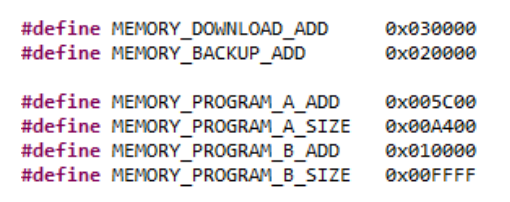
\includegraphics[scale=.7]{examples/BackupSection.PNG}}
\caption{La sezione in codice C riguardante la zona di memoria occupata nel microcontrollore dai codici di backup.}
\label{fig}
\end{figure}
\newpage
Per conoscere poi la lunghezza di tali versioni di backup bisogna consultare il linker script dedicato al progetto, ovvero un file in cui vengono definite tutte le sezioni di memoria del dispositivo e le loro funzioni:

\begin{figure}[htbp]
\centerline{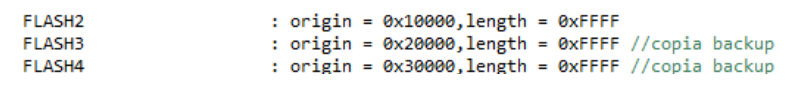
\includegraphics[scale=.67]{examples/PuntatoriDiStartBootloader.PNG}}
\caption{La sezione in codice C riguardante la definizione dei puntatori da cui iniziare a leggere i codici di backup.}
\label{fig}
\end{figure}

Il prossimo passo da compiere è quello di estrapolare il codice di backup che poi dovrà essere caricato all'interno del microcontrollore. \\
Code Composite Studio fornisce infatti una versione di codice eseguibile soltanto in formato ".txt" come la seguente (figura 3.7):
\begin{figure}[htbp]
\centerline{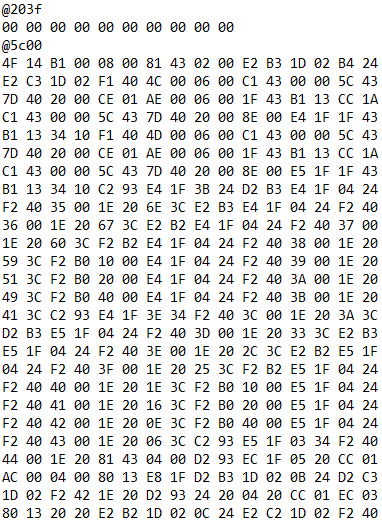
\includegraphics[scale=.67]{examples/TxtCodeBootloader.PNG}}
\caption{Esempio di codice sorgente in formato ".txt"}
\label{fig}
\end{figure}

Come possiamo notare, il codice sorgente fornito nella cartella del progetto compilato è diviso nelle diverse sezioni, ognuna specificata dalla sigla "@xxxx", ovvero la locazione di partenza in cui verranno poi collocate nelle zone di codice e dati. 

Ricordiamo che queste diverse sezioni sono già state definite nel file di bootloader.

Questo tipo di file deve essere dunque convertito in file ".bin" che potrà essere caricato direttamente all'interno della memoria.
\vspace{0.5cm}
Per fare ciò abbiamo a disposizione un programma chiamato "Msp430 Firmware Converter" che permette dunque la conversione dal formato ".txt" al formato binario desiderato.

Inseriamo dunque il firmware all'interno del programma tramite l'apposita funzione di caricamento di file scegliendo accuratamente la "Magicword" adatta per il tipo di firmware utilizzato:

\begin{figure}[htbp]
\centerline{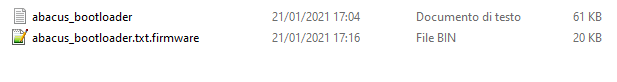
\includegraphics[scale=0.76]{examples/FileTiConverter.PNG}}
\caption{Quello che uscirà sarà dunque un file .bin come questo, ovvero un file binario disponibile all'interno della stessa cartella in cui è salvato il file .txt.}
\label{fig}
\end{figure}
\newline

Come ultimo passo andiamo a caricare i file binari all'interno della memoria in Code Composite Studio.
Questo può essere fatto utilizzando l'utility chiamata "Memory Browser", ovvero una applicazione che ci permette di leggere e scrivere direttamente le locazioni di memoria di tutto il microcontrollore durante la fase di debug.
\newpage
Prima di caricare il nuovo firmware assicuriamoci che la parte di memoria sia ancora non scritta: andiamo a digitare nel riquadro in alto l'indirizzo iniziale in cui dovrebbero essere i firmware di riserva.
\begin{figure}[htbp]
\centerline{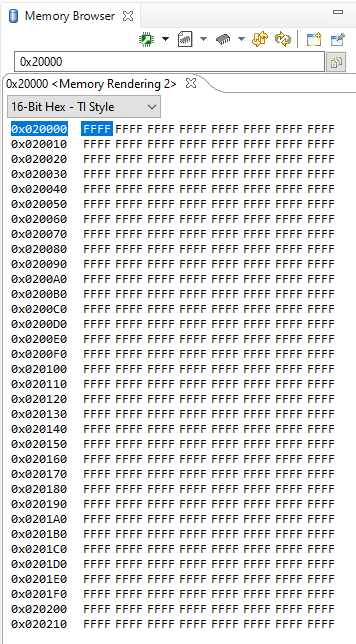
\includegraphics[scale=0.58]{examples/MemoryBrowserTi.PNG}}
\caption{Quello che uscirà sarà dunque un file .bin come questo, ovvero un file binario disponibile all'interno della stessa cartella in cui è salvato il file .txt.}
\label{fig}
\end{figure}
\newline


Come ci aspettavamo a partire da tali locazioni ogni singolo bit è pari ad 1 (ogni locazione è pari a 0xFFFF ). 

Questo significa per l'appunto che tale settore non è stato ancora scritto:
\clearpage

Andiamo dunque ad aggiungere il nuovo firmware tramite l'opzione in alto a sinistra "Load Memory".
Apparirà una finestra in cui bisogna specificare il percorso del firmware ed il suo formato (nel nostro caso Binary).

\begin{figure}[htbp]
\centerline{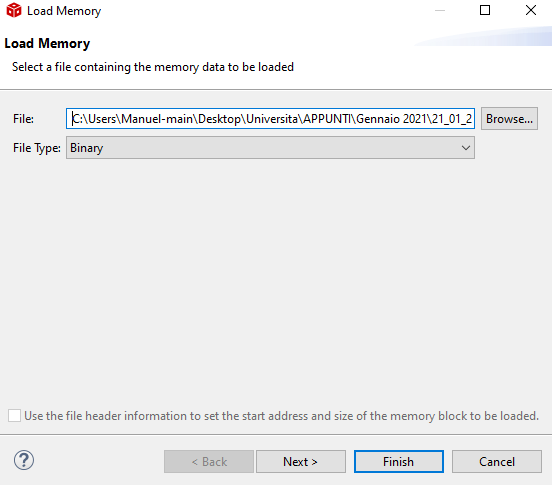
\includegraphics[scale=0.75]{examples/LoadMemory1.PNG}}
\caption{In questa sezione viene definito il file sorgente da caricare in memoria ed il tipo di file (nel nostro caso del codice sorgente ".bin".}
\label{fig}
\end{figure}
\newline

\clearpage
Clicchiamo "Next" per passare poi ad una nuova finestra in cui specifichiamo l'indirizzo  iniziale (in valore esadecimale) in cui collocare il file binario:


\begin{figure}[htbp]
\centerline{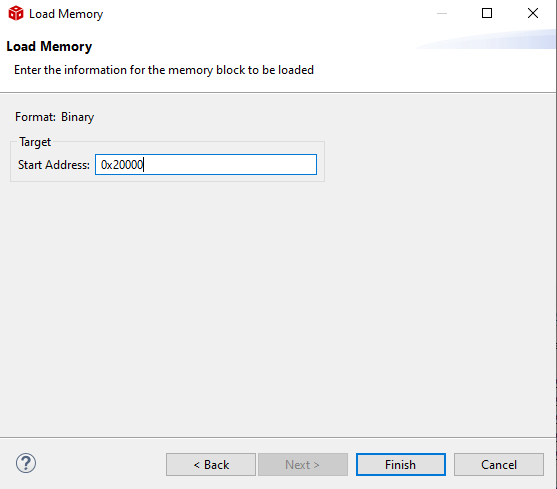
\includegraphics[scale=0.75]{examples/LoadMemory2.PNG}}
\caption{In questa sezione viene definito il target, ovvero la locazione assoluta in cui il backup verrà scritto.}
\label{fig}
\end{figure}
\newline


Una volta inserito premiamo "Finish" per caricare il nuovo firmware.
\clearpage
Valutiamo dunque che il nuovo firmware sia correttamente scritto nella parte di memoria scelta tramite Memory Browser.


\begin{figure}[htbp]
\centerline{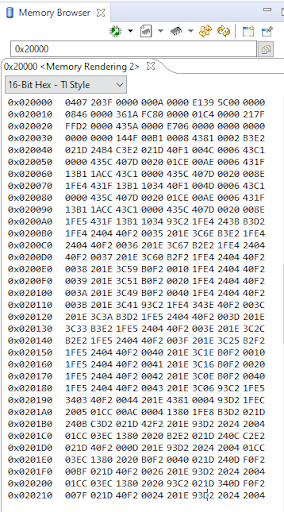
\includegraphics[scale=0.75]{examples/LoadedMemory.png}}
\caption{Parte di memoria in cui è collocato il primo codice di backup, collocato a partire dalla locazione desiderata (0x20000).}
\label{fig}
\end{figure}
\newline

Il firmware contenente il codice sorgente è stato correttamente caricato. 

A riprova di ciò, come si può notare nella figura 3.11, possiamo notare la "Magic Word" 0x07 decisa in fase di generazione del file binario e presente ora nella prima locazione di memoria al primo byte. ( "0x0407" , in cui "0x07" il logica "Little Endian" ci fornisce il prima byte sito nella locazione 0x20000 ).





\clearpage


\section{Struttura del codice di bootloader}

Andiamo ora a provare l'effettivo funzionamento del bootloader corrompendo manualmente durante la fase di debug determinati bit in memoria, in modo da innescare la procedura di bootloader.

Assicuriamoci di entrare nella parte di codice eseguito ciclicamente (la parte while(1) ) e blocchiamo il debugger.
\\\\
La procedura di controllo di integrità del firmware viene infatti invocata periodicamente in nella sezione che controlla l'integrità del codice in esecuzione.

Se vi sono quindi delle corruzioni all'interno del firmware corrente, il sistema si riavvierà tramite un reset generato modificando il valore di "watchdog timer" e portandolo a zero, causando dunque l'evento immediatamente.

Questo particolare timer non permette al microcontrollore di non rimanere in stallo (anche chiamato "deadlock"), ovvero controlla che sistematicamente delle nuove istruzioni vengano eseguite dal microcontrollore.

Ad ogni istruzioni eseguita il timer si resetta. Se invece supera la soglia significa che il sistema è bloccato.
\newline
Questa è la funzione che si occupa di verificare l’integrità del codice.
\footnote{Nota Bene: il valore 0xDEAD è un valore esadecimale totalmente casuale (diverso da 0) che permette al WatchDog Timer di scattare e di permettere un riavvio del codice a partire dalla sezione di start.}
\begin{lstlisting}[language=C]
    if(memory_mcu_checkProgramIntegrity(0) == -1 )
    {
        WDTCTL = 0xDEAD;
    }
\end{lstlisting}

Quello che facciamo nel caso di un riscontro di una corruzione è proprio forzare tale timer, scrivendo nel registro un valore superiore alla soglia, innescando il reset subito dopo.

Eseguito dunque il reset, la prima azione che il firmware compie sarà quella di verificare la corruzione del codice e dunque iniziare con il caricamento di un nuovo firmware integro.

Nelle prossime sezioni saranno valutati i possibili test case e verrà valutato il comportamento del microcontrollore.

\newpage
\section{Test dell'algoritmo di bootloader}
In questa sezione andremo ad esaminare tutti i test cases in cui il firmware presente sul microcontrollore utilizzerà l'algoritmo di bootloader, ovvero il codice eseguito in fase start-up e che permette di recuperare una copia di backup di codice presente in memoria FLASH utilizzabile come codice di rincalzo nel caso in cui il codice eseguito sia corrotto.

Questo meccanismo ci permette di eseguire una versione di codice integra e quindi indirettamente permette di rilevare e/o correggere corruzioni nel codice correntemente eseguito nel caso in cui codice eseguito e di backup coincidano.

Ogni test del funzionamento dell'algoritmo partirà da una situazione iniziale di codice operativo, ovvero oltre la fase di inizializzazione del microcontrollore, in modo da garantire una situazione reale e di intercettare quindi il comportamento del sistema nel caso in cui radiazioni esterne o interne siano presenti nel codice eseguito.

La modalità di studio del comportamento del codice in cui ci porremo sarà quella di debug, ovvero la modalità che permetterà di esaminare in tempo reale il contenuto delle singole locazioni di memoria .
Questa modalità ci permette anche di inserire delle corruzioni in singole locazioni sia di memoria RAM che di Flash, così da simulare delle corruzioni puntuali del memoria dell'MCU.

Tutte le verifiche e le corruzioni avverranno tramite il "Memory Browser" contenuto in CCS.

L'obiettivo finale di ogni test sarà quello di valutare la correttezza del codice eseguito, ponendoci da oracolo e valutando tramite l'osservazione diretta del controllo di integrità eseguito dall'algoritmo di controllo CRC-16 l'effettiva correzione delle corruzioni.\newline\newline
I requisiti che il sistema dovrà garantire durante l'esecuzione del codice saranno:
\begin{itemize}
    \item  Rivelazione e correzione di una corruzione del codice eseguito tramite una prima copia di backup.
    
    \item  Rivelazione e correzione di una corruzione del codice eseguito tramite una seconda copia di backup.
    
    \item  Rivelazione della corruzione del codice eseguito nel caso in cui nessuna delle copie di backup sia integra.
        
\end{itemize}


\subsection{Iniezioni di corruzioni all'interno del codice e avvio dell'algoritmo di correzione del codice}

Il primo test consiste dunque nella corruzione di una locazione casuale del firmware principale e nella valutazione della correzione del determinato registro tramite la procedura di bootloader.

Una volta caricato il firmware sul microcontrollore MSP430, facciamo partire il codice utilizzando lo strumento di debug fornito da CCS, in modo da valutare quali operazioni il microcontrollore esegue e anche per avere la possibilità di esaminare le variabile del codice eseguito. Questo controllo viene eseguito bloccando il codice che in teoria verrebbe eseguito sequenzialmente, fornendoci dunque una istantanea della situazione del microcontrollore in tempo reale.

La corruzione di una parte di codice può essere eseguita all'interno della finestra "Memory Browser" semplicemente cliccando sulla locazione di memoria da modificare e cambiando almeno uno dei valori contenuti nel valore esadecimale.
In questo modo il codice di controllo CRC utilizzato per controllare l'integrità del codice salvato potrà valutare un cambiamento all'interno dello spazio di memoria protetto e quindi innescare l'algoritmo di bootloader.

Una volta inserita la corruzione, clicchiamo "Enter" e continuiamo a far funzionare il firmware.
In questo caso il programma entra nel controllo dell'integrità e dopo aver rivelato la corruzione iniziando la procedura di reset.

\begin{figure}[htbp]
\centerline{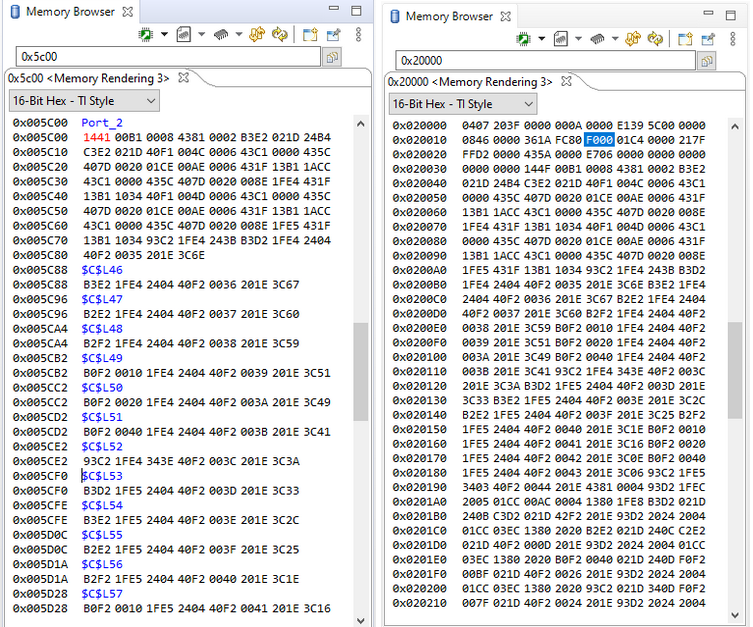
\includegraphics[scale=0.55]{examples/BootloaderTestCorruzioni2.PNG}}
\caption{Corruzione sia della sezione di RAM e del primo codice di backup.}
\label{fig}
\end{figure}
\newline

Il primo passo per far scattare la funzione di ripristino del codice eseguito tramite l'algoritmo di bootloader è quello di riconoscere la corruzione. Questa funzione di controllo dell'integrità del codice è eseguita dalla seguente parte di codice:

\begin{lstlisting}[language=C]
    int8_t memory_mcu_checkProgramIntegrity(uint8_t force)
{
    uint16_t crcBankA, crcBankB, crcBankACalc, crcBankBCalc;

    if(force == 0)
    {
        //Read values from config area MEMORY_PROGRAMINTEGRITY_ADD for banks A and B
        uint8_t buffer[5];
        abacus_flash_mcu_read_data(MCUMEMORY_PROGRAMINTEGRITY_ADD, buffer, 5);

        //First Magic word
        if(buffer[0] != MEMORY_MAGICWORD)
            force = 1;  //Force recalculation
        else
        {
            //Second CRC bank A
            char2uint(&buffer[1], &crcBankA);

            //Third CRC bank B
            char2uint(&buffer[3], &crcBankB);
        }
    }

    //Calculate CRC16 of Bank Aa
    crcBankACalc = abacus_flash_mcu_crc(MEMORY_PROGRAM_A_ADD, MEMORY_PROGRAM_A_SIZE);

    //Calculate CRC16 of Bank B
    crcBankBCalc = abacus_flash_mcu_crc(MEMORY_PROGRAM_B_ADD, MEMORY_PROGRAM_B_SIZE);

    //Save into memory the new CRC values
    if(force == 1)
    {
        //Delete the segment and save values:
        abacus_flash_mcu_erase(MCUMEMORY_PROGRAMINTEGRITY_ADD, 512);

        //Serialize the values:
        uint8_t buffer[5];
        buffer[0] = MEMORY_MAGICWORD;
        uint2char(&crcBankACalc, &buffer[1]);
        uint2char(&crcBankBCalc, &buffer[3]);

        //Save to MCU memory
        abacus_flash_mcu_write_data(MCUMEMORY_PROGRAMINTEGRITY_ADD, buffer, 5);

        //Exit indicating saved values
        return 1;
    }

    //Program integrity confirmed?
    if(crcBankACalc == crcBankA && crcBankBCalc == crcBankB)
        return 0;

    //Ups we have a memory corruption
    return -1;
}
\end{lstlisting}

La procedura di controllo dell'integrità della memoria viene richiamata periodicamente dal microcontrollore. Questa funzione si occupa di controllare in primo luogo la correttezza di un codice (la cosiddetta Magic Word presente in ogni copia) e successivamente si occupa di controllare tramite l'algoritmo CRC l'integrità dell'intero codice eseguito. Il test da esito negativo se i CRC valutati a priori e posteriori non coincidono.

Se tale test da esito negativo, il sistema viene riavviato tramite un software reset.


\begin{figure}[htbp]
\centerline{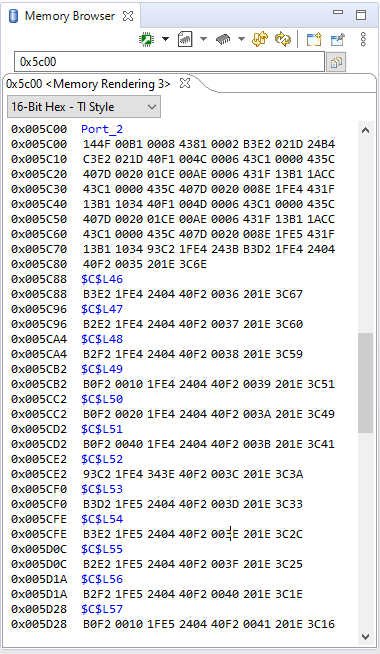
\includegraphics[scale=0.55]{examples/BootloaderTestCorruzioni3.PNG}}
\caption{Sezione di codice nuovamente corretta con la seconda versione di backup.}
\label{fig}
\end{figure}
\newline

Una volta reinizializzato il sistema il programma ora entra all'interno della funzione "bootloader start" e controlla nuovamente l'integrità del codice, riscontrando nuovamente un problema di consistenza dei dati. Tramite questa procedura il sistema attesta per due volte di seguito la corruzione di una locazione di codice e innesca quindi il vero e proprio algoritmo di bootloader (che viene solo avviato in fase di start del sistema). 

Il programma si occupa di ritrovare una copia integra di codice da poter utilizzare per sostituire quello vecchio corrotto.

Nel nostro caso il microcontrollore passa a valutare l'integrità della seconda copia, riscontrando in questo caso la correttezza della copia del codice e procedendo alla sovrascrittura del codice corrente. Il risultato è nuovamente la correzione del codice corrotto.

\begin{figure}[htbp]
\centerline{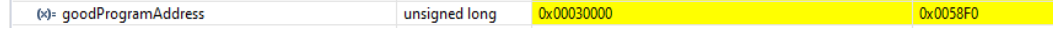
\includegraphics[scale=0.55]{examples/DebugBootloader.PNG}}
\caption{Valore che identifica la seconda versione del codice di backup, l'unica versione corretta.}
\label{fig}
\end{figure}
\newline

Una volta attestata la correttezza del codice di backup, l'algoritmo incomincia a sovrascrivere il codice precedente direttamente col nuovo codice integro. Ultimata questa procedura il codice dovrebbe ritornare dunque integro e nuovamente riutilizzabile.
\newline

\begin{lstlisting}[language=C]
    //check memory integrity
    int8_t result = memory_mcu_checkAlternativeProgramsIntegrity(0);
    if( result != -1 )
    {
        //Program is working good
        return 0;    
    }
    //Program is corrupted
    uint32_t goodProgramAddress;
    result = memory_mcu_checkAlternativeProgramsIntegrity(&goodProgramAddress);
    if( result == 0 )
    {
    //We have a possible candidate
    bootloaderTriggerRam(goodProgramAddress , 0 );
    
    return 0;
    }
    
    //No candidates for bootloader
    return -1;
    
\end{lstlisting}

\newline
Terminata tale fase, il sistema viene resettato in modo da poter controllare la correttezza del nuovo codice e successivamente ripartire con una nuova versione di codice da poter eseguire ciclicamente.

Completata tale procedura notiamo che il codice è nuovamente integro. Viene quindi mantenuta l'integrità del codice nonostante la corruzione del codice principale.

\begin{figure}[htbp]
\centerline{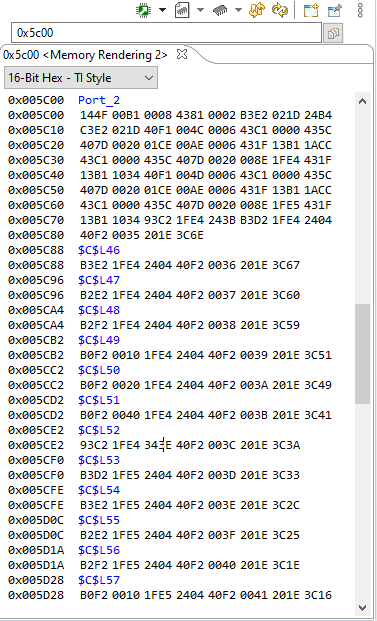
\includegraphics[scale=0.55]{examples/BootloaderTestCorruzioni1.PNG}}
\caption{Sezione di Memory Browser riferita sezione di codice originale.}
\label{fig}
\end{figure}


\subsection{Iniezioni di corruzioni di tutte le copie di backup di codice e valutazione del comportamento }

Infine, valutiamo con un ulteriore test una possibile fragilità di questo approccio. Come sappiamo il codice di bootloader è una sezione di codice che si occupa di correggere la restante parte del
codice in uso.

Di conseguenza, questa piccola parte deve rimanere integra per permettere al microcontrollore di valutare e correggere eventuali corruzioni.

\newline
Nel caso in cui delle radiazioni danneggiano una determinata locazione del codice di bootloader, è molto probabile che la procedura si blocchi e non funzioni portando dunque il microcontrollore
a due possibili comportamenti, ovvero:
\begin{itemize}
    \item Mantenimento della corruzione e continuazione dei task ordinari del sistema. Di conseguenza, una corruzione che non comporta un malfunzionamento del sistema.
    \item Danneggiamento della procedura di bootloader e loop infinita consistente nel tentativo di correzione del firmware e inevitabile reset causato dal watchdog timer per inattività del microcontrollore.
\end{itemize}


Per causare una corruzione del firmware di bootloader andiamo proprio a valutare la sua locazione all'interno del linker script, ovvero il file che fornisce il posizionamento di ogni sezione di codice presente in tutto il sistema.

Andiamo dunque a corrompere una delle locazioni di memoria del bootloader presente in RAM:

\begin{figure}[htbp]
\centerline{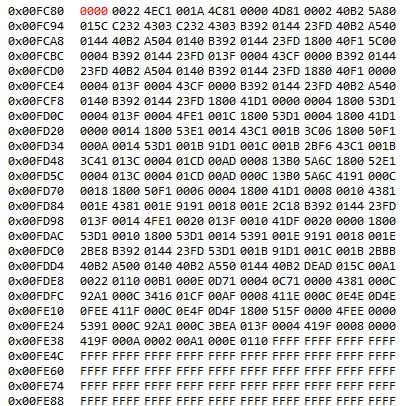
\includegraphics[scale=0.64]{examples/BootloaderCorruption.PNG}}
\caption{Corruzione della sezione di codice di Bootloader.}
\label{fig}
\end{figure}
\newline

Studiando con il debugger, figura 3.17, è possibile notare che l’errore nella sezione di bootloader viene riconosciuto ed il sistema viene riavviato:

\begin{figure}[htbp]
\centerline{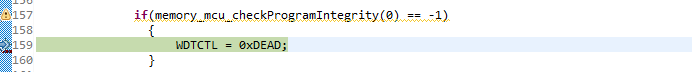
\includegraphics[scale=0.64]{examples/DebugCorruption.PNG}}
\caption{In fase di Debug, il codice riconosce l'errore all'interno del codice di bootloader attraverso un controllo tramite algoritmo CRC-16.}
\label{fig}
\end{figure}
\newline

Il problema sorge infatti dopo il riavvio, poiché il bootloader risulta corrotto e non correggibile. Nonostante ciò, il sistema continua nel funzionamento esponendoci però all’impossibilità di correggere eventuali corruzioni. 

Di conseguenza, il sistema risulta non più affidabile nel caso in cui il bootloader stesso venga corrotto.

\clearpage
\subsection{Codice sorgente dell'algoritmo di bootloader}

bootloader.h:

\begin{lstlisting}[language=c]
#ifndef BOOTLOADER_H_
#define BOOTLOADER_H_

#define BOOTLOADER_RAM_START_ADD 0x5900
#define BOOTLOADER_FLASH_START_ADD 0xFC80
#define BOOTLOADER_RAM_SIZE 0x0300
#define MCUFLASHBANKA 0x005c00
#define MCUFLASHBANKB 0x010000


#define MCUMEMORY_CONF_ADD         0x040000
#define MCUMEMORY_CONF_SIZE        0x001000
#define MCUMEMORY_PROGRAMINTEGRITY_ADD 0X041000

#define MEMORY_DOWNLOAD_ADD     0x030000
#define MEMORY_BACKUP_ADD       0x020000

#define MEMORY_PROGRAM_A_ADD    0x005C00
#define MEMORY_PROGRAM_A_SIZE   0x00A400
#define MEMORY_PROGRAM_B_ADD    0x010000
#define MEMORY_PROGRAM_B_SIZE   0x00FFFF

#define MEMORY_MAGICWORD        0x07


#include "memory/abacus_flash.h"
#include "memory/abacus_flash_mcu.h"
#include "abacus_utils.h"

int8_t bootloaderStart();

void bootloaderTriggerRam(uint32_t startAddress, uint8_t simulation);
void bootloaderFlash(uint32_t startAddress, uint8_t simulation);

// WDT for reset
#define WDT_MRST_LONG       (WDTCNTCL + WDTIS1 + WDTIS0)    // 500ms
#define WDT_MRST_EXTRALONG  (WDTCNTCL + WDTIS1)             // 8s
#define WDT_MRST_XXL        (WDTCNTCL + WDTIS0)             // 128s

#endif /* BOOTLOADER_H_ */
\end{lstlisting}
\clearpage
bootloader.c:

\begin{lstlisting}[language=c]

#include "bootloader.h"


#pragma CODE_SECTION(bootloaderStart,".text_bootloader")
#pragma CODE_SECTION(bootloaderTriggerRam,".text_bootloader")

/**
 * It checks the CRC of the banks A & B where program is stored and
 * saves the CRC on memory address bank A over the configuration address
 * If it fails it will load the memory from backup area (if CRC is also correct)
 * Force indicates if it has to ignore the CRC of the config area and recalculate
 * it, useful if new code has been added
 */
int8_t memory_mcu_checkProgramIntegrity(uint8_t force)
{
    uint16_t crcBankA, crcBankB, crcBankACalc, crcBankBCalc;

    if(force == 0)
    {
        //Read values from config area MEMORY_PROGRAMINTEGRITY_ADD for banks A and B
        uint8_t buffer[5];
        abacus_flash_mcu_read_data(MCUMEMORY_PROGRAMINTEGRITY_ADD, buffer, 5);

        //First Magic word
        if(buffer[0] != MEMORY_MAGICWORD)
            force = 1;  //Force recalculation
        else
        {
            //Second CRC bank A
            char2uint(&buffer[1], &crcBankA);

            //Third CRC bank B
            char2uint(&buffer[3], &crcBankB);
        }
    }

    //Calculate CRC16 of Bank Aa
    crcBankACalc = abacus_flash_mcu_crc(MEMORY_PROGRAM_A_ADD, MEMORY_PROGRAM_A_SIZE);

    //Calculate CRC16 of Bank B
    crcBankBCalc = abacus_flash_mcu_crc(MEMORY_PROGRAM_B_ADD, MEMORY_PROGRAM_B_SIZE);

    //Save into memory the new CRC values
    if(force == 1)
    {
        //Delete the segment and save values:
        abacus_flash_mcu_erase(MCUMEMORY_PROGRAMINTEGRITY_ADD, 512);

        //Serialize the values:
        uint8_t buffer[5];
        buffer[0] = MEMORY_MAGICWORD;
        uint2char(&crcBankACalc, &buffer[1]);
        uint2char(&crcBankBCalc, &buffer[3]);

        //Save to MCU memory
        abacus_flash_mcu_write_data(MCUMEMORY_PROGRAMINTEGRITY_ADD, buffer, 5);

        //Exit indicating saved values
        return 1;
    }

    //Program integrity confirmed?
    if(crcBankACalc == crcBankA && crcBankBCalc == crcBankB)
        return 0;

    //Ups we have a memory corruption
    return -1;
}


/**
 * It checks the integrity of programs downloaded into the MCU memory
 */
int8_t memory_mcu_checkAreaIntegrity(uint32_t startAddress)
{
    //Check how many chunks do we have to analize:
    uint8_t nchunks;

    //First read the magic word
    abacus_flash_mcu_read_data(startAddress, &nchunks, 1);
    if(nchunks != MEMORY_MAGICWORD)
        return -1;  //Nothing was there

    startAddress++;

    //Now read the number of chunks
    abacus_flash_mcu_read_data(startAddress, &nchunks, 1);

    startAddress++;

    //Sanity check
    if(nchunks == 0xFF)
        return -1;

    uint8_t i;

    uint32_t addressData = startAddress + (4 + 4 + 2) * nchunks;

    for(i = 0; i < nchunks; i++)
    {
        uint8_t buffer[10];
        uint32_t addressChunk, sizeChunk;
        uint16_t crcChunk, crcCalculated;
        abacus_flash_mcu_read_data(startAddress, buffer, 10);

        //address chunk 4 bytes
        char2ulong(&buffer[0], &addressChunk);

        //size chunk 4 bytes
        char2ulong(&buffer[4], &sizeChunk);

        //crc chunk 2 bytes
        char2uint(&buffer[8], &crcChunk);

        //calculate CRC of the selected chunk:
        crcCalculated = abacus_flash_mcu_crc(addressData, sizeChunk);

        if(crcCalculated != crcChunk)
            return -1;  //UPS incorrect area

        //Move to next chunk
        startAddress = startAddress + 10;
        addressData = addressData + sizeChunk;
    }

    return 0;
}

/**
 * It checks the integrity of Backup area and Download area (preference to backup)
 * if a valid program is found, it returns 0 and the start address
 */
int8_t memory_mcu_checkAlternativeProgramsIntegrity(uint32_t *goodStartAddress)
{
    //Read backup area:
    uint8_t result = memory_mcu_checkAreaIntegrity(MEMORY_BACKUP_ADD);

    if(result == 0)
    {
        *goodStartAddress = MEMORY_BACKUP_ADD;
        return 0;
    }

    result = memory_mcu_checkAreaIntegrity(MEMORY_DOWNLOAD_ADD);

    if(result == 0)
    {
        *goodStartAddress = MEMORY_DOWNLOAD_ADD;
        return 0;
    }

    return -1;
}

/**
 * It checks the integrity of the program (CRC16). If it fails, it will load the
 * backup program into flash memory. It uses abacus MCU memory functions, however
 * watch out, any other abacus functions do not work yet (no init called yet).
 */
int8_t bootloaderStart()
{
	//Go into a 8MHz version
	//Set DCO FLL reference = REFO
	UCSCTL3 |= SELREF_2;
	//Set ACLK = REFO
	UCSCTL4 |= SELA_2;
	//Disable the FLL control loop
	__bis_SR_register(SCG0);
	//Set lowest possible DCOx, MODx
	UCSCTL0 = 0x0000;

	//Select DCO range 8MHz operation
	UCSCTL1 = DCORSEL_5;
	//Set DCO multiplier:
	//(N + 1) * FLLRef = Fdco
	//245 * 32768 = 8MHz
	//Set FLL Div = fDCOCLK/2
	UCSCTL2 = FLLD_1 + 244;
	//Enable FLL Control loop
	__bic_SR_register(SCG0);
	//MCLK cycles for DCO to settle
	//32 * 32 * 8MHz / 32,768Hz = 250880 = MCLK
	__delay_cycles(250880);


	//Check memory integrity:
	int8_t result = memory_mcu_checkProgramIntegrity(0);
	if(result != -1)
	{
		//Program is just doing fine :)
		return 0;
	}

	//Program is corrupted! check for a backup or download programs:
	uint32_t goodProgramAddress;
	result = memory_mcu_checkAlternativeProgramsIntegrity(&goodProgramAddress);
	if(result == 0)
	{
		//we have a possible candidate!
		bootloaderTriggerRam(goodProgramAddress, 0);

		return 0;
	}

	return -1;
}

/**
 * It will check the integrity of the new program on the selected address
 * and if everything is correct it will load into RAM the code to flash
 * the program! it will finish with a PUC reboot
 */
void bootloaderTriggerRam(uint32_t startAddress, uint8_t simulation)
{
	//Sanity check, check again that there is a valid program on the selected
	//address
	int8_t result = memory_mcu_checkAreaIntegrity(startAddress);
	if(result == -1)
		return;

	//Copy function to memory RAM
	uint8_t *flash_start_ptr;
	uint8_t *ram_start_ptr;

	flash_start_ptr = (uint8_t *)BOOTLOADER_FLASH_START_ADD;
	ram_start_ptr = (uint8_t *)BOOTLOADER_RAM_START_ADD;

	// Copy flash function to RAM
	/*
	memcpy(ram_start_ptr,
			flash_start_ptr,
			BOOTLOADER_RAM_SIZE);*/
	uint16_t i;
	for(i = 0; i < BOOTLOADER_RAM_SIZE; i++)
	{
		*ram_start_ptr = *flash_start_ptr;
		ram_start_ptr++;
		flash_start_ptr++;
	}

	//Call function to memory RAM
	if(simulation == 0)
		bootloaderFlash(startAddress, simulation);
}


#pragma CODE_SECTION(bootloaderFlash,".text_bootloaderRam")
#pragma CODE_SECTION(bootloaderUChar2ULong,".text_bootloaderRam")

/**
 * External function on RAM to convert from byte to unsigned long
 */
void bootloaderUChar2ULong(uint8_t *input, uint32_t *output)
{
  typedef union
  {
    unsigned long longValue;
    uint8_t byteValue[4];
  }
  assocdata;
  assocdata conversion;
  int i;
  for(i = 0; i < 4; i++)
    conversion.byteValue[i] = input[i];

  *output = conversion.longValue;
}

/**
 * This is actually the function that is copied into the RAM! It takes 582 bytes!
 */
void bootloaderFlash(uint32_t startAddress, uint8_t simulation)
{
	// Stop watchdog timer
	WDTCTL = WDTPW | WDTHOLD;

	//Here we assume that all CRC were correct, so no more!

	//Disable all interrupts
	__bic_SR_register(GIE);
	__disable_interrupt();

	////////////////////////////////////////
	//Unlock Bank A and delete

	//Wait for memory to be ready
	while(FCTL3 & BUSY);

	// Clear LOCK & set LOCKA
	FCTL3 = FWKEY + LOCKA;
	//Set to erase
	FCTL1 = FWKEY + MERAS;

	//Wait for memory to be ready
	while(FCTL3 & BUSY);

	//Erase segment by segment:
	uint8_t *flashPointer;
	flashPointer = (uint8_t *) MCUFLASHBANKA;

	uint8_t i;

	while(FCTL3 & BUSY);

	//Dummy write, code is stopped until delete is completed
	*flashPointer = 0;

	/*for(i = 0; i < 82; i++)
	{
		//Wait for memory to be ready
		while(FCTL3 & BUSY);
		//Dummy write, code is stopped until delete is completed
		*flashPointer = 0;
		//Move to next segment
		flashPointer += 512;
	}*/

	//Wait for memory to be ready
	while(FCTL3 & BUSY);

	////////////////////////////////////////
	//Unlock Bank B and delete
	//Set to erase in BANK mode
	FCTL1 = FWKEY + MERAS;

	//Set to bank B
	while(FCTL3 & BUSY);
	flashPointer = (uint8_t *) MCUFLASHBANKB;

	//dummy write
	*flashPointer = 0;

	//Wait for memory to be ready
	while(FCTL3 & BUSY);



	//Unlock Bank A and B and set to write
	FCTL1 = FWKEY + WRT;
	//Wait for memory to be ready
	while(FCTL3 & BUSY);

	flashPointer = (uint8_t *)startAddress;
	//Jump magic code
	flashPointer++;
	//Read number chunks
	uint8_t nchunks = *flashPointer;
	flashPointer++;
	uint32_t addressInstall;
	uint32_t sizeInstall;

	volatile uint8_t *flashPointerInstall, *flashPointerRead;
	//uint32_t j;
	uint16_t sizeInstall16;

	flashPointerRead = (uint8_t *)startAddress;
	flashPointerRead += 2;
	for(i = 0; i < nchunks; i++)
	{
		flashPointerRead += 10 ;
	}

	for(i = 0; i < nchunks; i++)
	{
		bootloaderUChar2ULong(flashPointer, &addressInstall);
		flashPointer+=4;

		bootloaderUChar2ULong(flashPointer, &sizeInstall );
		sizeInstall16 = (uint16_t) sizeInstall;
		flashPointer+=6;	//Ignore CRC

		flashPointerInstall =  (uint8_t *)addressInstall;

		//I can't use the following because it is 32bit and uses a function on flash;
		//flashPointerRead = (uint8_t *)(startAddress + 1 + 1 + 10 * nchunks + dataCounter);

		uint16_t j = 0;

		for(j = 0; j < sizeInstall16; j++)
		{
			//Wait while busy
			while(FCTL3&BUSY);
			uint8_t byteNew = *flashPointerRead;
			*flashPointerInstall = byteNew;

			flashPointerInstall += 1;
			flashPointerRead += 1;
		}

		while(FCTL3 & BUSY);
	}

	//Relock memory flags:
	// Clear delete flags
	FCTL1 = FWKEY;
	FCTL3 = FWKEY + LOCKA + LOCK;

	//PUC Reboot writting incorrect value to WDT
	WDTCTL = 0xDEAD;
}
\end{lstlisting}



\chapter{Algoritmi di rivelazione e correzione dell'informazione}

La rilevazione e correzione dell'errore, in matematica, informatica, telecomunicazioni, e teoria dell'informazione, ha grande importanza pratica nel mantenimento dell'integrità dell'informazione nei sistemi con un canale rumoroso, o nei dispositivi per l'immagazzinamento dei dati caratterizzati da una scarsa affidabilità.
\newline
I meccanismi di base adottati a tale scopo sono l'introduzione sui dati generalmente da trasmettere o da memorizzare (come avviene nel nostro caso) di una certa ridondanza che permette di correggere (o quantomeno individuare) gli errori utilizzando un insieme limitato di valori ammissibili (tra tutte le combinazioni possibili) per la rappresentazione del dato e/o tramite l'analisi del contesto in cui si trovano i dati. 
\newline
Possiamo così riconoscere la presenza di errori in un dato quando ad esempio per effetto di uno o più errori questo modifica il suo valore in un valore non ammissibile o quando dall'analisi del contesto che lo circonda alcune regole di contesto sono violate. In alcuni casi l'entità dell'errore che colpisce il dato è limitata ed è possibile effettuare una ricostruzione corretta del dato (correzione dell'errore), mentre in altri casi permette solo il riconoscimento del deterioramento del dato e quindi rende possibile lo scarto dell'informazione (rivelazione dell'errore).
\newline
Nel nostro caso l'informazione soggetta a delle inversioni del valore logico di tensione dovuto alle corruzioni causate dalla radiazione spaziale é proprio il firmware del nostro microcontrollore. L'eventuale corruzione di alcune sezioni di memoria o di dati potrebbe generare comportamenti non voluti, malfunzionamenti e infine addirittura il fallimento della missione.
\newline
I codici che eseguono il compito di rivelare e eventualmente correggere l'informazione corrotta sono divisi in due tipologie: codici a blocchi e codici ad albero (o convoluzionali).
La prima tipologia di codici, i codici a blocchi (k,n)  trasforma una stringa binaria di lunghezza k-bit (definita come "dataword") in una nuova stringa binaria di lunghezza n (definita come "codeword"), senza sfruttare la memoria delle dataword precedenti.

Quando invece la corrispondenza tra dataword e codeword è caratterizzata da memoria, cioè gli n bit della codeword non dipendono solo dai k bit della dataword corrente ma anche dai bit di alcune dataword precedenti, il codice è detto ad albero.

La nostra trattazione riguarderà principalmente la prima tipologia di codice essendo i più adatti per un sistema di computer di bordo per un satellite, nel quale l'obiettivo principalmente è sia la gestione di diversi compiti e processi (quali il mantenimento del funzionamento generale della strumentazione e di raccoglimento ed elaborazione dei dati), sia un consumo limitato necessario per il mantenimento della batteria dell'intero satellite e quindi di conseguenza una potenza di calcolo relativamente limitata.

\newline
Nel nostro caso l'informazione soggetta a delle inversioni del valore logico di tensione dovuto alle corruzioni causate dalla radiazione spaziale é proprio il firmware del nostro microcontrollore.
L'eventuale corruzione di alcune sezioni di memoria o di dati potrebbe generare comportamenti non voluti, malfunzionamenti e infine addirittura il fallimento della missione.

\section{Definizione del canale binario simmetrico senza memoria e principali definizioni riguardanti la codifica di canale}

\begin{figure}[htbp]
\centerline{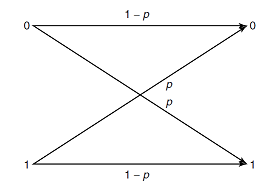
\includegraphics[scale=0.8]{examples/canale-binario.png}}
\caption{Modello di canale simmetrico (BSC) con probabilità di errore sul bit pari a p}
\label{fig}
\end{figure}
\newline
La figura 4.1 illustra il modello di un Canale Binario Simmetrico(BSC, Binary Symmetric Channel) mediante il grafo orientato. Un canale binario simmetrico è un semplice modello numerico senza memoria affetto da errori. In particolare, un BSC riceve in ingresso da una sorgente numerica singoli bit, con valore logico "0" o "1", e li consegna alla destinazione con uguale probabilità p di commettere un errore (ovvero di scambiare lo "0" con il valore "1" o viceversa per effetto di disturbi sul canale. 

La probabilità di errore è indipendente dagli errori commessi nella trasmissione di bit passati e futuri, per cui il canale è definito senza memoria.

Siano dati un blocco x costituito da n bit trasmessi $x_{n-1},....,x_1,x_0$ ed un blocco y costituito da n bit ricevuti $y_{n-1},....,y_1,y_0$, eventualmente soggetti a errori di trasmissione.

Per un BSC con probabilità di errore p la probabilità che all'interno del blocco di lunghezza n si verifichino m errori in corrispondenza di m prefissate posizioni è data da:
\begin{equation}
    P_{tot} = p^{m} (1-p)^{n-m}
\end{equation}

La probabilità che si abbiano m errori in posizioni qualunque sugli n bit trasmessi  è invece pari a:

\begin{equation}
    P_{tot2} = \binom{n}{m} p^{m} (1-p)^{n-m}
\end{equation}

Dove il coefficiente binomiale aggiunto è pari a:

\begin{equation}
    \binom{n}{m} = \frac{n!}{m! (n-m)!}  \hspace{2cm} con: n! = \prod_{j=1}^{n}j
\end{equation}


Le  prestazioni  di  un  codice  si  misurano  sulla  base  della
capacità di rilevazione e/o di correzione degli errori. Questi parametri sono definiti a seconda della tipologia di codifica di canale ed in particolare dipendono dall’efficienza (o rate di codice) $R_c=k/n$ (k → bit di messaggio, n → lunghezza
della parola di codice), che rappresenta il rapporto tra i bit di ridondanza utilizzati per ogni singolo blocco di informazione di lunghezza n.

Per  quantificare  matematicamente  il  concetto  della  separazione
tra  le  parole  di  codice,  definiamo  la  distanza  di  "Hamming"  e  la distanza minima del codice.

La distanza  di  "Hamming" d(X,Y)  tra  due  vettori  binari  X  e  Y  di
uguale  lunghezza  è  il  numero  di  bit  differenti  che  compaiono  nei due vettori in posizioni corrispondenti.

La distanza minima del codice $d_{min}$ è la minima distanza di
Hamming fra tutte le possibili coppie di parole di codice.


Se  si  è  verificato  un  numero  di  errori  minore  di  $d_{min}$,  la  parola
ricevuta non è una parola prevista dal codice e quindi è possibile
rilevare gli errori.

Se si è verificato un numero di errori maggiore o uguale a $d_{min}$, la
parola ricevuta potrebbe corrispondere ad una parola di codice. In
tal caso non sarebbe possibile rilevare gli errori.

La  regola  da  utilizzare  per  valutare  la  capacità  rilevativa  di  un
codice è la seguente:

\begin{equation}
    d_{min} \geq l + 1  
\end{equation}
Con un codice con capacità rilevativa pari a $l$ errori per parola.
\newline
Se  si  è  verificato  un  numero  di  errori  minore  di  $d_{min}/2$ , possiamo
correggere la parola ricevuta trasformandola nella parola di codice
più vicina.
\newline
Se  si  è  verificato  un  numero  di  errori  maggiore  o  uguale  a  $d_{min}/2$,
non possiamo correggere la parola ricevuta (la parola di codice ad
essa  più  vicina  potrebbe  non  essere  la  parola  che  era  stata
trasmessa).

La  regola  da  utilizzare  per  valutare  la  capacità  correttiva  di  un
codice è la seguente:

\begin{equation}
    d_{min} \geq 2t +1 
\end{equation}
Con un codice con capacità correttiva pari a $t$ errori per parola.



\section{Definizione dei principali tipi di algoritmi di correzione di errore}

Il principale impiego della codifica di canale è rendere la trasmissione il più affidabile possibile e quindi minimizzare la probabilità di errore. In accordo a come il sistema fa uso della potenzialità del codice, si può distinguere tra codici a rivelazione d'errore e codici a correzione d'errore. Questa distinzione non riguarda solo il codice impiegato ma soprattutto la strategia seguita dal sistema di co-decodifica.

I codici a rivelazione d'errore hanno lo scopo di verificare l'occorrenza di un errore nelle parole ricevute. Il decodificatore osserva la sequenza ricevuta all'uscita del demodulatore e rivela se sono avvenuti errori o meno. La rivelazione di eventuali errori è resa possibile dalla codifica di canale effettuata prima della trasmissione. 

Tra le tecniche di rivelazione degli errori più conosciute si menzionano:
\begin{itemize}
    \item Controllo di parità
    \item "Cyclic Redudancy Check" (CRC)
\end{itemize}

Entrambe sono basate su codici a blocchi.

La rivelazione d'errore è utilizzata per realizzare uno di due possibili schemi:
\begin{itemize}
    \item monitoraggio dell'errore (error monitoring): il decodificatore fornisce all'utente una indicazione continua sulla qualità della sequenza ricevuta, in modo che egli possa scartare la sequenza se l'affidabilità diviene troppo bassa;
    
    \item richiesta di ripetizione (ARQ, "Automatic Repeat reQuest"): si chiede al trasmettitore di ripetere la trasmissione fallite; deve essere disponibile un canale di ritorno (feedback) dal ricevitore al trasmettitore per segnalare l'occorrenza di errori rivelati dal decodificatore e richiedere ritrasmissioni di dati.
\end{itemize}


\newline
I codici a correzione di errore hanno invece lo scopo di rivelare l'occorrenza di errori nelle parole ricevute e di correggerli in modo da assicurare una corretta ricezione del messaggio trasmesso.

Il decodificatore tenta quindi di ripristinare la corretta sequenza trasmessa quando ci siano rivelati errori nella sequenza ricevuta. A parità di codice la "Forward Error Correction" (FEC) richiede algoritmi di decodifica più complessi rispetto a quelli di rivelazione d'errore con ARQ.


\subsection{Codice a controllo di ridondanza ciclico (CRC)}

Il CRC invece è una tecnica di codifica a blocco basata sul calcolo di somme di controllo ("checksum" in inglese) che in fase di codifica sono aggiunte (o appese) al blocco dei bit è informazione in base ai quali sono state calcolate. In fase di decodifica tali somme di controllo sono eseguite nuovamente sui bit ricevuti per riscontrare la congruenza tra i bit di informazione ed i bit di protezione ricevuti, così da rivelare la presenza di eventuali errori.

Ci sono diverse versioni del CRC in base alla lunghezza dei blocchi che vengono codificati. Ad esempio l'algoritmo CRC-16 utilizza blocchi di 16 bit ed ha una probabilità di errore di rivelazione d'errore pari a:

\begin{equation}
    P_{rivelazione fallita} = \sum_{k=0}^{\floor*{\frac{N}{2}}} P(k,N)
\end{equation}
    N: numero di bit in ogni gruppo

Dove il coefficiente polinomiale è definito come:
\begin{equation}
    P(k,N) =  \binom{N}{k} P_{b}^{k} (1-P_{b})^{N-k}
\end{equation}    
\subsection{Codice al controllo di parità: caratteristiche generali}

Il codice  a  controllo  di  parità  è un codice di controllo inserito al termine di un codice binario da trasmettere per rilevare eventuali errori di trasmissione.

Un  codice  a  controllo  di  parità  è  in  grado  di  rivelare  un
numero dispari di errori, questo perché il singolo bit di parità esegue l'operazione logica di "xor" ( $\oplus{}$ ) tra tutti i singoli bit, ritornando dunque un valore pari a 0 o 1 come bit di parità rispettivamente nel caso in cui il numero di 1 presenti all'interno della parole di codice si pari o dispari.

Il bit di parità, inserito normalmente successivamente alla dataword è così calcolato:

\begin{equation}
    b_{parity} =b_{0} \oplus{}  b_{1} \oplus{}  ...b_{n-1} \oplus{} b_{n} 
\end{equation}

Nella versione singolo bit di parità il codice permette soltanto di rivelare un numero dispari di errori mentre non permette di correggere nessun errore.
\newline
Nel prossimo paragrafo verrà esaminata una variante del codice di controllo di parità che permette addirittura la correzione di eventuali corruzioni. Questo perché l'obiettivo prefissato dall'algoritmo di scrubbing è quello di correggere subito eventuali corruzioni iniettate all'interno delle informazioni ed evitare in prima istanza una ritrasmissione dei dati presenti in memoria Flash (con un tempo di esecuzione maggiore) o addirittura un reset e dunque la perdita delle informazioni correnti.

\subsection{Codice di parità quadridimensionale: implementazione e prestazioni teoriche}

La versione utilizzata nella nostra implementazione è una evoluzione del codice di controllo di parità che condivide l’implementazione di base e la amplia al fine di correggere (oltre che rilevare eventuali errori) contenuti all’interno della struttura dati.

La struttura dati viene dunque disposta su matrice di bit (vedi figura 4.2) in cui ogni riga coincide con una dataword da proteggere.
La struttura matriciale permette dunque la protezione di strutture dati a lunghezza fissa (nel nostro caso sono dei byte, ovvero sequenze di caratteri a 8 bit) e la capacità correttiva è dunque definita a partire dal singolo blocco matriciale, generando quindi blocchi indipendenti.
L’implementazione classica calcolerebbe solo la “parità orizzontale” di ogni singola riga mentre nel nostro caso essendo una struttura bidimensionale è possibile ampliare il calcolo della parità sia per quanto riguarda la componente verticale che per quelle diagonali.
L’algoritmo quadridimensionale dunque si occupa di calcolare il bit di parità per queste quattro componenti:
\begin{itemize}
    \item parità orizzontale
    \item parità verticale
    \item parità diagonale destra
    \item parità diagonale sinistra
\end{itemize}

\begin{figure}[htbp]
\centerline{\includegraphics[scale=0.9]{examples/parita4D.PNG}}
\caption{Rappresentazione grafica dell'algoritmo di controllo di parità quadridimensionale}
\label{fig}
\end{figure}
\newline

Una volta ultimato il calcolo il calcolo ogni singolo bit di parità viene collocato in memoria in forma di ridondanza. 
Nell’esempio di 8 blocchi di parole (n parole) di lunghezza pari a 8 bit (m bit per parola), il numero di bit di parità è pari a 8+8+8+8=32 bit di ridondanza.

Se partiamo da una struttura matriciale (n x m), avremo un numero di bit pari a:
\begin{align}
L_{dataword} = (n * m) 
\end{align}
In generale, il numero di bit utilizzati è pari a :
\begin{align}
L_{codeword} = (n * m) + 2 * (m+n)
\end{align}

L'algoritmo è scalabile su blocchi di memoria di dimensione generalmente multipla di 8. In figura 4.3, è possibile valutare le prestazioni pratiche utilizzando diverse dimensioni.
\newline
L'algoritmo di parità quadridimensionale è stato confrontato con altri algoritmi di Forward Error Correction ed ha riscontrato il trade-off migliore tra capacità di correzione e bit overhead. I dati sono confrontabili in figura 4.4.

\begin{figure}[htbp]
\centerline{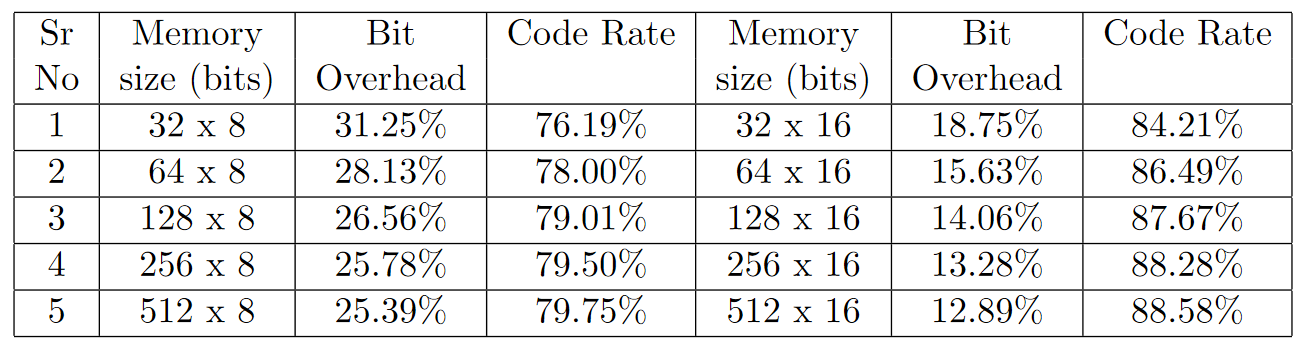
\includegraphics[scale=0.48]{examples/4dPerformance1.PNG}}
\caption{Prestazioni dell'algoritmo di parità 4d in base alla dimensione dei blocchi.}
\label{fig}
\end{figure}
\newline

\begin{figure}[htbp]
\centerline{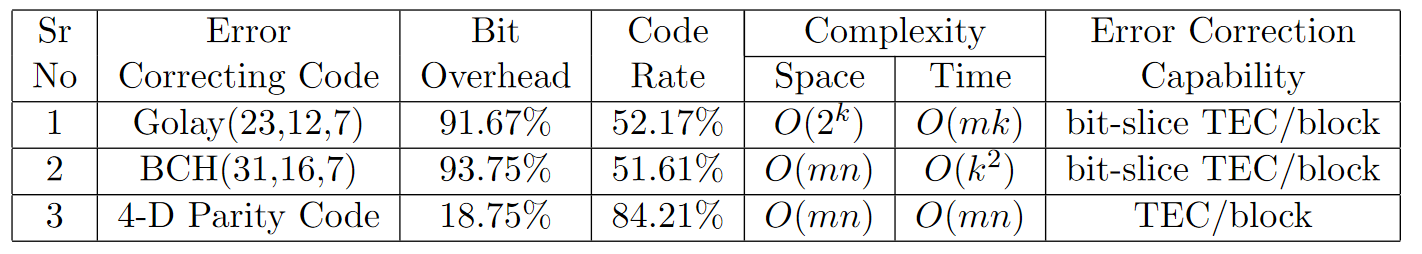
\includegraphics[scale=0.48]{examples/4dComparison.PNG}}
\caption{Confronto dell'algoritmo di parità 4d con altri algoritmi di codifica FEC.}
\label{fig}
\end{figure}
\newline

Di seguito confronteremo dunque i parametri fondamentali rispetto ad altri possibili codici da utilizzare.
Studiamo dunque le caratteristiche principali dell'algoritmo di parità quadridimensionale, valutando i pro e i contro dell'utilizzo di questo approccio nella Tabella 4.1:



\begin{table}
\begin{tabularx}{\linewidth}{>{\parskip1ex}X@{\kern4\tabcolsep}>{\parskip1ex}X}
\toprule
\hfil\bfseries Pro
&
\hfil\bfseries Contro
\\\cmidrule(r{3\tabcolsep}){1-1}\cmidrule(l{-\tabcolsep}){2-2}

%% PROS, seperated by empty line or \par

     Alto Code Rate (R), quindi basso bit overhead\par
    
     Tempo e spazio di calcolo lineare.\par
    
    Codifica e decodifica semplice.\par
    
    Applicabile a qualsiasi dimensione di memoria poichè utilizzabile su piccoli sezioni
    di memoria e facilmente scalabile.\par


&

%% CONS, seperated by empty line or \par
Capacità di rivelazione e correzione su singoli blocchi di memoria.\par

Necessità di processare l'intero blocco di memoria per correggere errori.\par


\\\bottomrule
\end{tabularx}
\caption{Pro e contro dell'algoritmo di parità 4d}
\end{table}

\clearpage

\section{Struttura del codice di scrubbing}


\subsection{Integrità dei dati del Registro di Stato del Satellite}

Il registro di stato del satellite è una struttura di dati che fornisce le informazioni necessarie per il monitoraggio e la gestione della missione spaziale. 

L’obiettivo del satellite è infatti quello di completare determinati task, tra cui degli esperimenti di natura chimica, i quali hanno una propria durata temporale e delle determinate azioni da eseguire. 

Per far ciò, il microcontrollore fornisce la lista di task e gestisce l’ordine temporale dell’esecuzione di quest’ultimi.
Il registro di stato del satellite fornisce la lista di informazioni al microcontrollore con cui può gestire l’andamento dei task.

Il mantenimento dell’integrità delle informazioni del registro di stato anche in caso di reset ( dovuti a vari motivi come ad guasti di parte del sistema, corruzione di parte della memoria o blocco delle azioni del satellite) permette al microcontrollore di risalire alle ultime informazioni salvate e di conseguenza fornisce la possibilità di una ripartenza non dal punto di inizio della missione (quindi dalla vera e propria inizializzazione del sistema), ma piuttosto dall'ultimo punto di backup salvato. 

In assenza di questo meccanismo di backup periodico il microcontrollore sarebbe costretto a resettare tutto il sistema e sarebbe necessariamente obbligato alla ripartenza del sistema dallo stato iniziale generando così un andamento dei task non coincidente con lo scheduling originariamente determinato in partenza.



\subsection{Gestione del registro di stato del satellite dopo un reset
}
Descriviamo ora quali azioni il microcontrollore esegue nel caso di un reset del sistema.
La strategia di base per mantenere integro il registro è la tecnica chiamata "Information redundancy", ovvero l’azione di generare periodicamente copie di parti di registro di stato necessarie per la ripartenza in zona di memoria distanti dall’originale. 
\newline
Tali copie vengono generalmente tenute da parte in assenza di malfunzionamenti. Se invece è riscontrato un problema nella memoria principale, il contenuto delle copie viene consultato, controllato nell'integrità a sua volta ed infine copiato al posto dei valori corrotti.

Questa strategia permette al microcontrollore di ripartire con una certa probabilità da una sezione dei task antecedente al reset e quindi non obbliga quest’ultimo a ripristinare all'interno della memoria i valori iniziali (come se fosse un primo avvio del sistema).
Descriviamo dunque le varie versioni del registro di stato presenti nel microcontrollore:
\begin{itemize}
    \item SatelliteStatus: la versione originale, si trova nella memoria SRAM ed è etichettata nel codice con la direttiva \#PRAGMA PERSISTENT, che obbliga il sistema ad inizializzarla soltanto durante il primo avvio con dei valori scelti per poi mantenerla con i valori già conosciuti anche nel caso di un riavvio (un software reset) semplicemente non inizializzando nuovamente i valori. 
    Soltanto nel caso di Power Reset la memoria SRAM, essendo una memoria volatile perde di fatto i valori correnti salvati e ritorna non inizializzata. In questo caso sarà necessaria in ogni caso una nuova inizializzazione o con i valori salvati nelle altre copie o con i valori di default.
    
    \item SatelliteStatusRamBackup: la versione di backup in memoria SRAM, ha anch’essa l’etichetta \#PRAGMA PERSISTENT e viene periodicamente sovrascritta durante la gestione di ogni task.Viene mantenuta continuamente integra e non soggetta a corruzioni da un algoritmo di scrubbing, ovvero un codice che tramite una ridondanza permette di evidenziare eventuali corruzioni e di correggerle (fino a 2 bit errati ogni blocco da 8 byte).
    In questo modo, è possibile mitigare il fenomeno della corruzione dei dati e limitare il disturbo generato dalle radiazioni cosmiche a cui il satellite è soggetto in orbita.
    Poiché l’algoritmo di scrubbing non garantisce sempre la correzione delle corruzioni, prima di eseguire il ripristino dei valori nella versione di backup, il sistema si assicura dell'assenza di errori in tutta la memoria. In questo modo il ripristino dei valori in SRAM viene effettuato soltanto nel caso in cui venga assicurata al coincidenza di parità di parità quadridimensionali a priori o posteriori. In caso contrario, si è scelto di scartare i valori in SRAM e di fare affidamento a quelli in memoria FLASH che successivamente descriverle.
    
    \item SatelliteStatusRomBackup: la versione di backup in memoria flash, la quale risulta una memoria non volatile e più protetta rispetto alle radiazioni. 
Il backup del registro di stato viene eseguita in questa memoria soltanto per quanto riguarda gli eventi critici, in quanto questa memoria risulta più lenta rispetta alla memoria SRAM specialmente nel caso di riscrittura dei dati, essendo scrivibile soltanto per pagine e non per singole locazioni.
Anche questa copia ha una parte di ridondanza valutata sempre tramite l’algoritmo CRC-16 e scritta sempre in ROM in una locazione vicina. Questa ridondanza è necessaria per valutare l’integrità di questa copia. Nel caso non venga verificata l’integrità, come misura di sicurezza si è deciso di caricare nel registro di stato i valori di inizializzazione.
\end{itemize}

Durante la fase di testing, abbiamo eseguito una valutazione del il tempo di esecuzione del codice (per quanto riguarda la fase di correzione del registro di stato del satellite) ed il valore trovato è stato di circa 2 msec per blocco di persistentRam (pari a 8 byte).


\begin{figure}[htbp]
\centerline{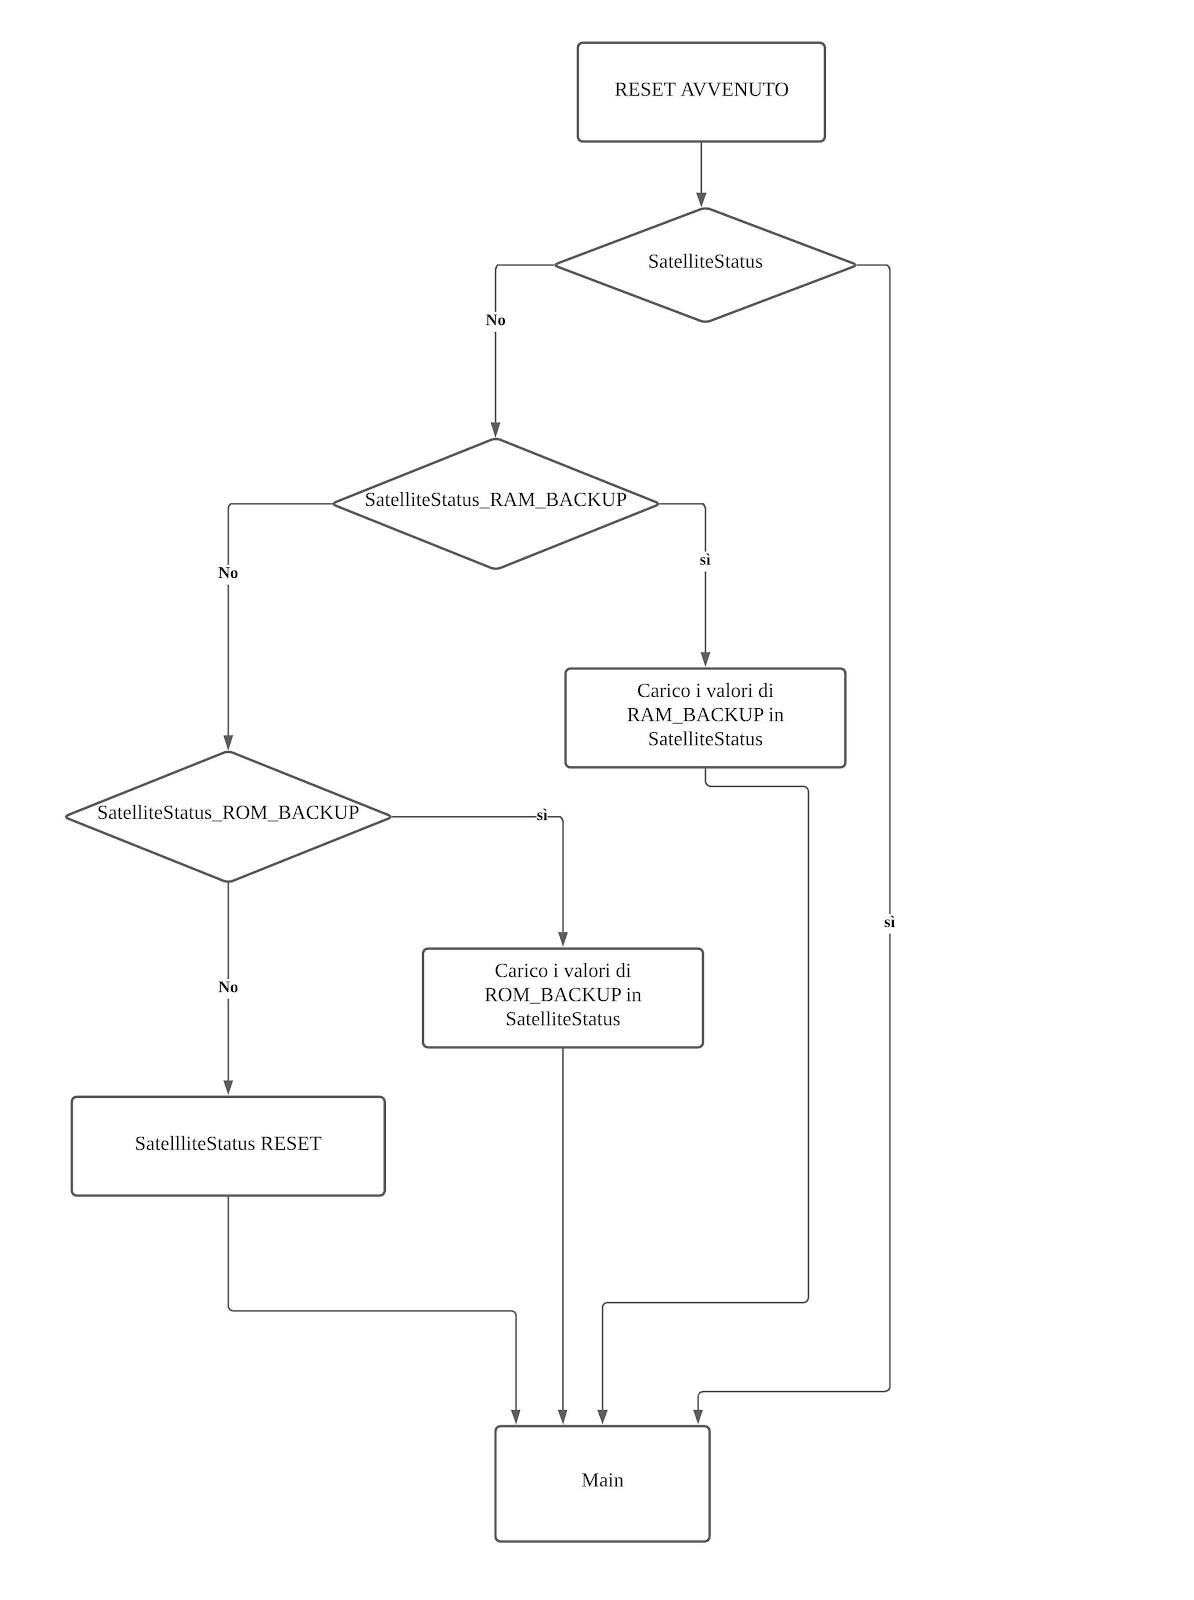
\includegraphics[scale=0.33]{examples/DiagrammaFlussoScrubbing.jpeg}}
\caption{Diagramma di flusso della parte dell'algoritmo di scrubbing (fase di inizializzazione del microcontrollore)}
\label{fig}
\end{figure}

\clearpage

\subsection{Codice sorgente dell'algoritmo di scrubbing}

Scrubbing.h:
\begin{lstlisting}[language=c][fontsize=\small]
#ifndef SCRUBBING_H_
#define SCRUBBING_H_
#include "abacus.h"
#include "satellite/configuration.h"
#include "PersistentRam/PersistentRam.h"


uint8_t scrubbingRoutine();


uint8_t periodicScrubPersistentRAM();


#endif /* SCRUBBING_H_ */
\end{lstlisting}
Scrubbing.c:
\begin{lstlisting}[language=c][fontsize=\small]
#include "PersistentRam/PersistentRam.h"
#include "BackupRom/BackupRom.h"
#include "satellite/satsystem_init.h"

#define ROM_BACKUP_AVAILABLE 0
uint8_t scrubbingRoutine()
{

    uint32_t i;
    uint8_t isPersistentRamUncorrupted = 0;
    for ( i=0; i<PERSISTENT_RAM_LENGTH/8; ++i) {
        if(scrub_recovery((uint8_t*)ramBackup_.persistentRam[8*i],i)!=0x0) {
            isPersistentRamUncorrupted = 0xff;
            break;
        }
    }
    if( isPersistentRamUncorrupted && ramBackup_.isPersistentRamWritten ) {
        restoreFromPersistentRam((uint8_t*)&ramBackup_.persistentRam[0],(uint8_t*)&satelliteStatus_,PERSISTENT_RAM_LENGTH);
    }
    else
    {

#if ROM_BACKUP_AVAILABLE
        if( isRomBackupPossible((uint32_t)ROM_BACKUP_STARTING_POINTER,(uint32_t)PERSISTENT_RAM_BYTE_SIZE) )
        {
            restoreDataFromRomBackup((uint32_t)MEMORY_TO_BACKUP_STARTING_POINTER, (uint32_t)ROM_BACKUP_STARTING_POINTER, (uint32_t)PERSISTENT_RAM_BYTE_SIZE);
        }
#endif

        backupInPersistentRam((uint8_t*)&ramBackup_.persistentRam[0], (uint8_t*)&satelliteStatus_, PERSISTENT_RAM_LENGTH);
    }

    return 0;
}


uint8_t periodicScrubPersistentRAM(){
    uint32_t r;
    for ( r = 0; r< PERSISTENT_RAM_LENGTH/8 ; ++r ) {
        scrub_recovery((uint8_t*)&ramBackup_.persistentRam[8*r],PERSISTENT_RAM_LENGTH/8);
    }
}

\end{lstlisting}
RomBackup.h:
\begin{lstlisting}[language=c][fontsize=\small]
#ifndef BACKUPROM_H_
#define BACKUPROM_H_

#include "../PersistentRam/PersistentRam.h"
#include "memory/abacus_flash.h"
#include "memory/abacus_flash_mcu.h"
#include "abacus_utils.h"
struct RomBackup
{
    uint8_t persistentRam[PERSISTENT_RAM_LENGTH];
    uint16_t crc16BackupData;
}romBackup;

#define ROM_BACKUP_STARTING_POINTER 0x28000
#define ROM_BACKUP_BLOCK_SIZE 512

extern struct RamBackup ramBackup_;

void setCrcInRomBackup();

int16_t getCrcInRomBackup();

uint8_t backupDataInRomBackup(uint32_t dataStartingAddress, uint32_t backupStartingPointer, uint32_t size);

uint8_t restoreDataFromRomBackup(uint32_t dataStartingAddress, uint32_t backupStartingPointer, uint32_t size);

uint8_t isRomBackupUncorructed(uint32_t dataStartingAddress, uint32_t size);

uint8_t isRomBackupPossible(uint32_t dataStartingAddress, uint32_t size);

#endif /* BACKUPROM_H_ */


\end{lstlisting}

RomBackup.c:
\begin{lstlisting}[language=c][fontsize=\small]
#include "BackupRom.h"
#include "abacus.h"
#include <math.h>
void setCrcInRomBackup()
{

}
int16_t getCrcInRomBackup()
{
    return romBackup.crc16BackupData;
}
uint8_t backupDataInRomBackup(uint32_t dataStartingAddress, uint32_t backupStartingPointer, uint32_t size)
{
    uint8_t result = 0x00;

    if(abacus_flash_mcu_erase(backupStartingPointer, size))
    {
        abacus_flash_write_data(AB_FLASH_MCU,(uint32_t)backupStartingPointer,(uint8_t*)dataStartingAddress,size);
        uint16_t* crcValue=&romBackup.crc16BackupData;
        calculate_crc16((uint16_t*)backupStartingPointer, size, crcValue, 1);

        result=0xff;


    }
    return result;
}

uint8_t restoreDataFromRomBackup(uint32_t dataStartingAddress, uint32_t backupStartingPointer, uint32_t size)
{
    uint8_t result = 0x00;
    uint16_t crcValue=0xffff;
    calculate_crc16((uint16_t*)backupStartingPointer, size, (uint16_t*)&crcValue, 1);

    if(crcValue==romBackup.crc16BackupData)
    {
        uint8_t* data = (uint8_t*)dataStartingAddress;
        abacus_flash_read_data(AB_FLASH_MCU, dataStartingAddress, data, PERSISTENT_RAM_LENGTH);


        result=0xff;
    }

    return result;
}

uint8_t isRomBackupUncorructed(uint32_t dataStartingAddress, uint32_t size)
{
    uint8_t result = 0x00;
    uint16_t crcValue=0xffff;
    calculate_crc16((uint16_t*)dataStartingAddress, size, (uint16_t*)&crcValue, 1);

    if(crcValue==romBackup.crc16BackupData)
    {
        result=0xff;
    }
    return result;
}

uint8_t isRomBackupPossible(uint32_t dataStartingAddress, uint32_t size)
{
    return ( (romBackup.crc16BackupData != 0x00) && isRomBackupUncorructed(dataStartingAddress,size) );
}

\end{lstlisting}

PersistentRam.h:
\begin{lstlisting}[language=c][fontsize=\small]
#ifndef PERSISTENTRAM_H_
#define PERSISTENTRAM_H_

#include "abacus.h"


#define SCRUBBING_PERSISTENT_RAM_LENGTH 80

void toggle_bit(int16_t Data[8],int16_t len,int16_t i,int16_t j);

int16_t Calc_HParity(int16_t Data[]);

int16_t Calc_VParity(int16_t Data[]);

int16_t Calc_DParity(int16_t Data[]);

int8_t scrubbing_bytes(int16_t Data[8],int8_t index);

int16_t find_position(int16_t a, int16_t *ptr);

void initialize(int16_t *pt, int16_t size);

int16_t count_errors(int16_t a);

void scrubbing_parity_generation(int16_t Data[8],int8_t stage,int8_t index );

void setScrubParity(uint8_t* index_pointer, uint8_t index_struct );

int8_t scrub_recovery(uint8_t* index_pointer, uint8_t index_struct );

void backupInPersistentRam (uint8_t* persistentStartingPointer,
                           uint8_t* memoryStartingPointer,
                           uint32_t length);
void restoreFromPersistentRam ( uint8_t* persistentStartingPointer,
                                uint8_t* memoryStartingPointer,
                                uint32_t length);

uint8_t cleanPersistentRam(uint16_t *byteElements, uint32_t size);

#define PERSISTENT_RAM_LENGTH 80
#pragma PERSISTENT(parity_)
struct parity
{
    int8_t h1[SCRUBBING_PERSISTENT_RAM_LENGTH/8];
    int8_t v1[SCRUBBING_PERSISTENT_RAM_LENGTH/8];
    int16_t d1[SCRUBBING_PERSISTENT_RAM_LENGTH/8];

    int8_t h2[SCRUBBING_PERSISTENT_RAM_LENGTH/8];
    int8_t v2[SCRUBBING_PERSISTENT_RAM_LENGTH/8];
    int16_t d2[SCRUBBING_PERSISTENT_RAM_LENGTH/8];
}parity_;
#pragma PERSISTENT (ramBackup_)
struct RamBackup
{
    uint8_t persistentRam[PERSISTENT_RAM_LENGTH];
    uint8_t isPersistentRamWritten;
}ramBackup_;


#endif


\end{lstlisting}

PersistentRam.c:
\begin{lstlisting}[language=c][fontsize=\small]
#include "PersistentRam.h"
#include <time.h>
#include <stdlib.h>
//struct RamBackup ramBackup_;

int16_t Calc_VParity(int16_t Data[])
{
    int16_t parity = 0;
    int16_t i;
    for(i=0; i<8; i++)
    {
        parity = parity ^ Data[i];
    }
    return parity;
}

int16_t Calc_HParity(int16_t Data[])
{
    int16_t parity = 0;
    int16_t temp;
    int16_t i,j, index;
    for(i=0; i<8; i++)
    {
        index = 0x80;
        temp = 0;
        for(j=0; j<8; j++)
        {
            if(Data[i] & index)
            {
                temp = temp ^ 0x0100;
            }
            index = index >> 1;
        }
        parity = parity ^ temp;
        parity = parity >> 1;
    }
    return parity;
}

int16_t Calc_DParity(int16_t Data[])
{
    int16_t parity = 0;
    int16_t dparity = 0;
    int16_t temp;
    int16_t i,j, index;
    for(i=0; i<8; i++)
    {
        index = 0x01;
        temp = 0;
        for(j=i; j>=0; j--)
        {
            if(Data[j] & index)
            {
                temp = temp ^ 0x0100;
            }
            index = index << 1;
        }
        parity = parity ^ temp;
        parity = parity >> 1;
    }

    for(i=1; i<=7; i++)
    {
        index = 0x80;
        temp = 0;
        for(j=i; j<=7; j++)
        {
            if(Data[j] & index)
            {
                temp = temp ^ 0x80;
            }
            index = index >> 1;
        }
        dparity = dparity ^ temp;
        dparity = dparity >> 1;
    }
    dparity = dparity << 8;
    dparity = dparity ^ parity;

    return dparity;
}

int8_t scrubbing_bytes(int16_t Data[8],int8_t index)
{
    int16_t h[8],v[8],d[16];
    int8_t dn, hn, vn;

    hn = count_errors(parity_.h2[index] ^ parity_.h1[index]);
    vn = count_errors(parity_.v2[index] ^ parity_.v1[index]);
    dn = count_errors(parity_.d2[index] ^ parity_.d1[index]);
    find_position(parity_.h2[index] ^ parity_.h1[index], h);
    find_position(parity_.v2[index] ^ parity_.v1[index], v);
    find_position(parity_.d2[index] ^ parity_.d1[index], d);

    if(hn==0 && vn==0 && dn==0)
    {
        return 0;
    }
    if((hn==1 && vn==1 && dn==1) && (d[0]==h[0]+v[0]))
    {
        toggle_bit(Data,8,h[0],v[0]);
    }
    if((hn==1 && vn==1 && dn==1) && (d[0]!=h[0]+v[0]))
    {
        if(d[0]<(h[0]+v[0]))
        {
            toggle_bit(Data,8,h[0],v[0]-1);
            toggle_bit(Data,8,h[0]-1,v[0]);
            toggle_bit(Data,8,h[0]-1,v[0]-1);
        }
        else
        {
            toggle_bit(Data,8,h[0],v[0]+1);
            toggle_bit(Data,8,h[0]+1,v[0]);
            toggle_bit(Data,8,h[0]+1,v[0]+1);
        }
    }
    if((hn==1 && vn==1 && dn==3) && (d[1]==h[0]+v[0]))
    {
    }
    if(hn==2 && vn==2 && dn==2)
    {
        if(d[0]==h[0]+v[0])
        {
            toggle_bit(Data,8,h[0],v[0]);
            toggle_bit(Data,8,h[1],v[1]);
        }
        else
        {
            toggle_bit(Data,8,h[1],v[0]);
            toggle_bit(Data,8,h[0],v[1]);
        }
    }
    if(hn==0 && vn==2 && dn==2)
    {
        toggle_bit(Data,8,(d[0]-v[0]),v[0]);
        toggle_bit(Data,8,(d[1]-v[1]),v[1]);
    }
    if(hn==2 && vn==0 && dn==2)
    {
        toggle_bit(Data,8,h[0],(d[0]-h[0]));
        toggle_bit(Data,8,h[0],(d[1]-h[1]));
    }
    if(hn==2 && vn==2 && dn==0)
    {
        toggle_bit(Data,8,h[0],v[1]);
        toggle_bit(Data,8,h[1],v[0]);
    }
    if(hn==1 && vn==3 && dn==3)
    {
        toggle_bit(Data,8,h[0],v[0]);
        toggle_bit(Data,8,h[0],v[1]);
        toggle_bit(Data,8,h[0],v[2]);
    }
    if(hn==3 && vn==1 && dn==3)
    {
        toggle_bit(Data,8,h[0],v[0]);
        toggle_bit(Data,8,h[1],v[0]);
        toggle_bit(Data,8,h[2],v[0]);
    }
    if(hn==3 && vn==3 && dn==1)
    {
        toggle_bit(Data,8,h[2],v[0]);
        toggle_bit(Data,8,h[1],v[1]);
        toggle_bit(Data,8,h[0],v[2]);
    }
    if(hn==3&&vn==3&&dn==3&&(d[0]==h[0]+v[0])&&(d[1]==h[1]+v[1])&&(d[2]==h[2]+v[2]))
    {
        toggle_bit(Data,8,h[0],v[0]);
        toggle_bit(Data,8,h[1],v[1]);
        toggle_bit(Data,8,h[2],v[2]);
    }

    return 1;
}

int16_t find_position(int16_t a, int16_t *ptr)
{
    int16_t i;
    int16_t index = 1;
    for(i=0; i<16; i++)
    {
        if(a & index)
        {
            *ptr=i;
            ptr++;
        }
        index = index <<1;
    }
}
void initialize(int16_t *pt, int16_t size)
{
    int16_t i;
    for(i=0; i<size; i++)
    {
        *pt=-1;
        pt++;
    }
}

int16_t count_errors(int16_t a)
{
    int16_t i;
    int16_t index = 1;
    int16_t count = 0;

    for(i=0; i<16; i++)
    {
        if(a & index)
        {
            count=count+1;
        }
        index = index <<1;
    }
    return count;
}

void toggle_bit(int16_t *pt,int16_t len,int16_t i,int16_t j)
{
    if(i<len)
    {
        pt[i] ^= 1UL << (j);
    }
}

void scrubbing_parity_generation(int16_t Data[8],int8_t stage,int8_t index )
{
    int16_t h[8],v[8],d[16];

    initialize(h,8);
    initialize(v,8);
    initialize(d,16);
    if(stage == 0)
    {

        parity_.h1[index]=Calc_HParity(Data);
        parity_.v1[index]=Calc_VParity(Data);
        parity_.d1[index]=Calc_DParity(Data);

    }
    else if (stage == 1)
    {
        parity_.h2[index]=Calc_HParity(Data);
        parity_.v2[index]=Calc_VParity(Data);
        parity_.d2[index]=Calc_DParity(Data);
    }
    else
    {

    }
}

void setScrubParity( uint8_t* index_pointer, uint8_t index_struct )
{
    uint8_t i,j;
    uint8_t *pointer = (uint8_t*)index_pointer;
    for ( i = 0; i<index_struct ; ++i){
        int16_t Data_memory_control[8]={0};
        for ( j=0; j<8; j++ )
        {
            Data_memory_control[j]=(int16_t)*pointer;
            pointer++;
        }
        scrubbing_parity_generation(Data_memory_control,0,i);
    }
}

int8_t scrub_recovery( uint8_t* index_pointer, uint8_t index_struct )
{
    uint8_t i,j;
    uint8_t return_value=0;
    uint8_t *pointer;
    int16_t Data_memory_control[8];
    pointer=(uint8_t*)(index_pointer);
    for ( i = 0; i<index_struct ; ++i){
        for ( j=0; j<8; j++ )
        {
            Data_memory_control[j]=pointer[8*i+j];
        }
        scrubbing_parity_generation(Data_memory_control,1,i);
        int result = scrubbing_bytes(Data_memory_control,i);
        if(result==1)
        {

            for ( j=0; j<8; j++ )
            {

                pointer[j+8*i]=Data_memory_control[j];
            }
            return_value+=1;
        }
    }

    return return_value;
}

void backupInPersistentRam (uint8_t* persistentStartingPointer,
        uint8_t* memoryStartingPointer,
        uint32_t length){
    int i  = 0;
    for (  i = 0 ; i<length; ++i){
        persistentStartingPointer[i]=memoryStartingPointer[i];
    }
    ramBackup_.isPersistentRamWritten = 0xff;
}


void restoreFromPersistentRam (uint8_t* persistentStartingPointer,
        uint8_t* memoryStartingPointer,
        uint32_t length){
    int i = 0;
    for (  i = 0 ; i<length; ++i){
        memoryStartingPointer[i]=persistentStartingPointer[i];
    }
}

uint8_t cleanPersistentRam(uint16_t *byteElements, uint32_t size){
    int i;
    for ( i = 0;i< PERSISTENT_RAM_LENGTH; ++i) {
        ramBackup_.persistentRam[i] = 0;
    }
    ramBackup_.isPersistentRamWritten = 0;
    int j;
    for ( j = 0 ; j < PERSISTENT_RAM_LENGTH / 8 ; ++j){
        parity_.h1[j] = 0;
        parity_.v1[j] = 0;
        parity_.d1[j] = 0;
        parity_.h2[j] = 0;
        parity_.v2[j] = 0;
        parity_.d2[j] = 0;
    }
    return 0;
}
\end{lstlisting}
\clearpage

\section{Test dell'algoritmo di scrubbing}

In questa sezione andremo ad esaminare tutti i test cases in cui il firmware presente sul microcontrollore utilizzerà l'algoritmo di scrubbing per recuperare eventuali dati persi all'interno del registro di stato a causa di corruzioni esterne.

Ogni test del funzionamento dell'algoritmo partirà da una fase di inizializzazione del software ed in particolare verrà assicurata l'inizializzazione del registro di stato del satellite. I valori contenuti all'interno della struttura di scrubbing partiranno da una situazione di non corruzione e inoltre verrà assicurato che il backup del registro di stato del satellite è già avvenuto almeno una volta.

La modalità di studio del comportamento del codice in cui ci siamo posti è quella di debug, ovvero la modalità che ha ci ha permesso di esaminare in tempo reale il contenuto delle singole locazioni di memoria .
Questa modalità ci ha inoltre reso possibile l'inserimento di corruzioni in singole locazioni di memoria (sia di memoria RAM che di Flash), così da simulare delle corruzioni puntuali del memoria dell'MCU.

Tutte le verifiche e le corruzioni in fase di integrazione finale del software sono state eseguite tramite il "Memory Browser" contenuto in Code Composite Studio.

L'obiettivo finale di ogni test è stato di valutare il contenuto finale del registro di stato, ponendoci da oracolo e valutando tramite l'osservazione diretta della memoria l'effettiva correzione delle corruzioni.\newline\newline
Il requisito che il sistema ha dovuto garantire durante l'esecuzione del codice è la rivelazione e correzione di una corruzione del registro di stato del satellite utilizzando i valori di backup presenti in persistent RAM.

\subsection{Rivelazione e correzione di una correzione all'interno di uno stub di registro di stato del satellite}

L'obiettivo di questo test è stato quello di replicare una situazione realistica ed operativa in cui l'algoritmo di scrubbing protegga una zona di memoria dedicata. 

Nel nostro caso le informazioni protette sono state quelle contenute all'interno del registro di stato del satellite: tali valori sono stati prima inizializzati a dei valori casuali e poi salvati nel backup protetto dall'algoritmo di scrubbing, poi tramite delle scritture puntuali della memoria (ovvero in singoli byte) è stata dunque simulata la corruzione sia della memoria principale che della memoria di backup. \newline\newline
Il test è stato eseguito al variare dell'entità del numero delle corruzioni generate sia all'interno della memoria principale che quella di scrubbing. Il numero di corruzioni (ovvero di bit invertiti) è stato di egual numero in entrambe le memorie.

Infine, la valutazione della prestazione dell'algoritmo è stata eseguita valutando il numero di byte corrotti in relazione al numero totale di byte totali (nel nostro caso il valore era pari a 80 byte, cioè la dimensione totale in byte del registro di stato del satellite). 
La verifica della correttezza dell'algoritmo è stata possibile eseguendo un confronto tra i valori originali (conservati in una copia del registro di stato) con i valori finali contenuti all'interno della memoria principale. Il parametro fondamentale dunque per valutare il vantaggio nell'utilizzo 

\newpage

Analizzando la figura 4.6 è possibile apprezzare un andamento crescente della percentuale del numero di errori. Per valori bassi di numero di corruzioni il sistema riesce dunque a mantenere statisticamente il registro di stato quasi sempre integro. All'aumentare del numero di corruzioni le prestazioni dunque tende a diminuire. Questo è dovuto al fatto che con sempre meno frequenza è possibile utilizzare il backup in persistent RAM per ripristinare la memoria principale. L'algoritmo infatti permette il ripristino soltanto se tutti i blocchi di memoria protetta sono integri nel momento in cui si esegue il restore della memoria. In caso contrario, durante la fase di start-up il sistema sarebbe costretto a ripartire da capo con dei valori di inizializzazione, generando quindi un aumento notevole del numero di volte della reinizializzazione del registro del satellite. 

A parità di frequenza di corruzione della memoria, è necessario eseguire una scelta appropriata della frequenza con cui l'algoritmo di scrubbing sia attivato. Questa scelta garantirebbe un numero inferiore di ripristini del registro e in secondo luogo manterrebbe sempre una copia più aggiornata di tutto registro.

Eseguendo un fit tramite Maltab del risultato ottenuto al variare del numero di corruzioni all'interno di tutta la memoria è possibile dunque stimare la probabilità di corruzione.

Di seguito è disponibile la stima che più precisamente stima la probabilità. Il polinomio di quinto grado risulta la stima più accurata.

\begin{figure}[htbp]
\centerline{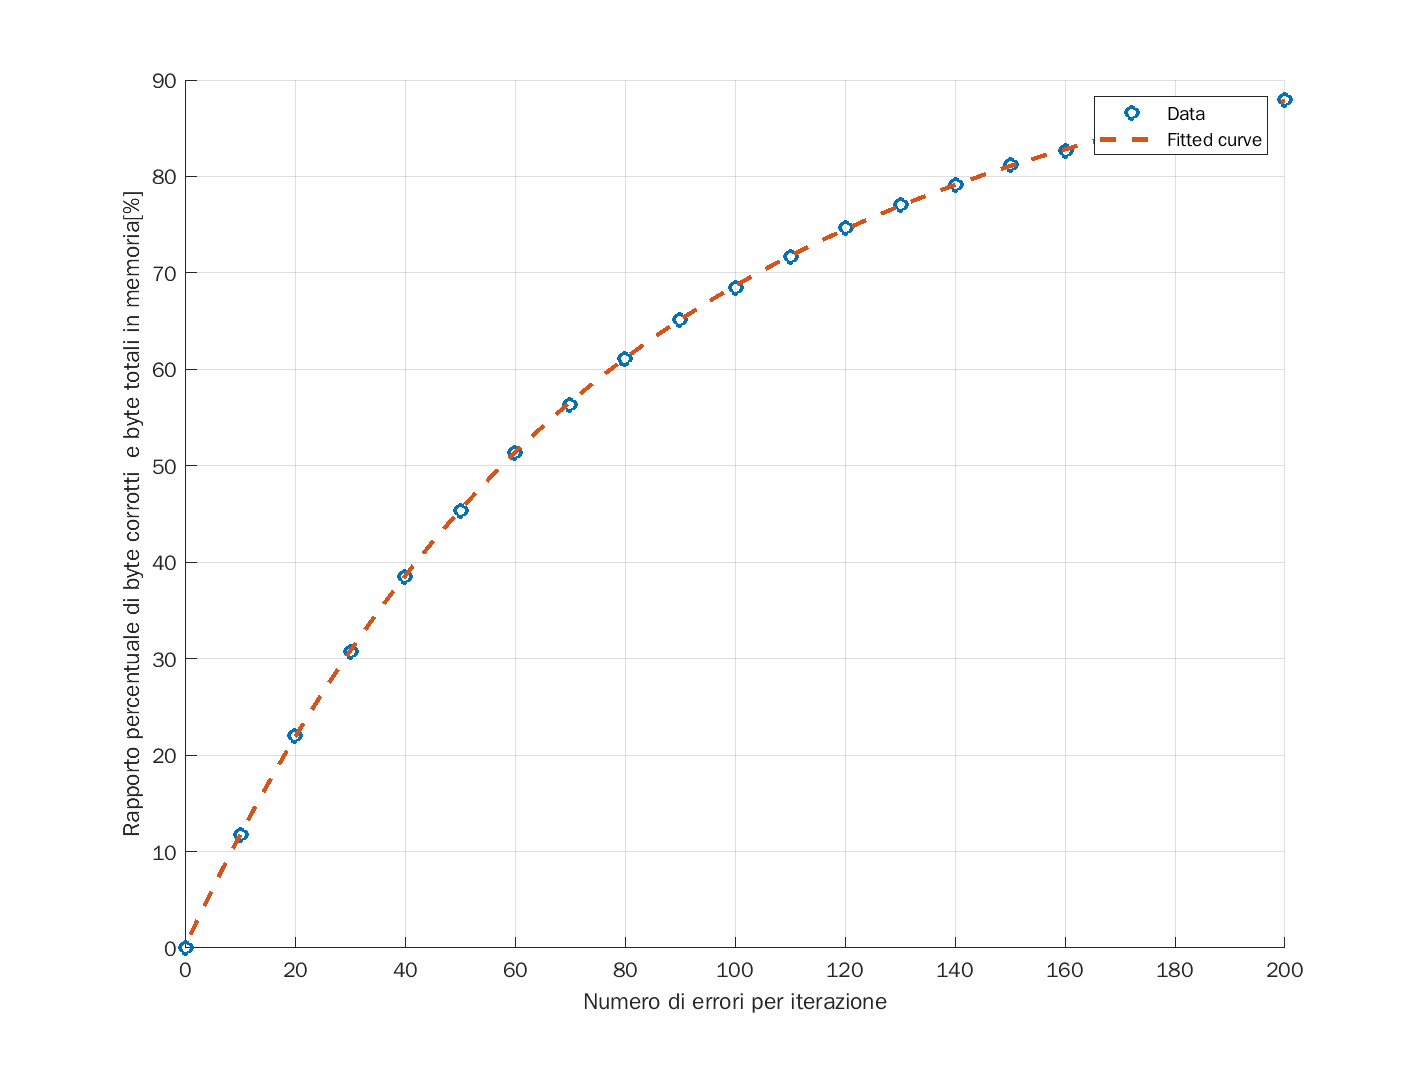
\includegraphics[scale=0.6]{examples/scrubbingTestParziali.png}}
\caption{la percentuale di byte errati del registro di stato in relazione al variare del numero di corruzioni.}
\label{fig}
\end{figure}
\vspace{0.5cm}
\newpage
\subsection{Codice sorgente riguardante il test di performance dell'algoritmo di scrubbing}
main.c:
\begin{lstlisting}[language=c][fontsize=\small]
#include <stdio.h>
#include <stdlib.h>
#include "scrub.h"
#include <time.h>
extern struct persistent_RAM persistent_RAM_;
extern struct persistent_RAM persistent_RAM_Copy_;
extern struct SatelliteStatus satelliteStatus_;


int main(int argc, char *argv[]) {
    srand(time(NULL));
    int nErrors = 0;
    int k;

    int iterations = 10;
    int errorPerIteration = 1;
    
    //EXAMPLE of input: ./main 100 3
    //number of iteration: 100
    //corruption per iteration: 3
    if(argv[1]!=0){
    	iterations = atoi(argv[1]);
    }
    if(argv[2]!=0){
    	errorPerIteration = atoi(argv[2]);
    }
    
    for(k=0;k<iterations;++k){
    
        initSatelliteStatus((uint8_t*)&satelliteStatus_.totalMissionMinutes, PERSISTENT_RAM_LENGTH);
        
        backupInPersistentRam (&persistent_RAM_.Memory[0],(uint8_t*)&satelliteStatus_.totalMissionMinutes,PERSISTENT_RAM_LENGTH);
        
        //This is a backup needed  for the oracol to detect any persistent corruption in satelliteStatus
        copyPersistentRamForFinalTest(&persistent_RAM_.Memory[0],&persistent_RAM_Copy_.Memory[0],PERSISTENT_RAM_LENGTH);
        
        setScrubParity(&persistent_RAM_.Memory[0],PERSISTENT_RAM_LENGTH/8);

        int i = 0 ;
        for(i = 0; i < errorPerIteration; ++i){
            insertSingleCorruption(&persistent_RAM_.Memory[0],PERSISTENT_RAM_LENGTH,0);
        }
        for(i = 0; i < errorPerIteration; ++i){
            insertSingleCorruption((uint8_t*)&satelliteStatus_.totalMissionMinutes,PERSISTENT_RAM_LENGTH,0);
        }
        scrub_recovery(&persistent_RAM_.Memory[0],PERSISTENT_RAM_LENGTH/8);
        if(scrub_recovery(&persistent_RAM_.Memory[0],PERSISTENT_RAM_LENGTH/8)==0){
            restoreFromPersistentRam(&persistent_RAM_.Memory[0],(uint8_t*)&satelliteStatus_.totalMissionMinutes,PERSISTENT_RAM_LENGTH);
        }else{
        }

        nErrors += numberOfErrors((uint8_t*)&satelliteStatus_.totalMissionMinutes);
    }

     float percentage = 100*(float)nErrors/(iterations*PERSISTENT_RAM_LENGTH);

	printf("%f\n",percentage);
	return 0;
	}
\end{lstlisting}

scrub.h:
\begin{lstlisting}[language=c][fontsize=\small]
#ifndef SCRUB_H_
#define SCRUB_H_


/*
 *
 * Funzione di calcolo della parità Verticale, genera un byte a partire da un blocco di otto byte
 *
*/


#include "scrub.h"
#include <stdint.h>
#define PERSISTENT_RAM_LENGTH 80
#define NUMBER_OF_EXPERIMENTS 6
#define PERSRAMMAGICWORD 0x07

struct parity
{
    int8_t h1[PERSISTENT_RAM_LENGTH/8];
    int8_t v1[PERSISTENT_RAM_LENGTH/8];
    int16_t d1[PERSISTENT_RAM_LENGTH/8];

    int8_t h2[PERSISTENT_RAM_LENGTH/8];
    int8_t v2[PERSISTENT_RAM_LENGTH/8];
    int16_t d2[PERSISTENT_RAM_LENGTH/8];
};

struct persistent_RAM
{
       uint8_t Memory[PERSISTENT_RAM_LENGTH];
};


struct SatelliteStatus
{

    uint32_t totalMissionMinutes;
    uint32_t timeAtBoot;

    uint8_t eventTest;
    uint16_t errors;
    uint8_t interruptCause;
    uint8_t isOnSun;
    uint32_t lastTimeOnSun;
    uint32_t lastTimeOnShadow;
    uint32_t lastTimeRTC;
    uint32_t lastTimeRTCunixTime;

    // Telemetry
    uint32_t telemetryLastTimeBeacon;
    uint32_t telemetryLastTimeTx;
    uint32_t telemetryLastTimeRead;
    uint32_t telemetryLastTimeSaved;

    // LABONCHIP
    uint8_t experimentRunning;
    uint8_t experimentEvent;
    uint8_t currentExperimentIndex;
    uint8_t currentExperimentStep;
    uint32_t startTimeCurrentExpStep;
    uint32_t expPauseInterval;

    // COMM
    uint16_t radioPacketIndex;
    uint16_t radioAckPacketIndex;
    uint32_t lastTimeRxGround;
    uint32_t lastTimeRadioReboot;
    uint16_t amateurPackets;
    uint16_t amateurTxPackets;

    //MEMORY
    uint8_t ignoreMemory;
};

int16_t Calc_VParity(int16_t Data[]);

int16_t Calc_HParity(int16_t Data[]);

int16_t Calc_DParity(int16_t Data[]);

int8_t scrubbing_bytes(int16_t Data[8],int8_t index);

void find_position(int16_t a, int16_t *ptr);

void initialize(int16_t *pt, int16_t size);

int16_t count_errors(int16_t a);

void toggle_bit(int16_t *pt,int16_t len,int16_t i,int16_t j);

void scrubbing_parity_generation(int16_t Data[8],int8_t stage,int8_t index );

void setScrubParity(uint8_t* index_pointer, uint8_t index_struct );

int8_t scrub_recovery(uint8_t* index_pointer, uint8_t index_struct );

void backupInPersistentRam (uint8_t* persistentStartingPointer,
                           uint8_t* memoryStartingPointer,
                           uint32_t length);
void restoreFromPersistentRam ( uint8_t* persistentStartingPointer,
                                uint8_t* memoryStartingPointer,
                                uint32_t length);
void printPersistentRam();

void printParity();

void insertSingleCorruption(unsigned char* startingPointer, unsigned int length, unsigned char log );

int numberOfErrors(uint8_t* startingPointer);


void initSatelliteStatus(uint8_t* startingPointer, uint32_t length);

void copyPersistentRamForFinalTest(uint8_t* startingPointer,uint8_t* copyStartingPointer, uint32_t length);

#endif /* SCRUB_H_ */
\end{lstlisting}


scrub.c:
\begin{lstlisting}[language=c][fontsize=\small]
#include "scrub.h"
#include <stdio.h>
#include <string.h>
#include <stdint.h>

struct persistent_RAM persistent_RAM_={0};
struct persistent_RAM persistent_RAM_Copy_={0};
struct parity parity_part={0};
struct SatelliteStatus satelliteStatus_={0};

int errori,correzioni = 0;


int16_t Calc_VParity(int16_t Data[])
{
    int16_t parity = 0;
    int16_t i;
    for(i=0; i<8; i++)
    {
        parity = parity ^ Data[i];
    }
    return parity;
}

int16_t Calc_HParity(int16_t Data[])
{
    int16_t parity = 0;
    int16_t temp;
    int16_t i,j, index;
    for(i=0; i<8; i++)
    {
        index = 0x80;
        temp = 0;
        for(j=0; j<8; j++)
        {
            if(Data[i] & index)
            {
                temp = temp ^ 0x0100;
            }
            index = index >> 1;
        }
        parity = parity ^ temp;
        parity = parity >> 1;
    }
    return parity;
}

int16_t Calc_DParity(int16_t Data[])
{
    int16_t parity = 0;
    int16_t dparity = 0;
    int16_t temp;
    int16_t i,j, index;
    for(i=0; i<8; i++)
    {
        index = 0x01;
        temp = 0;
        for(j=i; j>=0; j--)
        {
            if(Data[j] & index)
            {
                temp = temp ^ 0x0100;
            }
            index = index << 1;
        }
        parity = parity ^ temp;
        parity = parity >> 1;
    }

    for(i=1; i<=7; i++)
    {
        index = 0x80;
        temp = 0;
        for(j=i; j<=7; j++)
        {
            if(Data[j] & index)
            {
                temp = temp ^ 0x80;
            }
            index = index >> 1;
        }
        dparity = dparity ^ temp;
        dparity = dparity >> 1;
    }
    dparity = dparity << 8;
    dparity = dparity ^ parity;

    return dparity;
}



int8_t scrubbing_bytes(int16_t Data[8],int8_t index)
{
    int16_t h[8],v[8],d[16];
    int8_t dn, hn, vn;

    hn = count_errors(parity_part.h2[index] ^ parity_part.h1[index]);
    vn = count_errors(parity_part.v2[index] ^ parity_part.v1[index]);
    dn = count_errors(parity_part.d2[index] ^ parity_part.d1[index]);
    find_position(parity_part.h2[index] ^ parity_part.h1[index], h);
    find_position(parity_part.v2[index] ^ parity_part.v1[index], v);
    find_position(parity_part.d2[index] ^ parity_part.d1[index], d);

    if(hn==0 && vn==0 && dn==0)
    {
        return 0;
    }
    if((hn==1 && vn==1 && dn==1) && (d[0]==h[0]+v[0]))
    {
        toggle_bit(Data,8,h[0],v[0]);
    }
    if((hn==1 && vn==1 && dn==1) && (d[0]!=h[0]+v[0]))
    {
        if(d[0]<(h[0]+v[0]))
        {
            toggle_bit(Data,8,h[0],v[0]-1);
            toggle_bit(Data,8,h[0]-1,v[0]);
            toggle_bit(Data,8,h[0]-1,v[0]-1);
        }
        else
        {
            toggle_bit(Data,8,h[0],v[0]+1);
            toggle_bit(Data,8,h[0]+1,v[0]);
            toggle_bit(Data,8,h[0]+1,v[0]+1);
        }
    }
    if((hn==1 && vn==1 && dn==3) && (d[1]==h[0]+v[0]))
    {
    }
    if(hn==2 && vn==2 && dn==2)
    {
        if(d[0]==h[0]+v[0])
        {
            toggle_bit(Data,8,h[0],v[0]);
            toggle_bit(Data,8,h[1],v[1]);
        }
        else
        {
            toggle_bit(Data,8,h[1],v[0]);
            toggle_bit(Data,8,h[0],v[1]);
        }
    }
    if(hn==0 && vn==2 && dn==2)
    {
        toggle_bit(Data,8,(d[0]-v[0]),v[0]);
        toggle_bit(Data,8,(d[1]-v[1]),v[1]);
    }
    if(hn==2 && vn==0 && dn==2)
    {
        toggle_bit(Data,8,h[0],(d[0]-h[0]));
        toggle_bit(Data,8,h[0],(d[1]-h[1]));
    }
    if(hn==2 && vn==2 && dn==0)
    {
        toggle_bit(Data,8,h[0],v[1]);
        toggle_bit(Data,8,h[1],v[0]);
    }
    if(hn==1 && vn==3 && dn==3)
    {
        toggle_bit(Data,8,h[0],v[0]);
        toggle_bit(Data,8,h[0],v[1]);
        toggle_bit(Data,8,h[0],v[2]);
    }
    if(hn==3 && vn==1 && dn==3)
    {
        toggle_bit(Data,8,h[0],v[0]);
        toggle_bit(Data,8,h[1],v[0]);
        toggle_bit(Data,8,h[2],v[0]);
    }
    if(hn==3 && vn==3 && dn==1)
    {
        toggle_bit(Data,8,h[2],v[0]);
        toggle_bit(Data,8,h[1],v[1]);
        toggle_bit(Data,8,h[0],v[2]);
    }
    if(hn==3&&vn==3&&dn==3&&(d[0]==h[0]+v[0])&&(d[1]==h[1]+v[1])&&(d[2]==h[2]+v[2]))
    {
        toggle_bit(Data,8,h[0],v[0]);
        toggle_bit(Data,8,h[1],v[1]);
        toggle_bit(Data,8,h[2],v[2]);
    }

    return 1;
}

void find_position(int16_t a, int16_t *ptr)
{
    int16_t i;
    int16_t index = 1;
    for(i=0; i<16; i++)
    {
        if(a & index)
        {
            *ptr=i;
            ptr++;
        }
        index = index <<1;
    }
}
void initialize(int16_t *pt, int16_t size)
{
    int16_t i;
    for(i=0; i<size; i++)
    {
        *pt=-1;
        pt++;
    }
}
int16_t count_errors(int16_t a)
{
    int16_t i;
    int16_t index = 1;
    int16_t count = 0;

    for(i=0; i<16; i++)
    {
        if(a & index)
        {
            count=count+1;
        }
        index = index <<1;
    }
    return count;
}


void toggle_bit(int16_t *pt,int16_t len,int16_t i,int16_t j)
{
    if(i<len)
    {
        pt[i] ^= 1UL << (j);
    }
}

void scrubbing_parity_generation(int16_t Data[8],int8_t stage,int8_t index )
{
    int16_t h[8],v[8],d[16];

    initialize(h,8);
    initialize(v,8);
    initialize(d,16);
    if(stage == 0)
    {

        parity_part.h1[index]=Calc_HParity(Data);
        parity_part.v1[index]=Calc_VParity(Data);
        parity_part.d1[index]=Calc_DParity(Data);

    }
    else if (stage == 1)
    {
        parity_part.h2[index]=Calc_HParity(Data);
        parity_part.v2[index]=Calc_VParity(Data);
        parity_part.d2[index]=Calc_DParity(Data);
    }
    else
    {

    }
}

void setScrubParity( uint8_t* index_pointer, uint8_t index_struct )
{
    uint8_t i,j;
    uint8_t *pointer = (uint8_t*)index_pointer;
    for ( i = 0; i<index_struct ; ++i){
        int16_t Data_memory_control[8]={0};
        for ( j=0; j<8; j++ )
        {
            Data_memory_control[j]=(int16_t)*pointer;
            pointer++;
        }
        scrubbing_parity_generation(Data_memory_control,0,i);
    }
}

int8_t scrub_recovery( uint8_t* index_pointer, uint8_t index_struct )
{
    uint8_t i,j;
    uint8_t return_value=0;
    uint8_t *pointer;
    int16_t Data_memory_control[8];
    pointer=(uint8_t*)(index_pointer);
    for ( i = 0; i<index_struct ; ++i){
        for ( j=0; j<8; j++ )
        {
            Data_memory_control[j]=pointer[8*i+j];
        }
        scrubbing_parity_generation(Data_memory_control,1,i);
        int result = scrubbing_bytes(Data_memory_control,i);
        if(result==1)
        {

            for ( j=0; j<8; j++ )
            {

                pointer[j+8*i]=Data_memory_control[j];
            }
            //++correzioni;
            return_value+=1;
        }
        else if(result==2){
            //++errori;
        }
        else if(result==0){
            //printf("Tutto bene\n");
        }
    }

    //printf("Correzioni: %d",correzioni);
    //printf("Errori:     %d",errori);
    return return_value;
}




void backupInPersistentRam (uint8_t* persistentStartingPointer,
        uint8_t* memoryStartingPointer,
        uint32_t length){
    int i  = 0;
    for (  i = 0 ; i<length; ++i){
        persistentStartingPointer[i]=memoryStartingPointer[i];
    }
}


void restoreFromPersistentRam (uint8_t* persistentStartingPointer,
        uint8_t* memoryStartingPointer,
        uint32_t length){
    int i = 0;
    for (  i = 0 ; i<length; ++i){
        memoryStartingPointer[i]=persistentStartingPointer[i];
    }
}
void printPersistentRam(){
    int i  = 0;
    for ( i = 0 ; i<PERSISTENT_RAM_LENGTH; ++i){
        printf("Elemento: %x\n",persistent_RAM_.Memory[i]);
    }

}

void printParity(){
    uint32_t l;

    for (l = 0; l < PERSISTENT_RAM_LENGTH/8; l++)
    {
        printf("h1:%x\tv1:%x\td1:%x_____",parity_part.h1[l],
                parity_part.v1[l],parity_part.d1[l]);
        printf("h2:%x\tv2:%x\td2:%x\n",parity_part.h2[l],
                parity_part.v2[l],parity_part.d2[l]);
    }
    printf("___________________________________\n");



}

void insertSingleCorruption(unsigned char* startingPointer, unsigned int length, unsigned char log ){
    unsigned int arrayIndex = rand() % length;
    unsigned int byteIndex = rand() % 8;
	    if(log!=0){
	    printf("Location %d before the corruption was: 0x%x\n",arrayIndex,startingPointer[arrayIndex]);
	    }
    startingPointer[arrayIndex] = startingPointer[arrayIndex] ^ ( 1 << byteIndex );
	    if(log!=0){
	    printf("Location %d after the corruption was: 0x%x\n",arrayIndex,startingPointer[arrayIndex]);
	    }
}

int numberOfErrors(uint8_t* startingPointer){
    int result = 0;
    int i;
    for (i=0;i<PERSISTENT_RAM_LENGTH;++i){
        if(startingPointer[i]!=persistent_RAM_Copy_.Memory[i]){
            ++result;
        }
    }
    return result;
}

void initSatelliteStatus(uint8_t* startingPointer, uint32_t length){
    uint32_t i;
    for ( i = 0; i<length;++i ){
        startingPointer[i]=(uint8_t)rand();
    }
}

void copyPersistentRamForFinalTest(uint8_t* startingPointer,uint8_t* copyStartingPointer, uint32_t length){
    uint32_t i;
    for ( i = 0; i<length;++i ){
        copyStartingPointer[i]=startingPointer[i];
    }
}
\end{lstlisting}

\subsection{Iniezione di corruzioni nella sezione di "Persistent" nel sistema Abacus}

Il test di integrazione dell'algoritmo di scrubbing su un sistema microcontrollore è consistito nella corruzione di una locazione casuale di una parte di memoria persistent RAM, copia di una sezione di memoria RAM utilizzata dal microcontrollore. 
Questa parte di memoria definita come backup di dati utilizzati dal sistema è generica. In una situazione pratica questa parte di memoria coinciderebbe con lo spazio di memoria occupato dal registro di stato del satellite.

L'obiettivo finale di questo test è stato verificare la correzione sia della parte persistent che del buffer di memoria utilizzato, preventivamente corrotti manualmente.

La prima azione che l'algoritmo di scrubbing si è occupato di fare è il backup dell'informazione contenuta nella memoria utilizzata dal sistema all'interno della parte persistent (la memoria di backup protetta appunto dallo scrubbing). Questo meccanismo è necessario poiché il contenuto informativo di sezioni dati di zona di memoria come il registro di stato è soggetto a variazioni periodiche e non continue (come ad esempio il numero di rebbot che il microcontrollore esegue). 

Nel caso in cui il microcontrollore sia costretto a eseguire un reset del sistema l'informazione nella registro di stato sarebbe persa. Questo poichè la memoria RAM generica è una memoria volatile. Dunque avere un backup periodico del registro di stato è molto utile per poter ripartire da una situazione non di partenza.

La figura 4.6 descrive la struttura dati utilizzata per simulare una generica parte di memoria chiamata per l'appunto Memory. Questa consiste in un buffer di valori unsigned char e a partire da questa l'algoritmo eseguirà un backup nella parte persistent di memoria.
\begin{figure}[htbp]
\centerline{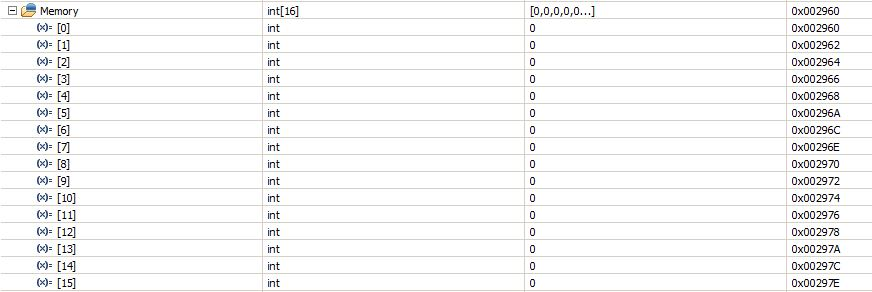
\includegraphics[scale=0.6]{examples/1_MemoryNonCorrottaInizio.JPG}}
\caption{I valori contenuti all'interno della memoria su cui eseguire il backup in persistent RAM.}
\label{fig}
\end{figure}
\newline
L'azione che viene eseguita periodicamente è quella di salvare i valori contenuti nella Memory all'interno della zona persistent (vedi figura 4.7), ovvero una struttura che contiene sia una copia della struttura dati originale, la parte di ridondanza che descrive la "Parità 4d" ed infine una flag che discrimina se la memoria persistent è stata già scritta almeno per una volta ed in questo modo evita eventuali restore di valori non corretti all'interno della memoria originale.

\begin{figure}[htbp]
\centerline{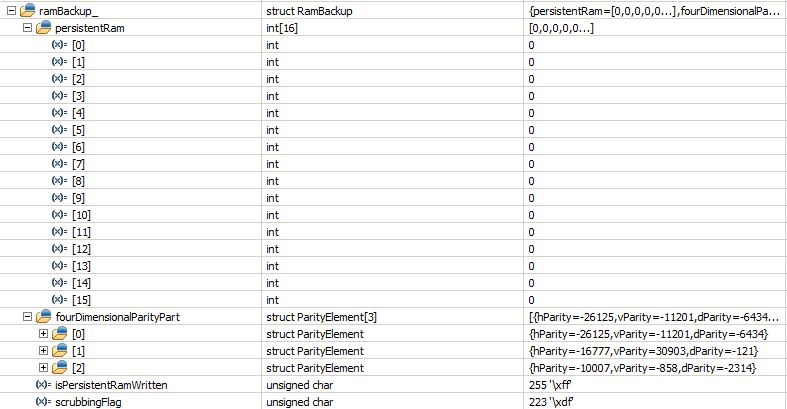
\includegraphics[scale=0.6]{examples/2_PersistentRamBackup.JPG}}
\caption{La struttura di backup del registro di stato del satellite in persistent RAM}
\label{fig}
\end{figure}
\vspace{0.5cm}

Utilizzando il Memory Browser, vedi figura 4.8, abbiamo corrotto una locazione di memoria della RAM originale. Questa operazione è facilmente eseguibile in fase di Debug premendo direttamente su una locazione a scelta (nel nostro caso quella evidenziata in blu). Una volta scritto un valore e premuto invio, la modifica risulta consistente anche all'interno della memoria fisica e dunque è possibile eseguire la corruzione della memoria originale.

\begin{figure}[htbp]
\centerline{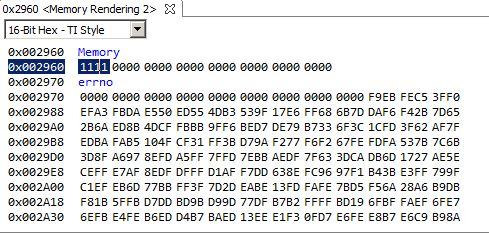
\includegraphics[scale=0.8]{examples/3_MemoryBrowserCorruzione.JPG}}
\caption{Corruzione della memoria principale.}
\label{fig}
\end{figure}
\vspace{0.5cm}

Utilizzando la stessa metodologia, ma cambiando il valore di partenza di locazione di memoria da poter consultare tramite il Memory Browser (modificabile dal menu in alto che attualmente punta alla locazione 0x2960), abbiamo corrotto anche una locazione della persistent RAM. 
Questa è proprio la zona di memoria di backup che tramite l'algoritmo di scrubbing viene periodicamente pulita da eventuali corruzioni. L'obiettivo di questo test sarà dunque il riscontro della correzione della persistentRAM e conseguentemente la riscrittura di essa sulla memoria principale.
\begin{figure}[htbp]
\centerline{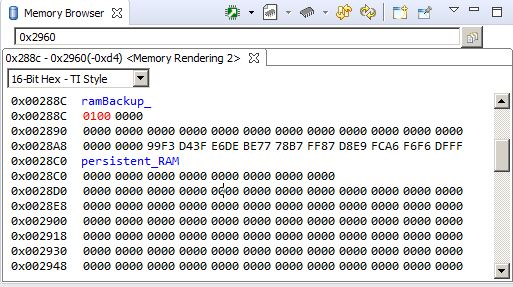
\includegraphics[scale=0.8]{examples/5_PersistentRamCorruzione.JPG}}
\caption{Corruzione della memoria persistentRam.}
\label{fig}
\end{figure}
\newline
In fase di esecuzione scatta dunque periodicamente l'algoritmo di scrubbing, il quale si occupa di rivelare e possibilmente correggere le sezioni di memoria corrotte. Nel nostro caso il primo gruppo di byte è proprio il settore da correggere, mentre gli altri sono riconosciuti come sezioni corrette. Come è possibile notare dalla figura 4.10, il valore 0x1000 viene correttamente riscritto al suo valore originale (nel nostro caso era proprio 0x0000)

\begin{figure}[htbp]
\centerline{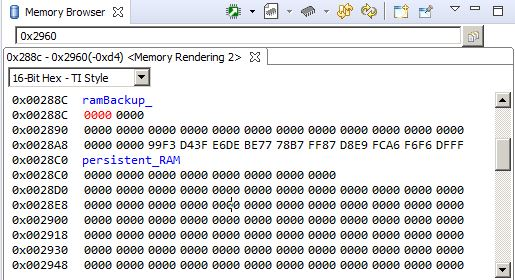
\includegraphics[scale=0.8]{examples/6_ScrubbingPersistentRamRiuscita.JPG}}
\caption{Correzione tramite l'algoritmo di scrubbing della memoria di scrubbing.}
\label{fig}
\end{figure}
\vspace{0.5cm}

Infine il codice di scrubbing si occupa di ripristina il valore in persistent RAM direttamente nella memoria principale.
Le due condizioni necessarie per il ripristino sono:
\begin{itemize}
    \item Che la flag chiamata "isPersistentRamWritten" sia già stata alzata, dunque che il contenuto della persistentRAM contenga almeno un backup.
    
    \item Che la parità 4D salvata in memoria sia coincidente con quella calcolata durante il controllo. Questo significa che il contenuto di backup sia completamente integro.
    
\end{itemize}
Nella figura 4.11 andiamo dunque ad analizzare il contenuto della memoria principale (sita nel nostro caso nella locazione 0x2960). I valori corrotti sono stati dunque ripristinati e l'integrità della memoria è stata conservata.
\begin{figure}[htbp]
\centerline{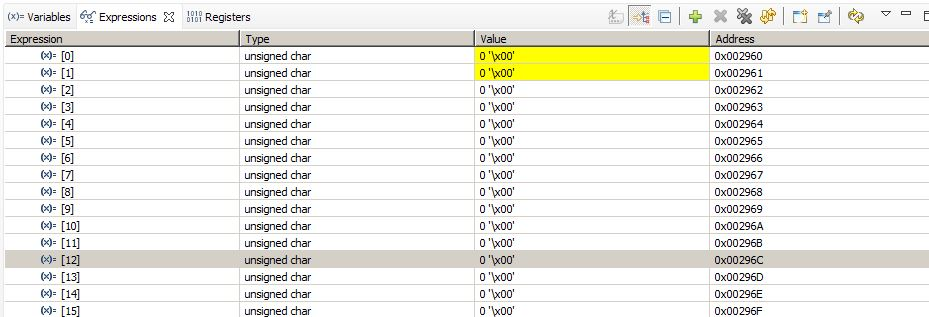
\includegraphics[scale=0.6]{examples/7_CorrezioneMemory.JPG}}
\caption{Correzione della memoria principale tramite i valori presenti in persistentRam.}
\label{fig}
\end{figure}
\vspace{0.5cm}

\chapter{Autodiagnosi delle componenti del microcontrollore/FPGA MSP430}

Il sistema di Abacus permette anche in fase di esecuzione di disattivare o attivare la comunicazione con alcune parti dell’hardware senza inficiare direttamente sul corretto funzionamento del satellite. 
Questa caratteristica è molto utile in un ambiente in cui alcuni componenti possono essere ad esempio danneggiate da agenti esterni come radiazione o da detriti e oltretutto non possono essere direttamente riparati durante il volo. 

L’obiettivo dunque dell’algoritmo nel caso del controllo dei sensori è quello di testare individualmente ogni singola componente hardware facendolo interrogare dalla CPU tramite il corretto protocollo di comunicazione.


\section{Architettura Hardware e protocolli di comunicazione in Abacus}

Come si evince dalla figura 6.2, la comunicazione con il microcontrollore e i sensori avviene tramite protocollo I2C.
Per quanto riguarda sia la memoria Flash del microcontrollore ("MCU Flash") che la memoria Flash dell'FPGA ("FPGA Flash") il microcontrollore utilizza il protocollo SPI per comunicare con entrambe le memorie. Anche in questo caso nelle memorie sono definiti dei registri (3 in entrambi i casi) in cui viene definito un valore di ID e di conseguenza la modalità di controllo è la stessa utilizzata per i sensori.

Analizziamo dunque come è formato il pacchetto SPI ricevuto:
\begin{itemize}
    \item Byte 0: Protocol (1) - la costante che definisce la "data  operation" è pari a 1.
    
    \item Byte 1: Opcode
    
    \item Bytes 2 - 3: Request ID - Request ID associato alla risposta e al NAKs (negative acknowledgements) con la richiesta. Il microcontrollore dovrebbe eseguire una richiesta alla volta data la natura del protocollo.
\end{itemize}
    

\begin{figure}[htbp]
\centerline{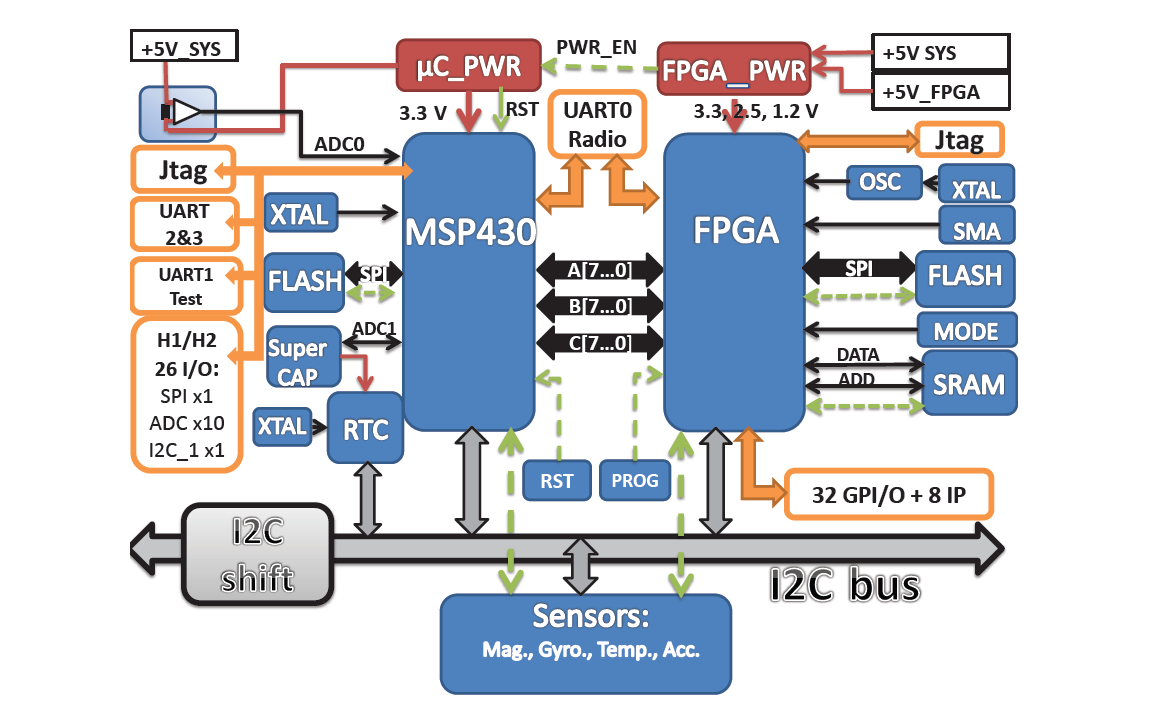
\includegraphics[scale=0.6]{examples/ABACUS_overview.png}}
\caption{Rappresentazione grafica dell'algoritmo di controllo di parità quadridimensionale}
\label{fig}
\end{figure}
\vspace{0.5cm}

\section{Architettura dei diversi sottosistemi hardware}



Ogni versione di Abacus ha a disposizione diversi componenti hardware ma il numero dei sensori è rimasto inalterato nel tempo.
Di seguito è possibile consultare i valori dei registri necessari per il controllo. Tale costanti sono specificate per tutte e tre le diverse versioni di abacus disponibili ad oggi:

\begin{figure}[htbp]
\centerline{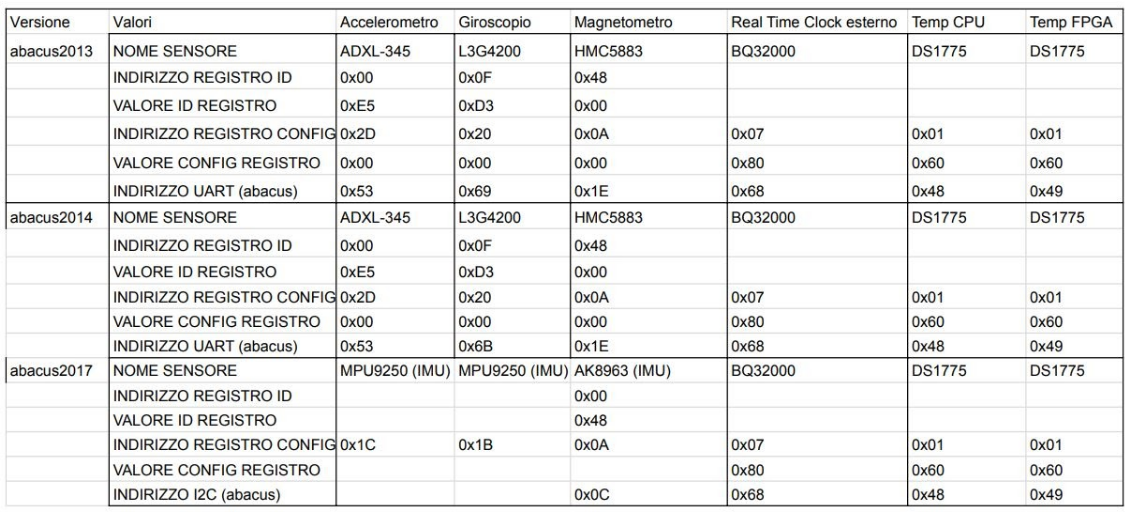
\includegraphics[scale=0.55]{examples/registerMapSensori.PNG}}
\caption{Elenco dei dei registri di ogni sensore che il MCU interroga}
\label{fig}
\end{figure}
\vspace{0.5cm}

La struttura dell'algoritmo è dunque utilizzabile per tutte le diverse versioni di Abacus.
Il codice utilizza ovviamente una delle tre configurazioni in armonia con l'impostazione del sistema (nei nostri test è stata utilizzata la versione 2017). Per utilizzare una versione differente basta cambiare le costanti che l'algoritmo e tali valori sono già presenti nel file header.


\section{Struttura del codice di autodiagnosi}

L’obiettivo dunque dell’algoritmo di diagnosi dei sensori è quello di testare individualmente ogni singola componente hardware, interrogandola tramite il corretto protocollo di comunicazione.
Nel caso dei sensori la corretta comunicazione avviene tramite protocollo I2C e di conseguenza il corretto funzionamento è garantito tramite l’azione di richiedere il numero identificativo specifico (chiamato “Device ID”), ovvero un valore costante definito all’interno di uno dei registri del satellite. Una volta richiesto tale valore, il sensore se funzionante dovrebbe rispondere in un tempo limitato. Per garantire ciò la cpu imposta un timer software e dunque un timeout per la risposta. Questo garantisce che la comunicazione tra microcontrollore ed il sensore è definita correttamente.

Una volta ricevuto il messaggio di risposta contenente il device ID, basterà confrontarlo con il valore definito a priori all’interno del microcontrollore. Se i due valori sono coincidenti, il valore contenuto all’interno del registro del sensore è corretto (dunque non corrotto) e conseguentemente la comunicazione hardware-microcontrollore è svolta in maniera coerente. In secondo luogo, è possibile verificare le corrette impostazioni dei sensori, analizzando e correggendo se necessario i registri di configurazione (uno o più in base al tipo di sensore). 

Il meccanismo di timeout della comunicazione è quindi non più utilizzato poiché arrivati a questo punto, siamo certi di comunicare con il sensore.
Ogni malfunzionamento (del singolo sensore o dell'intero bus I2C) è gestito in maniera diversa in base alla tipologia ed importanza di ogni singolo sensore.

La funzione di controllo dello stato del sensore infatti fornisce come valore di ritorno un valore pari a 0 nel caso in cui tutto funzioni correttamente, mentre un valore maggiore di 0 nel caso in cui abbia evidenzia una incorrettezza.

Questo valore di ritorno sarà dunque sommato per tutti i sensori di Abacus e la somma fornirà l'entità del problema. E' stata dunque stabilità una soglia minima (pari al valore esadecimale 0x10) per cui il sistema eseguirà subito un software reset.

Come altra contromisura sono state definite delle flag salvati nella zona di memoria definite come "Persistent" (definite a partire dallo stesso meccanismo utilizzato nel caso dell'algoritmo di scrubbing) e dunque consultabile anche dopo un software reset, in modo da escludere direttamente al nuovo riavvio l'utilizzo del sensore danneggiato evitando così un errato utilizzo delle periferiche malfunzionanti. 

Questo  meccanismo è molto utile per mantenere memoria dello stato del satellite ed evitare dunque un ricontrollo di un componente sicuramente non funzionante.
\newline\newline
Lo stesso funzionamento è replicato nel caso del controllo delle memorie flash esterne al microcontrollore, poiché anche questi hardware hanno dei registri specifici di identificazione i quali possono essere consultati tramite protocollo SPI.

\begin{figure}[htbp]
\centerline{\includegraphics[scale=0.43]{examples/corruptionCheckAsm.PNG}}
\caption{Diagramma di flusso dell'algoritmo di autodiagnosi. Il controllo di integrità è eseguito su tutti i componenti hardware definiti, ma il grafico ne evidenzia soltanto due per semplificazione grafica.}
\label{fig}
\end{figure}


\clearpage
\subsection{Codice sorgente dell'algoritmo di autodiagnosi}
Di seguito è fornito l'implementazione dell'algoritmo di autodiagnosi in codice C:

selfDiag.h:
\begin{lstlisting}[language=c][fontsize=\small]
#ifndef INCLUDE_SELFDIAG_H_
#define INCLUDE_SELFDIAG_H_
#include "abacus.h"

//Accelerometro
//abacusversion2013 and abacusversion2014
#define AB_ADDRESS_ACC_ID               0xE5
#define ADXL345_STD_CONFIG              0x00
#define ADXL345DEVID                    0x00
//abacusversion2017
#define MPU9250_IMU_ID			0x71
#define MPU9250_ACC_STD_CONFIG		0x00	


//Giroscopio
//abacusversion2013 and abacusversion2014
#define AB_ADDRESS_GYR_ID               0xD3
#define L3G4200_DEVID                   0x0F
#define L3G4200_STD_CONFIG              0x00
//abacusversion2017 lo stesso dell'accelerometro
#define MPU9250_GYR_STD_CONFIG		0x00


//Magnetometro
//abacusversion2013 and abacusversion2014
#define HMC5883_DEVID                   0x48   
#define HMC5883_STD_CONFIG              0x00
#define HMC5883IDREG_A                  0x0A
//abacusversion2017
#define AK8963_DEVID                   0x48
#define AK8963_STD_CONFIG              0x00


//RTC (Real Time Clock)
#define BQ32000_STD_CONFIG              0x80
#define BQ32000CAL_CFG1                 0x07
//CPU temp sensor
#define DS1775_CPU_STD_CONFIG           0x60

//FPGA temp sensor
#define DS1775_FPGA_STD_CONFIG          0x60


//Codifica della priorità di autodiagnosi
// Il byte che manterrà l'informazione ha dunque la seguente struttura:
//  0b xxxx xxxx ---> Ogni singolo bit (tranne il secondo che non è utilizzato) avrà la seguente logica:
//                    0 -> Sensore funzionante
//                    1 -> Sensore non funzionante
//

#define AUTO_I2C_RETURN_VALUE           0x80

#define AUTO_FPGA_TEMP_RETURN_VALUE     0x20
#define AUTO_CPU_TEMP_RETURN_VALUE      0x10
#define AUTO_RTC_RETURN_VALUE           0x08
#define AUTO_MAG_RETURN_VALUE           0x04
#define AUTO_GYR_RETURN_VALUE           0x02
#define AUTO_ACC_RETURN_VALUE           0x01


//Valori di identificazione della memoria flash
#define FLASH_IDEN_BYTE_0 0x20
#define FLASH_IDEN_BYTE_1 0x20
#define FLASH_IDEN_BYTE_2 0x18


//#pragma PERSISTENT(PersistentRam)
struct DiagnosticFlags
{
        uint8_t I2CFlag;                           
        uint8_t accelerometerSensorFlag;
        uint8_t gyroscopeSensorFlag;
        uint8_t magnetometerSensorFlag;
        uint8_t fpgaTemperatureSensorFlag;

        uint8_t cpuTemperatureSensorFlag;
        uint8_t rtcFlag;
        uint8_t flashFlag;
        uint8_t fpgaTemperatureSensorSecondFlag;
        uint8_t cpuTemperatureSensorSecondFlag;		
}diagnosticFlags;

uint8_t     checkAccelerometerId(uint8_t* flag);
uint8_t     checkGyroscopeId(uint8_t* flag);
uint8_t     checkMagnetometerId(uint8_t* flag);
uint8_t     checkRtcId(uint8_t* flag);
uint8_t     checkTempCpuId(uint8_t* flag);
uint8_t     checkTempFpgaId(uint8_t* flag);

void controlIntegrity(uint32_t timeInterval);


//Funzionne di controllo della memoria flash
void        checkFlashMemoryId(uint8_t* flag);


/*Funzione che permette di valutare la maggioranza di 0 o 1 all'interno di un byte.
* In questo la corruzione di pochi bit non inficia sulla valutazione del valore della flag
*
* Esempio:
* Flag_x=0xff;   => 0b 1111 1111
* Tramite una corruzione vedo:
* Flag_x=0x3f;   => 0b 0011 1111
* La funzione decide per flag=1 correttamente
* soltanto 5 corruzione o pi� di fatto mi danno un valore sbagliato.
*
*/
uint8_t     majorityDecisionByte(uint8_t value);


void sensorDiag(void);
void memoryDiag(void);

int8_t selfDiagInit();





#endif /* INCLUDE_SELFDIAG_H_ */
\end{lstlisting}


selfDiag.c:
\begin{lstlisting}[language=c][fontsize=\small]
#include "selfDiag.h"
#include "abacus.h"


/*
 * Quelle flag riferite ad ogni parte dell'hardware definite come persistent
 * ci permettono di monitorare anche dopo un reset l'effettivo funzionamento.
 * flag=0 significa funzionante
 * flag=1 significa da escludere direttamente all'avvio
 *
 */


uint8_t     majorityDecisionByte(uint8_t value){
    uint8_t result = 0;
    uint8_t counter = 0;
    uint8_t bit = 0;
    uint8_t mask;
    uint8_t i;
    for(i=0;i<8;++i) {
        mask = 1<<i;
        bit = value & mask;
        if( bit != 0x0 ) {
            ++counter;
        }
    }
    if(counter>3){
        result = 0xff;
    }
    return result;
}

/*raises flag for non functional sensors*/
void sensorDiag(void)
{
    uint8_t counter=0;
    if ( majorityDecisionByte(diagnosticFlags.I2CFlag) == 0x0 )
    {


        // Prima di controllare ogni singolo sensore, ad ogni iterazione si esegue un controllo sul bus I2C condiviso tra tutti i sottosistemi interrogati.
        // Questo evita il ricontrollo del bus I2C e di conseguenza un possibile overflow al contatore (verrebbe sommato per n volte 0x80
        // Evito per sicurezza il controllo dei sensori e li disabilito a priori nel caso in cui il bus non sia funzionante

        if( ( majorityDecisionByte(diagnosticFlags.accelerometerSensorFlag) == 0x0) )
        {
            counter+=checkAccelerometerId(&diagnosticFlags.accelerometerSensorFlag);
        }
        else
        {
            //Se riscontro un flag alta, per sicurezza escludo il sensore
            abacus_sensors_acc_power_off();
        }


        /********************/
        if( (majorityDecisionByte(diagnosticFlags.gyroscopeSensorFlag)==0x0) )
        {
            counter+=checkGyroscopeId(&diagnosticFlags.gyroscopeSensorFlag);
        }
        else
        {
            abacus_sensors_gyro_power_off();
        }

        /*******************/
        if( ( majorityDecisionByte(diagnosticFlags.magnetometerSensorFlag)==0x0)  && ( majorityDecisionByte(diagnosticFlags.I2CFlag) == 0x0 ) )
        {
            counter+=checkMagnetometerId(&diagnosticFlags.magnetometerSensorFlag);
        }
        else
        {
            abacus_sensors_magnetometer_power_off();
        }
        /*******************/
        if( ( majorityDecisionByte(diagnosticFlags.cpuTemperatureSensorFlag)==0x0)  && ( majorityDecisionByte(diagnosticFlags.I2CFlag) == 0x0 ) )
        {
            counter+=checkTempCpuId(&diagnosticFlags.cpuTemperatureSensorFlag);
        }
        else
        {
            if( (majorityDecisionByte(diagnosticFlags.cpuTemperatureSensorSecondFlag)==0x0)  && ( majorityDecisionByte(diagnosticFlags.I2CFlag) == 0x0 ) )
            {
                counter+=checkTempCpuId(&diagnosticFlags.cpuTemperatureSensorSecondFlag);
            }
            else
            {
                abacus_sensors_temperatureCPU_power_off();
            }
        }
        /********************/
        if( ( majorityDecisionByte(diagnosticFlags.fpgaTemperatureSensorFlag)==0x0) && ( majorityDecisionByte(diagnosticFlags.I2CFlag) == 0x0 ) )
        {
            counter+=checkTempFpgaId(&diagnosticFlags.fpgaTemperatureSensorFlag);
        }
        else
        {
            if( ( majorityDecisionByte(diagnosticFlags.fpgaTemperatureSensorSecondFlag)==0x0) && ( majorityDecisionByte(diagnosticFlags.I2CFlag) == 0x0 ) )
            {
                counter+=checkTempFpgaId(&diagnosticFlags.fpgaTemperatureSensorSecondFlag);
            }
            else
            {
                abacus_sensors_temperatureFPGA_power_off();
            }
        }

        if( ( majorityDecisionByte(diagnosticFlags.rtcFlag)==0x0) && ( majorityDecisionByte(diagnosticFlags.I2CFlag) == 0x0 ) )
        {
            counter+=checkRtcId(&diagnosticFlags.rtcFlag);
        }
    }
    else
    {
        counter = 0xff;
        diagnosticFlags.accelerometerSensorFlag = 0xff;
        diagnosticFlags.I2CFlag = 0xff;
        diagnosticFlags.accelerometerSensorFlag  = 0xff;
        diagnosticFlags.gyroscopeSensorFlag  = 0xff;
        diagnosticFlags.magnetometerSensorFlag = 0xff;
        diagnosticFlags.fpgaTemperatureSensorFlag  = 0xff;
        diagnosticFlags.cpuTemperatureSensorFlag = 0xff;
        diagnosticFlags.rtcFlag = 0xff;
        diagnosticFlags.fpgaTemperatureSensorSecondFlag = 0xff;
        diagnosticFlags.cpuTemperatureSensorSecondFlag = 0xff;
    }

    if(counter > 0x8)
    {                                             
        WDTCTL = 0xDEAD;
    }


}


/*check for the memory issues and implement appropriate routines*/
void memoryDiag(void)
{
    //Da completare
    if(majorityDecisionByte(diagnosticFlags.flashFlag)==0x0)
    {
        checkFlashMemoryId(&diagnosticFlags.flashFlag);
    }

}

/*
 * Ogni richiesta di controllo del determinato sensore avviene tramite protocollo I2C. Questo protocollo si svolge in due parti: prima si richiede la determinata risorsa, poi il sensore ris
 * ponde alla determinata richiesta. Ci� non avviene sempre e qualcosa pu� andare storto (sensore rotto, bus I2C non funzionante). Per evitare che il codice si blocchi imponiamo quindi un
 * tempo limite di risposta, pari ad un numero precisato di operazioni. Se il contatore raggiunge il limite, significa che il bus non risponde e di conseguenza bisogna supporre che entrambe
 * le risorse (sensore e bus) non sono utilizzabili. In tal caso le flag a byte rimangono alte e dopo un software reset obbligato le risorse vengono escluse o il problema viene risolto.
 * Come ultima spiaggia abbiamo inoltre attivato il watchdog timer che ci permette di non bloccare il codice nel caso in cui tutta la procedura venga bloccata da un evento inaspettato.
 *
 *
 *
 */
uint8_t checkAccelerometerId(uint8_t* flag)
{



    //WDTCTL = (WDTCTL & 0x00FF) | WDTPW | WDTCNTCL;
    *flag=0xFF;
    diagnosticFlags.I2CFlag=0xFF;

    uint8_t counter=0;
    uint8_t result=0;

    /*
     **  Una volta appurato che il bus I2C risponde e ci fornisce la determinata risorsa, bisogna valutare che i registri non siano corrotti.
     **  Per Fare ci� vi � un registro dedicato nella maggior parte dei sensori chiamato "Device ID" che ci permette di leggere il nome del sensore.
     **  Se ci� non avviene correttamente, il registro � corrotto.
     **  Nel caso in cui il registro non sia corrotto andiamo poi ad indagare il registro di configurazione, il quale deve essere impostato secondo un determinato valore
     **  esadecimale (gi� deciso a priori). Se ci� non avviene significa che qualcosa � cambiato e ci� � inaspettato.
     **  In tale caso, andiamo a resettare le impostazioni del sensore.
     **
     **  SINTASSI DELLA RICHIESTA I2C DI LETTURA DI UN REGISTRO:
     **    while(uint8_t abacus_i2c_readRegister(uint8_t busSelect,uint8_t address, uint8_t reg)
     */


    while( ( result = abacus_i2c_readRegister(AB_I2C_BUS00, AB_ADDRESS_ACC, ADXL345DEVID) ) == 0x00)
    {
        counter++;

        if(counter > 30000)             //i2c is not responding, power reset, so i both acc and i2c not working to be sure
        {
            result = AUTO_ACC_RETURN_VALUE+AUTO_I2C_RETURN_VALUE;
            /*
             *
             * Il valore dipende dalla priorit� con cui bisogna risolvere il problema: questo identifica che sia il bus IC che l'accelerometro sono non funzionanti:
             *
             * 0b1000 0000 + 0b0000 0001 = 0b1000 0001 = 129
             *  I2C fault     acc FAULT
             *
             *
             *
             */
        }
    }

    diagnosticFlags.I2CFlag=0x00;

    if(abacus_i2c_readRegister(AB_I2C_BUS00, AB_ADDRESS_ACC, ADXL345CONFIGREG)!=ADXL345_STD_CONFIG)
    {
        //Calibra il sensore
        abacus_sensors_acc_init();
    }

    if(result==AB_ADDRESS_ACC_ID)
    {
        *flag=0x00;  //both sensor and i2c working, return is 0
        result = 0;
    }
    else
    {
        *flag=0xff;  //only sensor not working, return 1
        result = AUTO_ACC_RETURN_VALUE;
    }

    return result;

}


uint8_t checkGyroscopeId(uint8_t* flag)
{
    diagnosticFlags.gyroscopeSensorFlag=0xff;
    /*
     * Ogni richiesta di controllo del determinato sensore avviene tramite protocollo I2C. Questo protocollo si svolge in due parti: prima si richiede la determinata risorsa, poi il sensore ris
     * ponde alla determinata richiesta. Ci� non avviene sempre e qualcosa pu� andare storto (sensore rotto, bus I2C non funzionante). Per evitare che il codice si blocchi imponiamo quindi un
     * tempo limite di risposta, pari ad un numero precisato di operazioni. Se il contatore raggiunge il limite, significa che il bus non risponde e di conseguenza bisogna supporre che entrambe
     * le risorse (sensore e bus) non sono utilizzabili. In tal caso le flag a byte rimangono alte e dopo un software reset obbligato le risorse vengono escluse o il problema viene risolto.
     * Come ultima spiaggia abbiamo inoltre attivato il watchdog timer che ci permette di non bloccare il codice nel caso in cui tutta la procedura venga bloccata da un evento inaspettato.
     *
     *
     *
     */


    WDTCTL = (WDTCTL & 0x00FF) | WDTPW | WDTCNTCL;
    *flag=0xFF;
    diagnosticFlags.I2CFlag=0xFF;

    uint8_t counter=0;
    uint8_t result=0;


    /*
     **  Una volta appurato che il bus I2C risponde e ci fornisce la determinata risorsa, bisogna valutare che i registri non siano corrotti.
     **  Per Fare ci� vi � un registro dedicato nella maggior parte dei sensori chiamato "Device ID" che ci permette di leggere il nome del sensore.
     **  Se ci� non avviene correttamente, il registro � corrotto.
     **  Nel caso in cui il registro non sia corrotto andiamo poi ad indagare il registro di configurazione, il quale deve essere impostato secondo un determinato valore
     **  esadecimale (gi� deciso a priori). Se ci� non avviene significa che qualcosa � cambiato e ci� � inaspettato.
     **  In tale caso, andiamo a resettare le impostazioni del sensore.
     **
     **  SINTASSI DELLA RICHIESTA I2C DI LETTURA DI UN REGISTRO:
     **    while(uint8_t abacus_i2c_readRegister(uint8_t busSelect,uint8_t address, uint8_t reg)
     */
    //MPU9250_WHO_AM_I         0x75 // Should return 0x71

    while((result = abacus_i2c_readRegister(AB_I2C_BUS00, AB_ADDRESS_GYRO2014, L3G4200_DEVID))==0x00)
    {
        counter++;
        if(counter > 30000)             //i2c is not responding, i reset, so i set both acc and i2c not working to be sure
        {

            result = AUTO_GYR_RETURN_VALUE+AUTO_I2C_RETURN_VALUE;
            /*
             *
             * Il valore dipende dalla priorit� con cui bisogna risolvere il problema: questo identifica che sia il bus IC che l'accelerometro sono non funzionanti:
             *
             * 0b1000 0000 + 0b0000 0010 = 0b1000 0010 = 130
             *  I2C fault     acc FAULT
             *
             *
             *
             */
        }
    }

    /*
     *
     * Vado quindi a controllare il valore di configurazione del sensore, se ci� non va bene, richiamo la funzione di calibrazione
     * del determinato sensore
     *
     *
     *
     */
    diagnosticFlags.I2CFlag=0x00;  // HO quindi abbassato la flag sia del sensore che del bus
    if(abacus_i2c_readRegister(AB_I2C_BUS00, AB_ADDRESS_GYRO2013, L3G4200CONFIGREG)!=L3G4200_STD_CONFIG)
    {
        //Calibra il sensore
        abacus_sensors_gyro_init(AB_ADDRESS_GYRO2014);
    }

    if(result==AB_ADDRESS_GYR_ID )
    {
        *flag=0x00;   //both sensor and i2c working, return is 0
        result = 0;
    }
    else
    {
        *flag=0xff;   //only sensor not working, return 2
        result = AUTO_GYR_RETURN_VALUE;
    }
    return result;
}


uint8_t checkMagnetometerId(uint8_t* flag)
{

    /*
     * Ogni richiesta di controllo del determinato sensore avviene tramite protocollo I2C. Questo protocollo si svolge in due parti: prima si richiede la determinata risorsa, poi il sensore ris
     * ponde alla determinata richiesta. Ci� non avviene sempre e qualcosa pu� andare storto (sensore rotto, bus I2C non funzionante). Per evitare che il codice si blocchi imponiamo quindi un
     * tempo limite di risposta, pari ad un numero precisato di operazioni. Se il contatore raggiunge il limite, significa che il bus non risponde e di conseguenza bisogna supporre che entrambe
     * le risorse (sensore e bus) non sono utilizzabili. In tal caso le flag a byte rimangono alte e dopo un software reset obbligato le risorse vengono escluse o il problema viene risolto.
     * Come ultima spiaggia abbiamo inoltre attivato il watchdog timer che ci permette di non bloccare il codice nel caso in cui tutta la procedura venga bloccata da un evento inaspettato.
     *
     *
     *
     */


    WDTCTL = (WDTCTL & 0x00FF) | WDTPW | WDTCNTCL;
    *flag=0xFF;
    diagnosticFlags.I2CFlag=0xFF;

    uint8_t counter=0;
    uint8_t result=0;
    /*
     **  Una volta appurato che il bus I2C risponde e ci fornisce la determinata risorsa, bisogna valutare che i registri non siano corrotti.
     **  Per Fare ci� vi � un registro dedicato nella maggior parte dei sensori chiamato "Device ID" che ci permette di leggere il nome del sensore.
     **  Se ci� non avviene correttamente, il registro � corrotto.
     **  Nel caso in cui il registro non sia corrotto andiamo poi ad indagare il registro di configurazione, il quale deve essere impostato secondo un determinato valore
     **  esadecimale (gi� deciso a priori). Se ci� non avviene significa che qualcosa � cambiato e ci� � inaspettato.
     **  In tale caso, andiamo a resettare le impostazioni del sensore.
     **
     **  SINTASSI DELLA RICHIESTA I2C DI LETTURA DI UN REGISTRO:
     **    while(uint8_t abacus_i2c_readRegister(uint8_t busSelect,uint8_t address, uint8_t reg)
     */

    while((result = abacus_i2c_readRegister(AB_I2C_BUS00, AB_ADDRESS_MAGNETOMETER, HMC5883IDREG_A))==0x00)
    {
        counter++;
        if(counter > 30000)             //i2c is not responding, i reset, so i set both acc and i2c not working to be sure
        {
            result = AUTO_MAG_RETURN_VALUE+AUTO_I2C_RETURN_VALUE;
            /*
             *
             * Il valore dipende dalla priorit� con cui bisogna risolvere il problema: questo identifica che sia il bus IC che l'accelerometro sono non funzionanti:
             *
             * 0b1000 0000 + 0b0000 0100 = 0b1000 0100 = 132
             *  I2C fault     acc FAULT
             *
             *
             *
             */
        }
    }
    //I2C replied with good timing, so is working, lets see if the ID is correct

    diagnosticFlags.I2CFlag=0x00;  // HO quindi abbassato la flag sia del sensore che del bus


    /*
     *
     * Vado quindi a controllare il valore di configurazione del sensore, se ci� non va bene, richiamo la funzione di calibrazione
     * del determinato sensore
     *
     *
     *
     */

    //Flag_Diagnostic_Part.I2CFlag=0x00;  // HO quindi abbassato la flag sia del sensore che del bus
    if(abacus_i2c_readRegister(AB_I2C_BUS00, AB_ADDRESS_MAGNETOMETER, HMC5883MODEREG)!=HMC5883_STD_CONFIG)
    {
        //Calibra il sensore
        abacus_sensors_magnetometer_init();
    }

    if(result==HMC5883_DEVID)
    {
        *flag=0x00;  //both sensor and i2c working, return is 0
        result = 0;
    }
    else
    {
        *flag=0xff;  //only sensor not working, return 1
        result = AUTO_MAG_RETURN_VALUE;
    }
    return result;
}


uint8_t checkRtcId(uint8_t* flag)
{

    /*
     * Ogni richiesta di controllo del determinato sensore avviene tramite protocollo I2C. Questo protocollo si svolge in due parti: prima si richiede la determinata risorsa, poi il sensore ris
     * ponde alla determinata richiesta. Ci� non avviene sempre e qualcosa pu� andare storto (sensore rotto, bus I2C non funzionante). Per evitare che il codice si blocchi imponiamo quindi un
     * tempo limite di risposta, pari ad un numero precisato di operazioni. Se il contatore raggiunge il limite, significa che il bus non risponde e di conseguenza bisogna supporre che entrambe
     * le risorse (sensore e bus) non sono utilizzabili. In tal caso le flag a byte rimangono alte e dopo un software reset obbligato le risorse vengono escluse o il problema viene risolto.
     * Come ultima spiaggia abbiamo inoltre attivato il watchdog timer che ci permette di non bloccare il codice nel caso in cui tutta la procedura venga bloccata da un evento inaspettato.
     *
     *
     *
     */


    WDTCTL = (WDTCTL & 0x00FF) | WDTPW | WDTCNTCL;
    *flag=0xFF;
    diagnosticFlags.I2CFlag=0xFF;

    uint16_t counter=0;
    uint8_t result=0;

    /*
     **  Una volta appurato che il bus I2C risponde e ci fornisce la determinata risorsa, bisogna valutare che i registri non siano corrotti.
     **  Per Fare ci� vi � un registro dedicato nella maggior parte dei sensori chiamato "Device ID" che ci permette di leggere il nome del sensore.
     **  Se ci� non avviene correttamente, il registro � corrotto.
     **  Nel caso in cui il registro non sia corrotto andiamo poi ad indagare il registro di configurazione, il quale deve essere impostato secondo un determinato valore
     **  esadecimale (gi� deciso a priori). Se ci� non avviene significa che qualcosa � cambiato e ci� � inaspettato.
     **  In tale caso, andiamo a resettare le impostazioni del sensore.
     **
     **  SINTASSI DELLA RICHIESTA I2C DI LETTURA DI UN REGISTRO:
     **    while(uint8_t abacus_i2c_readRegister(uint8_t busSelect,uint8_t address, uint8_t reg)
     */

    while((result = abacus_i2c_readRegister(AB_I2C_BUS00, AB_ADDRESS_RTC, BQ32000CAL_CFG1))==0x00)
    {
        counter++;
        if(counter > 30000)             //i2c is not responding, i reset, so i set both acc and i2c not working to be sure
        {
            result = AUTO_RTC_RETURN_VALUE+AUTO_I2C_RETURN_VALUE;

            /*
             *
             * Il valore dipende dalla priorit� con cui bisogna risolvere il problema: questo identifica che sia il bus IC che l'accelerometro sono non funzionanti:
             *
             * 0b1000 0000 + 0b0000 1000 = 0b1000 1000 = 136
             *  I2C fault     RTC FAULT
             *
             *
             *
             */

        }
    }
    /*
     *
                buffertmp = abacus_i2c_readRegister(AB_I2C_BUS00, AB_ADDRESS_RTC, BQ32000CAL_CFG1);
                //I2C replied with good timing, so is working, lets see if the ID is correct
     *
     */
    diagnosticFlags.I2CFlag=0x00;  // HO quindi abbassato la flag sia del sensore che del bus
    if(result==BQ32000_STD_CONFIG)
    {
        *flag=0x00;  //both sensor and i2c working, return is 0
        result = 0;
    }
    else
    {
        *flag=0xff;  /*L'RTC � uno strumento fondamentale per il funzionamento del sistema. Bisogna creare un sistema che
        * lo escluda soltanto nel caso di guasto continuativo (anche se lo resetto). Questo potrebbe essere fatto
        *  sfruttando la flag che ho alzato non come una semplice flag che esclude direttamente al reset, ma con un sistema
        * pi� complesso come questo:
        * 1) Avvio abacus e l'RTC � certamente attivo e con la flag abbassata (a 0x0 )
        * 2) Se riscontro un problema, alzo la flag, reimposto l'RTC e rebootto.
        * 3) Al reboot riscontro la flag alta. Esiste per� una seconda flag che tiene conto se il problema � perdurato e questa � ancora bassa.
        *  Attivo quindi l'RTC e eseguo tutta la fase di autodiagnosi.
        *  4) Se non riscontro problemi, era un semplice problema di settaggi. Se riscontro nuovamente un problema (bus bloccato, config reg diverso)
        *  significa che il problema � perdurato. Attivo di conseguenza la seconda flag (Sensor_broken_flag) e rebootto.
        *  5) In questo caso tutte e due le flag sono attive e so che non devo attivare l'RTC
        *
        *  Ricapitolando:
        *  HO due flag:
        *  a) Flag_Diagnostic_Part.RTCFlag
        *  b) Flag_Diagnostic_Part.RTCbrokenflag
        *
        *  Possibilit�:
        *
        *  1) RTCFlag == 0 && RTCbrokenflag == 0 tutto funziona bene
        *  2) RTCFlag == 1 && RTCbrokenflag == 0 riscontro per la prima volta un problema
        *  3) RTCFlag == 0 && RTCbrokenflag == 1 NON SUCCEDE MAI, PERCH� IMPONGO CHE LA BROKEN FLAG SIA MODIFICABILE DOPO LA RTC FLAG
        *  2) RTCFlag == 1 && RTCbrokenflag == 1 problema perdurato, devo disattivare l'RTC
        */
        abacus_RTC_init();                  // Non sono sicuro che calibri in maniera giusta. Nella libreria sembra resettare tutto al 1 gennaio 2000
        result = AUTO_RTC_RETURN_VALUE;
    }
    return result;
}


uint8_t checkTempCpuId(uint8_t* flag)
{

    /*
     * Nel caso dei sensori di temperatura non esiste un device ID. DI conseguenza possiamo controllare soltanto il registro di impostazione
     *
     *
     *
     */


    WDTCTL = (WDTCTL & 0x00FF) | WDTPW | WDTCNTCL;
    *flag=0xFF;
    diagnosticFlags.I2CFlag=0xFF;

    uint16_t counter=0;
    uint8_t result=0;


    /*
     **
     **  SINTASSI DELLA RICHIESTA I2C DI LETTURA DI UN REGISTRO:
     **    while(uint8_t abacus_i2c_readRegister(uint8_t busSelect,uint8_t address, uint8_t reg)
     */

    while((result = abacus_i2c_readRegister(AB_I2C_BUS00, AB_ADDRESS_TEMPFPGA, DS1775CONFIGREG))==0x00)
    {
        counter++;
        if(counter > 30000)             //i2c is not responding, i reset, so i set both acc and i2c not working to be sure
        {
            result = AUTO_CPU_TEMP_RETURN_VALUE+AUTO_I2C_RETURN_VALUE;
            /*
             *
             * Il valore dipende dalla priorit� con cui bisogna risolvere il problema: questo identifica che sia il bus IC che l'accelerometro sono non funzionanti:
             *
             * 0b1000 0000 + 0b0010 0000 = 0b1010 0000 = 128+32 = 160
             *  I2C fault     FPGA temp FAULT
             *
             *
             *
             */
        }
    }
    //buffertmp = abacus_i2c_readRegister(AB_I2C_BUS00, AB_ADDRESS_TEMPCPU, DS1775CONFIGREG);
    //I2C replied with good timing, so is working, lets see if the ID is correct
    diagnosticFlags.I2CFlag=0x00;  // HO quindi abbassato la flag sia del sensore che del bus
    if(result==DS1775_CPU_STD_CONFIG)
    {
        *flag=0x00;  //both sensor and i2c working, return is 0
        result = 0;
    }
    else
    {
        *flag=0xff;  //Stesso discorso dell'RTC
        /*L'RTC � uno strumento fondamentale per il funzionamento del sistema. Bisogna creare un sistema che
         * lo escluda soltanto nel caso di guasto continuativo (anche se lo resetto). Questo potrebbe essere fatto
         *  sfruttando la flag che ho alzato non come una semplice flag che esclude direttamente al reset, ma con un sistema
         * pi� complesso come questo:
         * 1) Avvio abacus e l'RTC � certamente attivo e con la flag abbassata (a 0x0 )
         * 2) Se riscontro un problema, alzo la flag, reimposto l'RTC e rebootto.
         * 3) Al reboot riscontro la flag alta. Esiste per� una seconda flag che tiene conto se il problema � perdurato e questa � ancora bassa.
         *  Attivo quindi l'RTC e eseguo tutta la fase di autodiagnosi.
         *  4) Se non riscontro problemi, era un semplice problema di settaggi. Se riscontro nuovamente un problema (bus bloccato, config reg diverso)
         *  significa che il problema � perdurato. Attivo di conseguenza la seconda flag (Sensor_broken_flag) e rebootto.
         *  5) In questo caso tutte e due le flag sono attive e so che non devo attivare l'RTC
         *
         *  Ricapitolando:
         *  HO due flag:
         *  a) Flag_Diagnostic_Part.RTCFlag
         *  b) Flag_Diagnostic_Part.RTCbrokenflag
         *
         *  Possibilit�:
         *
         *  1) RTCFlag == 0 && RTCbrokenflag == 0 tutto funziona bene
         *  2) RTCFlag == 1 && RTCbrokenflag == 0 riscontro per la prima volta un problema
         *  3) RTCFlag == 0 && RTCbrokenflag == 1 NON SUCCEDE MAI, PERCH� IMPONGO CHE LA BROKEN FLAG SIA MODIFICABILE DOPO LA RTC FLAG
         *  2) RTCFlag == 1 && RTCbrokenflag == 1 problema perdurato, devo disattivare l'RTC
         */
        abacus_sensors_temperature_init(); //Vado a ricalibrare entrambi i sensori di temperatura. Potrei anche generare una funzione che calibri soltanto
        //uno dei sensori di temperatura
        result = AUTO_CPU_TEMP_RETURN_VALUE;
    }
    return result;
}




uint8_t checkTempFpgaId(uint8_t* flag)
{

    /*
     * Nel caso dei sensori di temperatura non esiste un device ID. DI conseguenza possiamo controllare soltanto il registro di impostazione
     *
     *
     *
     */


    WDTCTL = (WDTCTL & 0x00FF) | WDTPW | WDTCNTCL;
    *flag=0xFF;
    diagnosticFlags.I2CFlag=0xFF;

    uint16_t counter=0;
    uint8_t result=0;

    /*
     **
     **  SINTASSI DELLA RICHIESTA I2C DI LETTURA DI UN REGISTRO:
     **    while(uint8_t abacus_i2c_readRegister(uint8_t busSelect,uint8_t address, uint8_t reg)
     */

    while((result = abacus_i2c_readRegister(AB_I2C_BUS00, AB_ADDRESS_TEMPFPGA, DS1775CONFIGREG))==0x00)
    {
        counter++;
        if(counter > 30000)             //i2c is not responding, i reset, so i set both acc and i2c not working to be sure
        {
            result = AUTO_CPU_TEMP_RETURN_VALUE+AUTO_I2C_RETURN_VALUE;
            /*
             *
             * Il valore dipende dalla priorit� con cui bisogna risolvere il problema: questo identifica che sia il bus IC che l'accelerometro sono non funzionanti:
             *
             * 0b1000 0000 + 0b0010 0000 = 0b1010 0000 = 128+32 = 160
             *  I2C fault     FPGA temp FAULT
             *
             *
             *
             */
        }
    }
    //buffertmp = abacus_i2c_readRegister(AB_I2C_BUS00, AB_ADDRESS_TEMPFPGA, DS1775CONFIGREG);
    //I2C replied with good timing, so is working, lets see if the ID is correct
    diagnosticFlags.I2CFlag=0x00;  // HO quindi abbassato la flag sia del sensore che del bus
    if(result==DS1775_FPGA_STD_CONFIG)
    {
        *flag=0x00;  //both sensor and i2c working, return is 0
        result = 0;
    }
    else
    {
        *flag=0xff;  //Stesso discorso dell'RTC
        /*L'RTC � uno strumento fondamentale per il funzionamento del sistema. Bisogna creare un sistema che
         * lo escluda soltanto nel caso di guasto continuativo (anche se lo resetto). Questo potrebbe essere fatto
         *  sfruttando la flag che ho alzato non come una semplice flag che esclude direttamente al reset, ma con un sistema
         * pi� complesso come questo:
         * 1) Avvio abacus e l'RTC � certamente attivo e con la flag abbassata (a 0x0 )
         * 2) Se riscontro un problema, alzo la flag, reimposto l'RTC e rebootto.
         * 3) Al reboot riscontro la flag alta. Esiste per� una seconda flag che tiene conto se il problema � perdurato e questa � ancora bassa.
         *  Attivo quindi l'RTC e eseguo tutta la fase di autodiagnosi.
         *  4) Se non riscontro problemi, era un semplice problema di settaggi. Se riscontro nuovamente un problema (bus bloccato, config reg diverso)
         *  significa che il problema � perdurato. Attivo di conseguenza la seconda flag (Sensor_broken_flag) e rebootto.
         *  5) In questo caso tutte e due le flag sono attive e so che non devo attivare l'RTC
         *
         *  Ricapitolando:
         *  HO due flag:
         *  a) Flag_Diagnostic_Part.RTCFlag
         *  b) Flag_Diagnostic_Part.RTCbrokenflag
         *
         *  Possibilit�:
         *
         *  1) RTCFlag == 0 && RTCbrokenflag == 0 tutto funziona bene
         *  2) RTCFlag == 1 && RTCbrokenflag == 0 riscontro per la prima volta un problema
         *  3) RTCFlag == 0 && RTCbrokenflag == 1 NON SUCCEDE MAI, PERCH� IMPONGO CHE LA BROKEN FLAG SIA MODIFICABILE DOPO LA RTC FLAG
         *  2) RTCFlag == 1 && RTCbrokenflag == 1 problema perdurato, devo disattivare l'RTC
         */
        abacus_sensors_temperature_init(); //Vado a ricalibrare entrambi i sensori di temperatura. Potrei anche generare una funzione che calibri soltanto
        //uno dei sensori di temperatura
        result = AUTO_FPGA_TEMP_RETURN_VALUE;
    }
    return result;
}



uint8_t majorityDecisionChar(uint8_t value)
{
    uint8_t counter=0;
    uint8_t k=0;
    for (k=0;k<8;k++)
    {
        counter+=((value & (1<<k))>>k);
    }
    if(counter>3)
    {
        return 1;
    }
    else
    {
        return 0;
    }
}


/**************************************************/

void checkFlashMemoryId(uint8_t* flag)
{

    /*
     * Ogni richiesta di controllo del determinato sensore avviene tramite protocollo I2C. Questo protocollo si svolge in due parti: prima si richiede la determinata risorsa, poi il sensore ris
     * ponde alla determinata richiesta. Ci� non avviene sempre e qualcosa pu� andare storto (sensore rotto, bus I2C non funzionante). Per evitare che il codice si blocchi imponiamo quindi un
     * tempo limite di risposta, pari ad un numero precisato di operazioni. Se il contatore raggiunge il limite, significa che il bus non risponde e di conseguenza bisogna supporre che entrambe
     * le risorse (sensore e bus) non sono utilizzabili. In tal caso le flag a byte rimangono alte e dopo un software reset obbligato le risorse vengono escluse o il problema viene risolto.
     * Come ultima spiaggia abbiamo inoltre attivato il watchdog timer che ci permette di non bloccare il codice nel caso in cui tutta la procedura venga bloccata da un evento inaspettato.
     *
     *
     *
     */


    WDTCTL = (WDTCTL & 0x00FF) | WDTPW | WDTCNTCL;
    *flag=0xFF;

    uint8_t result=0;

    //abacus_flashMCU_init();

    //Get the 3 byte identification
    if( (memoryFlashMCU.flash_identification[0]==FLASH_IDEN_BYTE_0) &&
            (memoryFlashMCU.flash_identification[1]==FLASH_IDEN_BYTE_1) &&
            (memoryFlashMCU.flash_identification[2]==FLASH_IDEN_BYTE_2) )
    {
        *flag=0x00;
    }
    else
    {
        *flag=0xFF;
    }

}

int8_t selfDiagInit()
{
    memoryDiag();
    sensorDiag();

    return 0;
}


\end{lstlisting}
\newpage

\section{Test dell'algoritmo di autodiagnosi}
In questa sezione andremo ad esaminare tutti i test cases in cui il firmware presente sul microcontrollore utilizza l'algoritmo di autodiagnosi, ovvero il codice eseguito in fase start-up e che permette di identificare la "salute" della comunicazione tra il microcontrollore stesso e tutti i sottosistemi a cui è connesso, tra cui i diversi sensori, i bus dedicati alle comunicazioni dei sensori e entrambe le memoria non volatili (sia quella dedicata all'MCU che quella dedicata per l'FPGA).

Attraverso una parte dedicata di memoria presente nella parte persistent della RAM del sistema, è possibile in fase di inizializzazione identificare quali dei sottosistemi non comunica direttamente con il core. In quel caso, ipotizzato che il sottosistema non sia più funzionante, questo non viene più utilizzato e dunque neanche ricontrollato.

Ogni test del funzionamento dell'algoritmo è partito da una situazione iniziale di codice in fase di start-up, ovvero nella la fase di inizializzazione del microcontrollore. In tale fase il codice richiama per l'appunto l'autodiagnosi del sistema. Questa situazione può avvenire direttamente al primo boot del sistema oppure durante un reboot periodico (ad esempio ogni giorno). Le due situazioni sono differenti: nel primo caso ci troviamo in una fase di partenza del microcontrollore e quindi di assenza di conoscenza dello stato del sistema, mentre nel secondo caso in una situazione di reboot causato dal watchdog timer, ovvero una situazione in cui una autodiagnosi è già avvenuta e quindi è possibile escludere a priori eventuali sottosistemi rotti.

La modalità di studio del comportamento del codice in cui ci porremo sarà quella di debug, ovvero la modalità che ci ha permesso di esaminare in tempo reale il contenuto delle singole locazioni di memoria ed in particolare i registri in persistent RAM dedicati a mantenere informazioni riguardo lo stato di ogni singolo sottosistema.

Per valutare il contenuto delle singoli locazioni di memoria, Code Composiste Studio lo strumento di Memory Browser in cui è possibile analizzare in formato esadecimale tutta la memoria del microcontrollore, compresa la parte di persistentRAM.

L'obiettivo finale di ogni test è stato quello di valutare la correttezza del codice eseguito, ponendoci da oracolo e valutando tramite l'osservazione diretta l'efficacia del controllo di integrità sui singoli sottosistemi eseguito dall'algoritmo di di autodiagnosi.\newline\newline
I requisiti che il sistema dovrà garantire durante l'esecuzione del codice saranno:
\begin{itemize}

    \item Al primo controllo di diagnostica del sistema, tutti i sistemi devono essere attivi e devono essere controllati.
    
    \item  In fase di inizializzazione, l'esclusione di un sensore nel caso di avvenuta passata rivelazione dell'errata comunicazione con il sottosistema.
    
    \item In fase di inizializzazione, il controllo dell'inizializzazione di tutti i sottosistemi deve innescare un software reset solo se il numero o la gravità dei guasti supera una soglia limite.
    
\end{itemize}

\subsection{Test in assenza di comunicazione con uno dei sottosistemi e di corretta inizializzazione
del registro di configurazione}
Il test di integrazione dell'algoritmo di autodiagnosi parte da uno stato di start up del sistema. Il nostro primo obiettivo è dunque verificare che tutti i sensori siano definiti attivi. 

Per controllare l'effettiva attivazione di tutti i sensori analizziamo con il debugger abbiamo inserito la variabile globale all'interno del menu delle expression premendo "addGlobalVariable" e selezionando la nostra struct "diagnosticFlag". 

la struttura dati definita col nome di "diagnosticFlag", ovvero una raccolta di tutte le flag presenti nella sezione persistent di memoria RAM. Tutte le variabili sono dunque settate al valore esadecimale 0x0 (vedi figura 5.4) e quindi attivate. Qualsiasi valore differente dallo 0 avrebbe significato che la flag fosse alzata. In tale caso, l'algoritmo di autodiagnosi non avrebbe controllato il suddetto sensore.
\begin{figure}[htbp]
\centerline{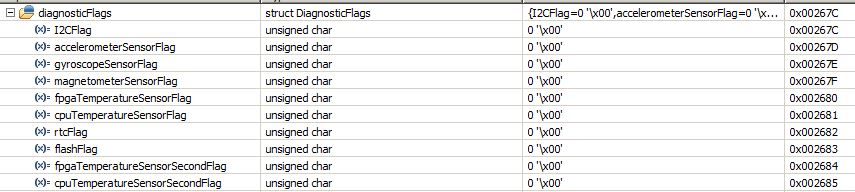
\includegraphics[scale=0.6]{examples/1_diagnosticFlagStart.JPG}}
\caption{Le flag riferite ad ogni singolo sensore è abbassata in fase di start-up del sistema}
\label{fig}
\end{figure}
\vspace{0.5cm}
Passiamo dunque al controllo del primo sensore, ovvero l'accelerometro. La funzione di controllo del sensore come prima azione alza sia la flag relativa al sensore che al bus I2C, vedi figura 5.5. Questa scelta è dovuta al fatto che il computer di bordo richiede una richiesta di comunicazione tramite un bus I2C ad un sensore che potrebbe essere rotto. A tale richiesta non corrisponderebbe mai una richiesta, creando quindi una situazione di deadlock del codice. 
In tal caso il Watchdog Timer resetterebbe il sistema e riscontrando le flag dedicate già alzate, il blocco sarebbe risolto.\newline
\begin{figure}[htbp]
\centerline{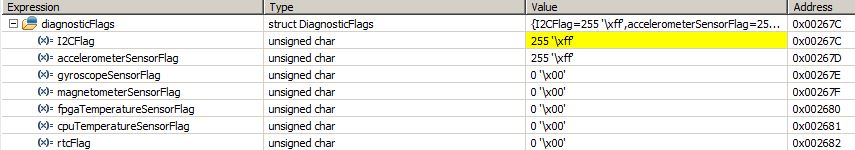
\includegraphics[scale=0.65]{examples/2_startAccelorometerCheck.JPG}}
\caption{Esclusione del sensore di accelerazione e del bus I2C in ingresso ad ogni funzione di diagnosi.}
\label{fig}
\end{figure}
\vspace{0.5cm}

Una volta ricevuta la risposta tramite bus I2C da parte dell'accelerometro, il sistema abbassa la flag relativa al funzionamento del bus I2C (vedi figura 5.6), mentre per ora la flag dell'accelerometro rimane inalterata.\newline

\begin{figure}[htbp]
\centerline{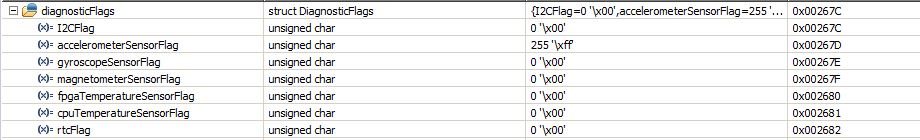
\includegraphics[scale=0.6]{examples/3_accelerometerI2CGoodConnection.JPG}}
\caption{La flag relativa al bus I2C viene abbassata dopo aver ricevuto una corretta risposta dal bus.}
\label{fig}
\end{figure}

Il prossimo controllo che la funzione di diagnosi del sensore di accelerazione esegue è il confronto tra l'ID ricevuto tramite richiesta I2C al sensore con il valore salvato a priori in memoria. Se i due valori sono coincidenti, la flag relativa all'accelerometro viene abbassata, viceversa viene lasciata alta.\newline

\begin{figure}[htbp]
\centerline{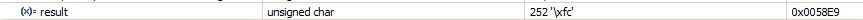
\includegraphics[scale=0.65]{examples/4_badAccelerometerId.JPG}}
\caption{Il valore di ritorno dell'ID relativo all'accelerometro.}
\label{fig}
\end{figure}

Nel nostro caso i due valori di numero identificativo relativo all'accelerometro non sono gli stessi: il valore decimale associato a priori era infatti pari a "0xE5", ovvero 229 in decimale, mentre il bus ha un valore pari a 252. L'algoritmo dunque riscontra il malfunzionamento dell'accelerometro e ritorna alla funzione generica di diagnosi dell'interno sistema con un valori di output diverso a 0 (nel nostro caso un valore pari di result pari a 1, come è evidente nella figura 5.8).\newline

\begin{figure}[htbp]
\centerline{
\includegraphics[scale=0.6]{examples/5_accelerometerCounter.JPG}}
\caption{Il valore di ritorno della funzione di diagnosi dell'accelerometro. Questo valore verrà aggiunto al valore di autodiagnosi generica.}
\label{fig}
\end{figure}

Una volta usciti dalla funzione di controllo dell'accelerometro, l'algoritmo continua con il controllo dei successivi sensori. Come è evidente dalla figura 5.9 la struttura diagnosticFlag ha mantenuto la flag relativa all'accelerometro alzata.
\newline
\begin{figure}[htbp]
\centerline{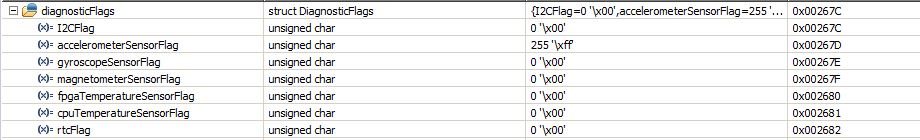
\includegraphics[scale=0.6]{examples/6_accelerometerIdBad.JPG}}
\caption{Il valore delle flag una volta superata la funzione di diagnosi dell'accelerometro.}
\label{fig}
\end{figure}

Il prossimo controllo riguarda la diagnosi dello stato del Giroscopio e del Magnetometro. Una volta superato il controllo, entrambi le funzioni ritornano un valore pari a 0 ed entrambi le flag relative ai singoli sensori rimangono abbassate (vedi figura 5.10).\newpage
\begin{figure}[htbp]
\centerline{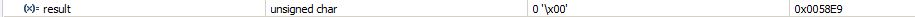
\includegraphics[scale=0.6]{examples/7_GiroscopioResultGoodI2CAndGoodMagnetometerId.JPG}}
\caption{Il valore di ritorno della funzione di diagnosi del giroscopio. Questo valore è nullo in assenza di errori o mancate risposte dal sensore e dal bus di comunicazione.}
\label{fig}
\end{figure}

Una volta ultimati tutti i controlli relativi ai sensori, l'algoritmo di autodiagnosi descrive quindi lo stato generale del sistema. La salute di tale sistema è dunque garantita dal non superamento di una soglia di rotture. Tale parametro è identificato dalla somma di tutti i valori di ritorno delle funzioni di controllo di ogni singolo sensore. Come possiamo notare nella figura 5.11 tale valore corrisponde a 1, identificando quindi la rottura del solo sensore di accelerazione.\newline
\begin{figure}[htbp]
\centerline{
\includegraphics[scale=0.6]{examples/8_giroscopioCounterRimaneAUno.JPG}}
\caption{Il valore finale di autodiagnosi responsabile di decretare la necessità di un software reset. }
\label{fig}
\end{figure}

Il valore di soglia viene confrontato con la soglia di "0x8". Se il valore di counter è superiore a tale soglia, il sistema viene riavviato. Nel nostro caso (vedi figura 5.12), il controllo ha esito negativo e dunque il sistema continua la sua inizializzazione e terminando l'algoritmo di autodiagnosi.\newline

\begin{figure}[htbp]
\centerline{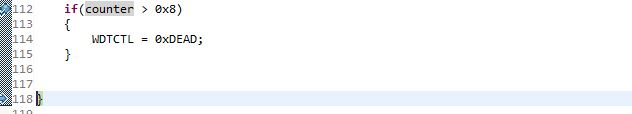
\includegraphics[scale=0.7]{examples/9_ControlloDelNumeroDiFaultNO_RIAVVIO.JPG}}
\caption{Controllo di superamento della soglia di riavvio del sistema.}
\label{fig}
\end{figure}


\newpage





\chapter{Algoritmo di controllo del raggiungimento dell' orbita}
Il compito principale di questo algoritmo consiste dunque nella valutazione del modulo dell’accelerazione del satellite. Questa parte di codice è relativa alla fase di inizializzazione del sistema e viene disattivata tramite un' apposita flag una volta utilizzata per la prima volta, in modo da garantire la non generazione di una "deadlock" del sistema, ovvero un ciclo continuo di reset e utilizzo di questa funzione il quale potrebbe compromettere l'inizio della missione.

\section{Descrizione del sensore di accelerazione ADXL-345}
\begin{figure}[htbp]
\centerline{\includegraphics[scale=0.5]{examples/AbacusAccelerometer.PNG}}
\caption{Orientamento dei sensori accelerometro e magnetometro}
\label{fig}
\end{figure}
\vspace{0.5cm}
L’accelerometro fornito da Abacus, in figura 6.1, è un dispositivo chiamato ADXL-345 della Analog Devices.
Le caratteristiche principali di questo dispositivo sono:
\begin{itemize}
    \item Misurazione su tre assi (x,y,z)
     
    \item Range di misura selezionabile a 2g,4g,8g,16g
    
    \item Risoluzione: fisso a 10 bit, nel caso di modalità a massima risoluzione arriva a 13 bit a          +16g (mantenendo 4 mg/LSB come fattore di scala) 
    
    \item Sensibility: 256 LSB/g, 128LSB/g, 64LSG/g, 32LSB/g

     \item Alimentazione da 2.0 V  a 3.6 V

     \item I/0 voltage range: 1.7 V a $V_s$

     \item Protocollo di comunicazione: SPI ( 3 o 4-wire) e $I^2C$ digital interface

     \item Consumi: $23 /mu A$ in measurement mode, $0.1 /mu A$ in standby mode con una $V_s = 2.5V$

     \item Dimensioni: 3mm x 5mm x 1mm LGA package
\end{itemize}



\section{Circular Buffer}
\begin{figure}[htbp]
\centerline{\includegraphics[scale=0.5]{examples/CircularBuffer.PNG}}
\caption{Rappresentazione grafica di un buffer circolare.}
\label{fig}
\end{figure}
\newline
Il circular buffer o anche chiamato cyclic buffer è uno spazio di memoria di dimensioni fissa che permette di immagazzinare per un periodo illimitato di volte un determinato valore in ingresso.

L'implementazione è molto semplice e comprende:
\begin{itemize}
    \item Un semplice buffer a grandezza definita;
    
    \item Un indice per capire quale elemento è stato scritto per ultimo. Questo valore viene normalmente viene incrementato ad ogni scrittura del buffer o resettato a zero nel caso si sia arrivati al limite del buffer;
\end{itemize}

\newline

Analizziamo dunque il codice C riguardante la struttura "Circular Buffer" utilizzata in questo caso per calcolare l'accelerazione media:

\begin{lstlisting}[language=C]
typedef struct CircularBuffer
{
    int32_t buffer[ACCELERATION_BUFFER_SIZE];
    int32_t mean3DAcceleration;
    uint8_t index;
}CircularBuffer;

CircularBuffer accelerationBuffer;
\end{lstlisting}

\section{Struttura del codice di controllo dell'accelerazione}
Come abbiamo prima spiegato, l'accelerometro è dunque un sensore triassiale. Questo significa che  le misurazioni sono rispettivamente dell'accelerazione secondo l'asse x,y e z.

Il nostro obiettivo è campionareil valore medio del modulo dell’accelerazione. Per avere tale valore, è necessario prima elaborare i dati forniti e poi eseguire una media dei valori calcolati. 

L’algoritmo infine valuta l’accelerazione del satellite e la confronta con un valore di soglia massima (essendo la misura di modulo un valore necessariamente non negativo).
In questo modo è possibile valutare l’effettivo raggiungimento dell’orbita determinata dalla diminuzione dell’accelerazione terrestre a cui il satellite è soggetto. Questo valore di accelerazione critico è stato dunque definito come la metà dell'accelerazione di gravità.

Nel caso in cui all’accensione del satellite si verificasse la misurazione di una accelerazione sopra la soglia decisa, l'algoritmo obbligherebbe il microcontrollore a non fare operazioni ed aspettare per un tempo limitato. Questo blocco è mirato sia a limitare i consumi (dato che il satellite non potrebbe ricaricare le proprie batterie quando ancora non è in orbita), sia a evitare la repentina accensione di tutte le operazioni programmate ad avvenire dopo il raggiungimento dell’ orbita in cui la missione dovrebbe svolgersi. 

Questo controllo è unico, ovvero viene eseguito soltanto all’accensione e soltanto una volta (non periodicamente dunque). In questo modo viene garantita la sicura partenza della missione e permette di assicurarci una possibile inattività perenne del sistema.

Poiché il campionamento dell’accelerazione da parte del sensore è soggetto a degli errori di misurazione e ad una incertezza definita nel datasheet dello stesso dispositivo, l’algoritmo fa uso di una valutazione dell’accelerazione media per un numero di campionamenti definiti a priori (nel nostro caso 64 campioni, ovvero la grandezza del buffer).
In questo modo è possibile mitigare l’effetto di eventuali errori di misurazione del satellite.

Per mantenere traccia degli ultimi N campioni di accelerazione è necessario dunque implementare un “Circular Buffer”.

Una volta ultimata la scrittura della zona di memoria, l’algoritmo riconosce l’eventuale sforamento della zona di memoria e conseguentemente riparte dall’indice iniziale (ovvero la prima locazione del buffer) e conseguentemente tende a sovrascrivere il valore più vecchio salvato.

L’unica accortezza che il programmatore deve mantenere è quella di aspettare un periodo di tempo minimo prima di eseguire una misura di accelerazione media poiché la zona di memoria che inizialmente è ancora non scritta e Persistent ha dei valori di accelerazioni non coerenti.

La formula del calcolo del modulo quadro dei valori medi di accelerazione del satellite:

\begin{equation}
    |A| = \sqrt{\floor{\frac{\sum_{k=0}^N (a_x^2+a_y^2+a_z^2) }{N} } }
\end{equation}

\section{Test dell'algoritmo di controllo di raggiungimento dell'orbita}

In questa sezione è stato analizzato l'algoritmo di raggiungimento dell'orbita, simulando una situazione realistica di utilizzo.

Il codice è stato dunque testato tramite un main di test in cui sono state utilizzate tutte le funzioni necessarie per calcolare il valore medio di accelerazione.

I valori di input utilizzati per il test sono una serie di campioni generati casualmente.

Il codice di test è stato compilato utilizzando un compilatore gcc 9.7.0, ovvero la versione ad oggi più aggiornata, ma è replicabile anche con versioni precedenti di compilatore gcc o altri compilatori ed utilizza unicamente librerie standard.

L'obiettivo finale di questo test è stato quello di valutare la correttezza del codice eseguito, ponendoci da oracolo e valutando tramite l'osservazione diretta la correttezza dell'algoritmo di raggiungimento dell'orbita.

La formula che stima la correttezza del codice è:

\begin{equation}
     C_{\% codice}  = 1 - \Delta_{\% errore} = 1 - \sum_{k=0}^{N} | y_{corretto} - y_{osservato} |
\end{equation}

A prescindere dalla modalità di test, i requisiti che il sistema dovrà garantire durante l'esecuzione del codice saranno:
\begin{itemize}
    \item Salvataggio di ogni singolo campione all'interno del Circular Buffer.
    
    \item Calcolo della media dei valori immagazzinati.
\end{itemize}


\subsection{Codice sorgente dell'algoritmo di controllo del raggiungimento dell'orbita}

Acceleration.h:
\begin{small}
\begin{lstlisting}[language=C]
#ifndef ACCELERATION_H_
#define ACCELERATION_H_

//il valore (modulo quadro) massimo da confrontare con il valore corrente di accelerazione (servirà un valore molto più basso)
#define THRESHOLD_ACCELERATION 5 // [ m^2*sec^-4 ]
#define ACCELERATION_BUFFER_SIZE 32
#include "abacus.h"
//uint32_t PrevTime=RTC_abacus_millis();

/*
 *
 * Function to set acceleration in the buffer AccelerationBuffer
 *
 */
void addAcceleration(const int32_t* a);
/*
 *
 * Function to set absolute value of acceleration 
 *
 */
void setAbsAcceleration();
/*
 *
 * Function to get absolute value of acceleration
 *
 */
int32_t getAbsAcceleration();
/*
 *
 * Function to get the mean value of acceleration (mean between ACCELEARTION_BUFFER_SIZE amount of samples)
 *
 */
int32_t getMeanAcceleration();
/*
 *
 * Function to check if satellite has acceleration while code is running. This should check only one time acceleration and stop all the operations if needed for N seconds
 *
 */
uint8_t checkAccelerationAtStartTime();

typedef struct CircularBuffer
{
float buffer[ACCELERATION_BUFFER_SIZE];
float mean3DAcceleration;
uint8_t index;
uint8_t full;
}CircularBuffer;

CircularBuffer accelerationBuffer;

uint8_t isSatelliteInSpace();

#endif
\end{lstlisting}
\end{small}
Acceleration.c:
\begin{small}
\begin{lstlisting}[language=C]
#include "Acceleration.h"
#include <math.h>
#include "abacus.h"

void addAcceleration(const int32_t* a)
{
    accelerationBuffer.buffer[accelerationBuffer.index % ACCELERATION_BUFFER_SIZE] = *a;

    if(accelerationBuffer.index < ACCELERATION_BUFFER_SIZE){
        ++accelerationBuffer.index;
    }else{
        accelerationBuffer.index=0;
    }

    if(!accelerationBuffer.full && ( accelerationBuffer.index == ACCELERATION_BUFFER_SIZE ) ){
        accelerationBuffer.full = 0xff;
    }
    accelerationBuffer.mean3DAcceleration = getMeanAcceleration();

}

void setAbsAcceleration()
{
    int32_t absAccelerationValue=getAbsAcceleration();
    addAcceleration(&absAccelerationValue);
}

int32_t getAbsAcceleration()
{

    int16_t x, y, z;
    float xFloat, yFloat, zFloat;   
    //This constant value is a multiplier needed to evaluate acceleration on earth
    float earthAccelerationMultiplier = 0.04f;
    int32_t result;

    abacus_sensors_acc_read(&x, &y, &z);
    //This conversion front int16_t to float is needed to evaluate with more precision the absolute value of acceleration
    xFloat = (float)(x) * earthAccelerationMultiplier;
    yFloat = (float)(y) * earthAccelerationMultiplier;
    zFloat = (float)(z) * earthAccelerationMultiplier;
    result = (int32_t) floor( sqrt(xFloat * xFloat + yFloat * yFloat + zFloat * zFloat ) ) ;
    return result;
}

int32_t getMeanAcceleration()
{
    int32_t result=0;
    short i;
    if(accelerationBuffer.full == 0x0 ){

        for (i=0;i<accelerationBuffer.index;++i){
            result+=accelerationBuffer.buffer[i];
        }

        result = result/accelerationBuffer.index;
    }
    else{

        for (i=0;i<ACCELERATION_BUFFER_SIZE;++i){
            result+=accelerationBuffer.buffer[i];
        }

        result = result/ACCELERATION_BUFFER_SIZE;
    }
    return result;
}

uint8_t checkAccelerationAtStartTime()
{

    if(getMeanAcceleration()>THRESHOLD_ACCELERATION){

        return 0xff;
    }
    else
    {
        return 0;
    }
}

uint8_t isSatelliteInSpace()
{
    uint8_t result=0x0;
    uint16_t i;
    for( i=2*ACCELERATION_BUFFER_SIZE;i>0; --i){
        setAbsAcceleration();
        //blink_routine(100);

    }
    if(!checkAccelerationAtStartTime())
    {
        abacus_sleep_msec(100000UL); //number of msecseconds = 100 sec
        result=0xff;
    }
    return result;
}

\end{lstlisting}
\end{small}
\subsection{Test comparativo per il calcolo del valore medio tramite il Circular Buffer}

Data la semplicità del componente software, il test di funzionamento è stato eseguito tramite compilatore gcc e direttamente da terminale Linux. La scelta è stata possibile poiché il suo test non necessita di nessuna libreria esterna.

Il test è consistito nella creazione della zona di memoria \textbf{"accelerationBuffer"}, inizialmente vuota e quindi inizializzata con i valori di default.

Il main, ovvero la funzione principale del codice di test, si è occupato di stimolare le funzioni utilizzate per popolare il buffer circolare e per estrarre il valore medio dei campioni contenuti in memoria.

La tipologia di test utilizzata per appurare la correttezza delle funzioni utilizzate è definita "Comparison Test", ovvero un test comparativo tra il codice da testare e un codice già esistente.

Per eseguire questa tipologia di test è necessario utilizzare gli stessi valori di input e a posteriori valutare i valori forniti in output. Per valutare tutte le proprietà del buffer circolare è inoltre necessario inserire un numero di campioni superiori alla grandezza del buffer. In questo modo il buffer dovrebbe "risaltare" all'inizio della zona di memoria e quindi sovrascrivere i valori più vecchi di accelerazione. In questo modo è possibile valutare il comportamento dell'algoritmo durante la fase più critica di esecuzione.

Per quanto riguarda gli input fornito all'algoritmo sono stati generati tre diversi valori di accelerazione ad ogni singola iterazione, questo perchè l'accelerometro è uno sensore che valuta campioni sui tre diversi assi (x,y,z).
Ogni singola tripletta di campioni di accelerazione viene quindi trasformata in un valore medio di accelerazione e successivamente salvato nella memoria del buffer.

I valori di accelerazione media sono dunque stati salvati in un file ".csv" in entrambe i due test (sia del nostro codice che di quello ritenuto corretto).

Di seguito è disponibile il file main.c utilizzato per testare il componente:

\begin{small}
\begin{lstlisting}[language=C]
#include <stdio.h>
#include "Acceleration.h"
#include <time.h>

int main()
{
    
    srand(time(NULL));
    unsigned short i = 0;
    int x,y,z;
    
    FILE *fs;
    fs = fopen("result.csv", "a");	//Creazione del file .csv in cui salvare i valori di accelerazione e 
					//relativo valore calcolato di accelerazione media
	if(fs == NULL){
	    printf("Couldn't open file\n");
	    return;
	}
	fprintf(fs, "X,Y,Z,mean\n");	//L'header del formato csv
    fclose(fs);
	
    for (i = 0; i < 3*ACCELERATION_BUFFER_SIZE ;++i){
	
    	x = 25*7-(2*rand()%2-1)*(rand()%5)-2*i;
    	y = (2*rand()%2-1)*(rand()%15);
    	z = 40+(2*rand()%2-1)*(rand()%5);
        int a = getAbsAcceleration(x,y,z);
        addAcceleration(&a);
    }    
	
	

    unsigned char satelliteStatus = isSatelliteInSpace();
    if(satelliteStatus!=0){
        printf("\nSoglia non superata\n");
    }else{
        printf("\nSoglia SUPERATA\n");
    }

    return 0;
}
\end{lstlisting}
\end{small}

Anche  l'implementazione di alcune funzioni in Acceleration.c sono state modificate per poter iniettare degli input arbitrari.
\newline
Modifiche a Acceleration.c:
\begin{lstlisting}[language=C]
int32_t getAbsAcceleration(int32_t x, int32_t y, int32_t z)
{
    
    FILE *fs;
    fs = fopen("result.csv", "a");

    float xFloat, yFloat, zFloat;   
    //This constant value is a multiplier needed to evaluate acceleration on earth
    float earthAccelerationMultiplier = 0.04f;
    int32_t result;

    //abacus_sensors_acc_read(&x, &y, &z);
    //This conversion front int16_t to float is needed to evaluate with more precision the absolute value of acceleration
    xFloat = (float)(x) * earthAccelerationMultiplier;
    yFloat = (float)(y) * earthAccelerationMultiplier;
    zFloat = (float)(z) * earthAccelerationMultiplier;
    result = (int32_t) floor( sqrt(xFloat * xFloat + yFloat * yFloat + zFloat * zFloat ) ) ;
    fprintf(fs, "%f,%f,%f,",xFloat,yFloat,zFloat);

    fclose(fs);
    return result;
}
\end{lstlisting}

\subsection{Confronto dei risultati dei test con implementazione di libreria boost}

In questa sezione l'obiettivo è stato, come abbiamo detto in precedenza, generare dei valori di uscita corretti da confrontare con i valori già precedentemente calcolati.
Per fare ciò abbiamo utilizzato un'altra implementazione di Circular Buffer di libreria ritenuta quindi senza bug e dunque corretto. Il nostro compito è stato generare un main che a partire dagli stessi input generasse degli output attraverso le stesse operazioni matematiche.

La libreria utilizzata è chiamata \textbf{"Boost"}, una libreria di codice per il linguaggio di programmazione C++.

I valori calcolati sono poi salvati in una file ".csv", come nell'algoritmo di test del nostro algoritmo di raggiungimento dell'orbita.
\newline\newline
Di seguito è possibile consultare il main della versione di confronto in linguaggio C++:
\newline
\begin{lstlisting}[language=C++]
#include <iostream>
#include <boost/circular_buffer.hpp>
#define MAX_SIZE 32
#include <math.h>
#include <vector>

std::vector<AccelerationSample> samples_;
struct AccelerationSample
{
    float x,y,z;  
};

int main(){
    
    ::boost::circular_buffer<int> myCircularBuffer_;
    myCircularBuffer_.resize(MAX_SIZE);
    
    
    FILE* fw;
    fw=fopen("resultCpp.csv","w");
    fprintf(fw,"Index,meanAcceleration\n");
    int index = 0;
    for (auto sample : samples_) {
        
        int absAcceleration = std::sqrt(sample.x*sample.x + sample.y*sample.y + sample.z*sample.z);
        myCircularBuffer_.push_back(absAcceleration); 

        
        int sizeCounter = 0;
        int meanAcceleration = 0;
         
         
        
        for (auto itr = myCircularBuffer_.begin(); itr!=myCircularBuffer_.end() ; ++itr){
              meanAcceleration+=*itr;
            if(*itr!=0){
            sizeCounter++;
            }
        }
        if(sizeCounter!=0){
            meanAcceleration = meanAcceleration/sizeCounter;
        }
        
        fprintf(fw,"%d,%d\n,",index,meanAcceleration);
        ++index;
    }
    fprintf(fw,"\n");
    fclose(fw);
    
    return 0;
}

\end{lstlisting}

\newpage
\subsection{Rappresentazione grafica dei valori di accelerazione media ottenuta in Matlab}

Per confrontare graficamente i risultati ottenuti, è stato utilizzato uno script Matlab per graficare i valori conservati nei file precedentemente generati negli script di test.

Lo script di Matlab è dunque diviso in due parti:
\begin{itemize} 
\item Nella prima parte i valori di accelerazione media (in viola) vengono confrontati con il valori di soglia di accelerazione (in verde). L'accelerazione media dopo circa 0.1 sec risulta inferiore al valore di soglia e quindi il risultato concorda con quello uscito dal codice di test C. L'obiettivo è stato valutare la correttezza sulla scelta di superamento della soglia di accelerazione media dopo un determianto periodo di tempo.
    
    \begin{figure}[htbp]
    \centerline{\includegraphics[scale=0.6]{examples/MeanAcceleration.png}}
    \caption{Grafico del confronto tra i valori di accelerazione media calcolati tramite l'algoritmo di raggiungimento dell'orbita e la soglia prefissata}
    \label{fig}
    \end{figure}
\newpage
    \item Nella seconda parte abbiamo confrontato il set di output proveniente dal codice di test con i valori calcolati con l'implementazione C++ (vedi figura 6.4). In tale immagine è possibile notare una differenza nell'output soltanto in rari casi. Questo potrebbe essere dovuto ad alcuni arrotondamenti ad intero eseguiti in modo differente dai due sistemi.

    In generale, la percentuale di errore nel confronto tra valori teorici e valori calcolati per il test eseguito è circa del 3\%, un valore accettabile specialmente per un algoritmo utilizzato una singola volta all'avvio e che dunque crea un ritardo temporale ci accensione solo alla prima accensione.
    
    \begin{figure}[htbp]
    \centerline{\includegraphics[scale=0.4]{examples/CompareAlgorithResult.png}}
    \caption{Grafico del confronto tra i valori di accelerazione media calcolati tramite l'algoritmo di raggiungimento dell'orbita e la soglia prefissata}
    \label{fig}
    \end{figure}
\end{itemize}


\newpage
Il codice Matlab main.m:
\newline
\begin{lstlisting}[language=Matlab]
clear all
clc
close all

data = readtable('result.csv');

threshold = 9.81/2;
len = size(data, 1);


mean = data.mean;
time = zeros(1,len);
for i = 1:len
    time(1,i)=1e-3 * i;
end
ax = data.X;
ay = data.Y;
az = data.Z;

plot(time,ax,'-.','LineWidth',1.5);
hold on;
plot(time,ay,'-.','LineWidth',1.5);
hold on;
plot(time,az,'-.','LineWidth',1.5);
hold on;
plot(time,mean,'LineWidth',2);
hold on;
plot(time,threshold*ones(1,len),'LineWidth',5);


xlabel('time[sec]')
ylabel('Acceleration [m][sec^{-2}]')
legend('X Acceleration','Y Acceleration','Z Acceleration','Mean Acceleration','Acceleration Threshold')
grid on;
hold off;
\end{lstlisting}
\newpage
\section{Codice di prova}
Di seguito è reso disponibile il codice main utilizzato sul microcontrollore per testare tutti i nuovi componenti inseriti. 

Tutte le nuove parti di codice sono state inserite all'interno del codice originale utilizzato per Abacus. In particolare è possibile apprezzare la fase di inizializzazione del microcontrollore, ovvero la zona in cui si vanno ad eseguire tutti i controlli di consistenza di memoria e dei dati più importanti. Infine vi è il controllo del raggiungimento dell'orbita, il quale non permette l'accensione accidentale del dispositivo.

Superata la fase di inizializzazione del dispositivo, si inizia con le azioni periodiche che il microcontrollore esegue. In questa fase il sistema esegue periodicamente dei controlli di integrità e nel caso di riscontro di un problema esegue un reset, permettendo di fatto il restart del dispositivo. 

Questa azione permette il controllo e l'eventuale correzione dei problemi riscontrati in fase di esecuzione del codice.
\newline\newline
Il file main.c:

\begin{small}
\begin{lstlisting}[language=C]
#include <msp430.h>
#include <stdio.h>
#include "abacus.h"
#include "bootloader/bootloader.h"
#include "satellite/satsystem_init.h"
#include "SelfDiag/selfDiag.h"
#include "SatelliteAcceleration/Acceleration.h"
#pragma CODE_SECTION(main,".text_bootloader")

/*
 * Main routine
 * After initialization the satellite checks if there are tasks to do 
 * and eventually goes to sleep.
 * If there is an interrupt that awakes the satellite the loop is executed
 * checking what has to be done before going back to sleep
 */
 
#PRAGMA PERSISTENT(satelliteInOrbitFlag)
uint8_t satelliteInOrbitFlag = 0;
int main(void)
{
    // Stop watchdog timer
    WDTCTL = WDTPW | WDTHOLD;

    //Check memory status
    int8_t bootResult = bootloaderStart();


    uint8_t scrubMemory = scrubbingRoutine();
    //Hardware initialization
    //with diagnostics
    satsystem_init();

    AB_LED_OFF;

    //Check flight status and boot into preprogrammed sequence
    bootFlightStatus();

    int8_t systemDiagnostic = selfDiagInit();


    uint8_t isSatelliteInOrbit;
    if(satelliteInOrbitFlag) {
        isSatelliteInOrbit = isSatelliteInSpace();
        satelliteInOrbitFlag = 0xff;
    }
    //Enter main loop
    while (1)
    {
        //Kick the WDT again
        WDTCTL = (WDTCTL & 0x00FF) | WDTPW | WDTCNTCL;

        checkMarie();

        //Kick the WDT again
        WDTCTL = (WDTCTL & 0x00FF) | WDTPW | WDTCNTCL;

        //Check commands on debug UART or on Radio UART
        checkRadio();

        //Kick the WDT again
        WDTCTL = (WDTCTL & 0x00FF) | WDTPW | WDTCNTCL;

        //Check commands on debug UART or on Radio UART
        checkDebugCommand();

        //Kick the WDT again
        WDTCTL = (WDTCTL & 0x00FF) | WDTPW | WDTCNTCL;

        //Check satellite status and update if necessary
        checkStatus();

        //Kick the WDT again
        WDTCTL = (WDTCTL & 0x00FF) | WDTPW | WDTCNTCL;

        //Time to do a new step of an experiment?
        checkExperiment();

        //Kick the WDT again
        WDTCTL = (WDTCTL & 0x00FF) | WDTPW | WDTCNTCL;

        //Digipeater action?
        checkRadioHam();

        //Kick the WDT again
        WDTCTL = (WDTCTL & 0x00FF) | WDTPW | WDTCNTCL;

        //Time to read telemetry?
        checkTelemetry();

        //Kick the WDT again
        WDTCTL = (WDTCTL & 0x00FF) | WDTPW | WDTCNTCL;

        //Time to send beacon?
        checkBeacon();

        //Kick the WDT again
        WDTCTL = (WDTCTL & 0x00FF) | WDTPW | WDTCNTCL;

        checkMemoryOp();

        //Kick the WDT again
        WDTCTL = (WDTCTL & 0x00FF) | WDTPW | WDTCNTCL;

        check_minute_counter();

        AB_LED_OFF;

        timer_goToSleep();

        if (satelliteConfiguration_.debugIsOn == 1)
            AB_LED_ON;
    }

    //It will never arrive here fortunately
    return 0;
}
\end{lstlisting}
\end{small}



\chapter{Conclusioni}

\section{Conclusioni sul lavoro di tesi}

Il lavoro di tesi presentato in questo elaborato si è posto l'obiettivo di progettare un sistema di controllo,protezione e correzione
utilizzato principalmente come contromisura per quanto riguarda problemi di consistenza dell'informazione contenuta in un microcontrollore contenuto all'interno di un picosatellite.

Dai risultati ottenuti attraverso l'attività di debugging e testing delle singole componenti software, è possibile affermare che l'integrità 
del sistema e la sua tolleranza rispetto ad eventuali malfunzionamenti dei singoli componenti hardware è migliorata notevolmente.

L'algoritmo di Scrubbing implementato su uno schema a blocchi di dati piccoli permette inoltre una facile scalabilità del sistema. L'algoritmo che
si occupa della rivelazione e/o della correzione di singole, doppie e addirittura triple corruzioni all'interno di
singoli blocchi ha un costo algoritmico sia temporale che spaziale di tipo lineare rispetto alla scelta del numero di blocchi che si sceglie di 
proteggere. 

Inoltre, tramite test è stato possibile evidenziare che, a parità di grandezza di memoria da proteggere, la probabilità di avere un backup integro diminuisce all'aumentare della frequenza di corruzioni che avvengono nella zona di backup nel periodo intercorso tra due scrubbing della memoria di backup.

L'utilizzo di un algoritmo di parità quadridimensionale fornisce dunque un ottimo compromesso facendo un confronto tra performance dell'algoritmo (e
quindi protezione della memoria dati) e occupazione di memoria.

Un altro sviluppo molto importante ha riguardato il controllo e la gestione di eventuali malfunzionamenti per quanto riguarda la parte di sensoristica 
e di memoria flash connessa al microcontrollore. Tale algoritmo di autodiagnosi del sistema ha fornito una semplice ma efficace strategia di diagnosi della comunicazione con un determinato sottosistema garantendo la sua continua esclusione in presenza di guasti e quindi limitando la probabilità per cui un singolo malfunzionamento generasse il blocco dell'intero sistema.

Infine l'utilizzo di un algoritmo di controllo del raggiungimento dell'orbita del satellite ha fornito un controllo aggiuntivo rispetto alla remota possibilità
di accensione non voluta del satellite. Questo evento non voluto causerebbe nel migliore dei casi uno spreco di potenza e nel peggiore dei casi la rottura del satellite
prima dell'inizio della missione.

Contando che il sistema non sia controllabile dall'esterno e quindi faccia affidamento quasi unicamente sul suo computer di bordo per poter gestire 
l'andamento della missione spaziale, il sistema ha raggiunto un grado di robustezza notevolmente maggiore rispetto a quello che aveva precedentemente, ovvero rispetto allo stesso sistema che le aveva già permesso di superare con buoni risultati diverse missioni spaziali.
\section{Possibili sviluppi futuri}
Tutto lo sviluppo software è stato implementato direttamente sul microcontrollore sprovvisto della maggior parte dei sottosistemi utilizzati durante la missione. Un possibile
sviluppo futuro potrebbe essere l'integrazione di ogni singolo componente software all'interno di un sistema completo. Tale approccio garantirebbe maggiore contezza
di eventuali criticità e miglioramenti da eseguire sul codice elaborato. 

Come ulteriore lato positivo, il testing diretto sul sistema completo garantirebbe una  minore presenza di errori e di bug di codice garantendo dunque una maggiore 
sicurezza di tutta la missione spaziale. 

Infine, questo approccio potrebbe permettere un "tuning" del sistema dal punto di vista delle  risorse software utilizzate all'interno degli algoritmi, come ad esempio la scelta del numero di copie di codice di backup che potrebbe essere inserite all'interno della memoria,
aspetto che garantirebbe sicuramente una vita del satellite notevolmente più lunga.
\chapter{Gestione di una sezione di firmware Persistent o Noinit}

\subsection{Passo 1: Dichiarazione della variabile}
Il primo passo in un codice C da compiere è dunque dichiarare la variabile voluta come uan variabile globale "Persistent" o "Noinit" (per cui la procedura è analoga). In questo modo la variabile non verrà inserita dal compilatore all'interno della sezione .bss (le variabili globali inizializzate a 0 per default) ma sarà inserita in una particolare zona di memoria indipendente che definiremo successivamente e che permetterà al microcontrollore di non inizializzare il valore ad ogni software reset che il sistema genererà periodicamente o in presenza di guasti o malfunzionamenti.


Prendiamo come esempio la dichiarazione in un semplice main:
\begin{lstlisting}[language=C]
    #pragma PERSISTENT(var)  
    unsigned long var=0;  
    SYSCFG0 = FRWPPW | DFWP;           
    var++;   
    SYSCFG0 = FRWPPW | PFWP | DFWP; 

\end{lstlisting}
\vspace{2cm}
\begin{small}
Linea 01 e 02: vanno a definire la variabile "var". La definizione \textt{#Pragma PERSISTENT(var)} dicono al compilatore di allocare la variabile "var" in una zona dedicata di memoria. L'inizializzazione di questa variabile è del tutto simile ad una definita direttamente in RAM. (Nell'esempio è posta a 0).
Si tratta dunque di un comando al "linker file" che andrà a definire in fase di linking la zona di memoria in cui allocare poi la variabile. Successivamente si occuperemo di definirlo anche nel file di linker script.\newline

Linea 03 e 05: andiamo ad esempio a definire un comando che permette la scrittura in FRAM. La scrittura viene poi disabilitata successivamente alla riga 05.\newline

Linea 04: un semplice comando di incremento. La variabile può essere dunque trattata come qualsiasi altra semplice variabile locale o globale.\newline

\end{small}


\clearpage
L'accesso ad una variabile il FRAM è totalmente analogo all'accesso alle classiche variabili site in RAM.

Lo sblocco della scrittura ed il successivo blocco è un passo totalmente opzionale anche se consigliato. L'idea è che se qualcosa di non voluto accidentalmente accade, la scrittura è ancora disabilitata e il contenuto della variabile persistent non viene alterato.

La pragma PERSISTENT permette dunque di memorizza i dati in FRAM quando il processore entra in sleep mode.
Quindi un possibile utilizzo è mettere al sicuro il contenuto delle variabili memorizzate nella RAM statica nella FRAM. (O sull'MSP430, tenerle direttamente in FRAM).

Ci sono alcuni costi di consumo energetico. Il salvataggio su FRAM richiede più energia rispetto alla RAM. Inoltre, è necessario che ci siano 10 $\mu s$ dopo l'uscita da alcune modalità di sospensione prima di poter salvare nuovamente su FRAM.

Per frequenze maggiori 8 MHz è dunque necessario inserire degli stati di "wait" dopo una scrittura in FRAM, cosa che se utilizzata in maniera sproposita può inficiare sulle prestazioni del codice.

L'unico caso in cui la variabile persistent viene inizializzata è il caso in cui il codice viene sovrascritto.
Esiste però la definizione di una variabile "noinit", la quale si comporta in maniera totalmente analoga alla persistent con
l'unica eccezione che non viene mai inizializzata.
Quello che hai a disposizione è semplicemente l'indirizzo fisso in cui la variabile è sita, nient'altro.

Vediamo un esempio di definizione di variabile globale "NOINIT":
\begin{lstlisting}[language=C]
    #pragma NOINIT(var)  
    unsigned long var;  
\end{lstlisting}

\subsection{Passo 2: Modifica alle impostazioni di Erase}
Il comando nelle impostazioni da cercare per mantenere inalterato il valore nella FRAM è il seguente:
\begin{verbatim}
    

    "Replace written memory locations" -> "Retain unwritten memory locations"
    
                                                    oppure
                                                    
                                       -> "Erase and download necessary segments 
                                            only (Differential download)"

\end{verbatim}
\subsection{Passo 3: Modifica il Linker Command File}
E' necessaria definire dunque una sezione di memoria in linker inserirà automaticamente tutte le variabili definite come ".Persistent" e come ".NoInit".

Ecco un esempio di linker script in cui è presente una sezione persistent.
Come per tutte le altre zone di memoria, è necessario definire l'inizio e la lunghezza della zona di memoria. Ricordiamo 
di creare zone di memoria non sovrapposte l'una con l'altra al fine problemi di sovrascrittura non voluta.

\begin{lstlisting}[language=C]
    lnk_msp430f5438a.cmd :
    
/****************************************************************************/
/* SPECIFY THE SYSTEM MEMORY MAP                                            */
/****************************************************************************/

MEMORY
{
    SFR                     : origin = 0x0000, length = 0x0010
    PERIPHERALS_8BIT        : origin = 0x0010, length = 0x00F0
    PERIPHERALS_16BIT       : origin = 0x0100, length = 0x0100
    RAM                     : origin = 0x1C00, length = 0x3D00	
    RAM_CODE		    : origin = 0x5900, length = 0x0300
    INFOB                   : origin = 0x1900, length = 0x0080
    INFOC                   : origin = 0x1880, length = 0x0080
    INFOD                   : origin = 0x1800, length = 0x0080
    FLASH                   : origin = 0x5C00, length = 0xA080	
    FLASH_RAM		    : origin = 0xFC80, length = 0x0300
    FLASH2                  : origin = 0x10000,length = 0xFFFF
    FLASH3                  : origin = 0x20000,length = 0xFFFF
    FLASH4                  : origin = 0x30000,length = 0xFFFF
    FLASH5                  : origin = 0x40000,length = 0x5BFF
    INT00                   : origin = 0xFF80, length = 0x0002
    INT01                   : origin = 0xFF82, length = 0x0002
    INT02                   : origin = 0xFF84, length = 0x0002
    INT03                   : origin = 0xFF86, length = 0x0002
    INT04                   : origin = 0xFF88, length = 0x0002
    INT05                   : origin = 0xFF8A, length = 0x0002
    INT06                   : origin = 0xFF8C, length = 0x0002
    INT07                   : origin = 0xFF8E, length = 0x0002
    INT08                   : origin = 0xFF90, length = 0x0002
    INT09                   : origin = 0xFF92, length = 0x0002
    INT10                   : origin = 0xFF94, length = 0x0002
    INT11                   : origin = 0xFF96, length = 0x0002
    INT12                   : origin = 0xFF98, length = 0x0002
    INT13                   : origin = 0xFF9A, length = 0x0002
    INT14                   : origin = 0xFF9C, length = 0x0002
    INT15                   : origin = 0xFF9E, length = 0x0002
    INT16                   : origin = 0xFFA0, length = 0x0002
    INT17                   : origin = 0xFFA2, length = 0x0002
    INT18                   : origin = 0xFFA4, length = 0x0002
    INT19                   : origin = 0xFFA6, length = 0x0002
    INT20                   : origin = 0xFFA8, length = 0x0002
    INT21                   : origin = 0xFFAA, length = 0x0002
    INT22                   : origin = 0xFFAC, length = 0x0002
    INT23                   : origin = 0xFFAE, length = 0x0002
    INT24                   : origin = 0xFFB0, length = 0x0002
    INT25                   : origin = 0xFFB2, length = 0x0002
    INT26                   : origin = 0xFFB4, length = 0x0002
    INT27                   : origin = 0xFFB6, length = 0x0002
    INT28                   : origin = 0xFFB8, length = 0x0002
    INT29                   : origin = 0xFFBA, length = 0x0002
    INT30                   : origin = 0xFFBC, length = 0x0002
    INT31                   : origin = 0xFFBE, length = 0x0002
    INT32                   : origin = 0xFFC0, length = 0x0002
    INT33                   : origin = 0xFFC2, length = 0x0002
    INT34                   : origin = 0xFFC4, length = 0x0002
    INT35                   : origin = 0xFFC6, length = 0x0002
    INT36                   : origin = 0xFFC8, length = 0x0002
    INT37                   : origin = 0xFFCA, length = 0x0002
    INT38                   : origin = 0xFFCC, length = 0x0002
    INT39                   : origin = 0xFFCE, length = 0x0002
    INT40                   : origin = 0xFFD0, length = 0x0002
    INT41                   : origin = 0xFFD2, length = 0x0002
    INT42                   : origin = 0xFFD4, length = 0x0002
    INT43                   : origin = 0xFFD6, length = 0x0002
    INT44                   : origin = 0xFFD8, length = 0x0002
    INT45                   : origin = 0xFFDA, length = 0x0002
    INT46                   : origin = 0xFFDC, length = 0x0002
    INT47                   : origin = 0xFFDE, length = 0x0002
    INT48                   : origin = 0xFFE0, length = 0x0002
    INT49                   : origin = 0xFFE2, length = 0x0002
    INT50                   : origin = 0xFFE4, length = 0x0002
    INT51                   : origin = 0xFFE6, length = 0x0002
    INT52                   : origin = 0xFFE8, length = 0x0002
    INT53                   : origin = 0xFFEA, length = 0x0002
    INT54                   : origin = 0xFFEC, length = 0x0002
    INT55                   : origin = 0xFFEE, length = 0x0002
    INT56                   : origin = 0xFFF0, length = 0x0002
    INT57                   : origin = 0xFFF2, length = 0x0002
    INT58                   : origin = 0xFFF4, length = 0x0002
    INT59                   : origin = 0xFFF6, length = 0x0002
    INT60                   : origin = 0xFFF8, length = 0x0002
    INT61                   : origin = 0xFFFA, length = 0x0002
    INT62                   : origin = 0xFFFC, length = 0x0002
    RESET                   : origin = 0xFFFE, length = 0x0002
}

/****************************************************************************/
/* SPECIFY THE SECTIONS ALLOCATION INTO MEMORY                              */
/****************************************************************************/

SECTIONS
{

    .bss        : {} > RAM                /* GLOBAL & STATIC VARS              */
    .TI.persistent     : {} > RAM        /* PERSISTENT added AN 3/1/2021    */
    .data       : {} > RAM
    .sysmem     : {} > RAM                /* DYNAMIC MEMORY ALLOCATION AREA    */
    .stack      : {} > RAM (HIGH)         /* SOFTWARE SYSTEM STACK             */

	.cinit      : {} > FLASH              /* INITIALIZATION TABLES             */
	.text:_isr  : {} > FLASH              /* ISR CODE SPACE                    */
    .cio        : {} > RAM                /* C I/O BUFFER                      */

    .pinit      : {} > FLASH              /* C++ CONSTRUCTOR TABLES            */
    .init_array : {} > FLASH              /* C++ CONSTRUCTOR TABLES            */
    .mspabi.exidx : {} > FLASH            /* C++ CONSTRUCTOR TABLES            */
    .mspabi.extab : {} > FLASH            /* C++ CONSTRUCTOR TABLES            */

    .text_bootloader : {} > FLASH		  /* CODE                              */
    .text_bootloaderRam: load = FLASH_RAM, run = RAM_CODE
    .text       : {} > FLASH2			  /* CODE2                             */
    .text_bankC : {} > FLASH3		      /* CODE3                             */
    .text_bankD : {} > FLASH4		      /* CODE4                             */
    .text_conf  : {} > FLASH5		  	  /* CODE5                             */
    .ram_code	:	load = FLASH_RAM	  /* Code that actually runs from RAM  */

    .const      : {} > FLASH2     		  /* CONSTANT DATA                     */

    .infoA     : {} > INFOA              /* MSP430 INFO FLASH MEMORY SEGMENTS */
    .infoB     : {} > INFOB
    .infoC     : {} > INFOC
    .infoD     : {} > INFOD



    /* MSP430 INTERRUPT VECTORS          */
    .int00       : {}               > INT00
    .int01       : {}               > INT01
    .int02       : {}               > INT02
    .int03       : {}               > INT03
    .int04       : {}               > INT04
    .int05       : {}               > INT05
    .int06       : {}               > INT06
    .int07       : {}               > INT07
    .int08       : {}               > INT08
    .int09       : {}               > INT09
    .int10       : {}               > INT10
    .int11       : {}               > INT11
    .int12       : {}               > INT12
    .int13       : {}               > INT13
    .int14       : {}               > INT14
    .int15       : {}               > INT15
    .int16       : {}               > INT16
    .int17       : {}               > INT17
    .int18       : {}               > INT18
    .int19       : {}               > INT19
    .int20       : {}               > INT20
    .int21       : {}               > INT21
    .int22       : {}               > INT22
    .int23       : {}               > INT23
    .int24       : {}               > INT24
    .int25       : {}               > INT25
    .int26       : {}               > INT26
    .int27       : {}               > INT27
    .int28       : {}               > INT28
    .int29       : {}               > INT29
    .int30       : {}               > INT30
    .int31       : {}               > INT31
    .int32       : {}               > INT32
    .int33       : {}               > INT33
    .int34       : {}               > INT34
    .int35       : {}               > INT35
    .int36       : {}               > INT36
    .int37       : {}               > INT37
    .int38       : {}               > INT38
    .int39       : {}               > INT39
    .int40       : {}               > INT40
    RTC          : { * ( .int41 ) } > INT41 type = VECT_INIT
    PORT2        : { * ( .int42 ) } > INT42 type = VECT_INIT
    USCI_B3      : { * ( .int43 ) } > INT43 type = VECT_INIT
    USCI_A3      : { * ( .int44 ) } > INT44 type = VECT_INIT
    USCI_B1      : { * ( .int45 ) } > INT45 type = VECT_INIT
    USCI_A1      : { * ( .int46 ) } > INT46 type = VECT_INIT
    PORT1        : { * ( .int47 ) } > INT47 type = VECT_INIT
    TIMER1_A1    : { * ( .int48 ) } > INT48 type = VECT_INIT
    TIMER1_A0    : { * ( .int49 ) } > INT49 type = VECT_INIT
    DMA          : { * ( .int50 ) } > INT50 type = VECT_INIT
    USCI_B2      : { * ( .int51 ) } > INT51 type = VECT_INIT
    USCI_A2      : { * ( .int52 ) } > INT52 type = VECT_INIT
    TIMER0_A1    : { * ( .int53 ) } > INT53 type = VECT_INIT
    TIMER0_A0    : { * ( .int54 ) } > INT54 type = VECT_INIT
    ADC12        : { * ( .int55 ) } > INT55 type = VECT_INIT
    USCI_B0      : { * ( .int56 ) } > INT56 type = VECT_INIT
    USCI_A0      : { * ( .int57 ) } > INT57 type = VECT_INIT
    WDT          : { * ( .int58 ) } > INT58 type = VECT_INIT
    TIMER0_B1    : { * ( .int59 ) } > INT59 type = VECT_INIT
    TIMER0_B0    : { * ( .int60 ) } > INT60 type = VECT_INIT
    UNMI         : { * ( .int61 ) } > INT61 type = VECT_INIT
    SYSNMI       : { * ( .int62 ) } > INT62 type = VECT_INIT
    .reset       : {}               > RESET  /* MSP430 RESET VECTOR         */ 
}

/****************************************************************************/
/* INCLUDE PERIPHERALS MEMORY MAP                                           */
/****************************************************************************/

-l msp430f5438a.cmd

    
\end{lstlisting}

\chapter{Progetto GitHub del codice sorgente}
E' disponibile online il progetto sia come codice sorgente che come progetto Code Composite Studio, che è gratuitamente
scaricabile e utilizzabile.

Per poter usufruire del codice è necessario aver installato uan versione di Github.

Questi sono i passi che permettono di copiare e poter utilizzare in ambiente Linux (per Windows 10 è utile scaricare MingW, strumento per windows che ci permette di sfruttare il compilatore gcc e inoltre un prompt dei comandi analogo a quello di linux).
I passi da eseguire per poter disporre del progetto e di tutti i test relativi ad ogni nuova feature sono:

\begin{itemize}
     \item Su GitHub, navigare sulla pagina principale della repository voluta.
    
    \item Creare una cartella in cui inserire il progetto da scaricare e entrarci dentro con i seguenti comandi:
    \begin{verbatim}

            $ mkdir myDirectory
            
            $ cd myDirectory
      
     
    \end{verbatim}
    \item Copiare il contenuto del progetto git nella cartella attuale:
        \begin{verbatim}
            $ git clone https://github.com/bindella1994/Thesis.git
        \end{verbatim}
\end{itemize}

Il codice è dunque organizzato per fornire diverse versioni in base alle esigenze.
Ogni versione è disponibile in un branch dedicato. Il branch principale , chiamato "main" ha con se il codice sorgente puro, ovvero un codice C con un semplice main di test del comportamento.
E' disponibile poi la versione del progetto di Code Composite Studio.

Questi sono i passi da eseguire per muoversi tramite prompt dei comandi nel branch dedicato e scaricare così la versione voluta:

\begin{itemize}
    \item Eseguiamo il fetch di tutte le versioni in modo di essere allineati con le ultime versioni

    \begin{verbatim}
        $ git fetch --all
    \end{verbatim}

     \item Facciamo lo switch di branch in modo da collocarci nella versione giusta da voler scaricare:
     
    \begin{verbatim}
        $ git checkout BRANCHNAME
        
        $ git pull origin BRANCHNAME
    \end{verbatim}
     
\end{itemize}

\chapter{Datasheet dei vari componenti utilizzati}

    \begin{table}[htbp]
    \centerline{\includegraphics[scale=.85]{examples/datasheet/abacusDatasheet7.PNG}}
    \caption{Tabella riguardante la scelta dei pinout H1 di Abacus}
    \label{fig}
    \end{table}
    
    \begin{table}[htbp]
    \centerline{\includegraphics[scale=.85]{examples/datasheet/abacusDatasheet8.PNG}}
    \caption{Tabella riguardante la scelta dei pinout H2 di Abacus}
    \label{fig}
    \end{table}
    
    \begin{table}[htbp]
    \centerline{\includegraphics[scale=.7]{examples/datasheet/abacusDatasheet2.PNG}}
    \caption{Tabella riguardante la scelta dei pinout per P1, P2, P7, JTAG1, JTAG2 e IP Pins}
    \label{fig}
    \end{table} 
    
    \begin{table}[htbp]
    \centerline{\includegraphics[scale=.7]{examples/datasheet/abacusDatasheet3.PNG}}
    \caption{Tabella riassuntiva delle caratteristiche dell'IMU 
    (magnetometro, accelerometro,  giroscopio)}
    \label{fig}
    \end{table}

    \begin{table}[htbp]
    \centerline{\includegraphics[scale=.8]{examples/datasheet/abacusDatasheet4.PNG}}
    \caption{Tabella riassuntiva dei valori limite di funzionamento di Abacus}
    \label{fig}
    \end{table}
    
    \begin{table}[htbp]
    \centerline{\includegraphics[scale=.8]{examples/datasheet/abacusDatasheet5.PNG}}
    \caption{Tabella riassuntiva dei valori consigliati di funzionamento di Abacus}
    \label{fig}
    \end{table}
    
    \begin{table}[htbp]
    \centerline{\includegraphics[scale=.8]{examples/datasheet/abacusDatasheet6.PNG}}
    \caption{Tabella riassuntiva delle caratteristiche elettriche di Abacus}
    \label{fig}
    \end{table}




\backmatter

\clearpage

\cleardoublepage
\phantomsection

%\bibliographystyle{sapthesis} % BibTeX style
%\bibliography{example/myBibliography.bib} % BibTeX database without .bib extension




\begin{thebibliography}{9}
\bibitem{Roberto Cusani} 
Prof. Roberto Cusani, Ing. Tiziano Inzerilli. 
\textit{"Teoria dell'Informazione e Codici"}. 
Edizioni Ingegneria 2000.

\bibitem{Magnus Haglund Arnesen} 
Magnus Haglund Arnesen,Christian Elias Kiær. 
\textit{"Mission Event Planning \& Error-Recovery for CubeSat Applications"}. 
Electronics System Design and Innovation, Giugno 2014.

\bibitem{Muhammad Imran} 
Muhammad Imran.
\textit{"Using COTS components in space applications"}.
Settembre 2006

\bibitem{Magne Alver Normann} 
Magne Alver Normann.
\textit{"Software Design of an Onboard Computer
for a Nanosatellite"}. 
Giugno 2016

\bibitem{Università di Trento} 
Università di Trento.
\textit{"Trasmissione Numerica" https://disi.unitn.it/~melgani/PDF/tx-num4.pdf}. 

\bibitem{Daniel Luis Pancorbo D'Ammando} 
Daniel Luis Pancorbo D'Ammando, Prof. Augusto Nascetti. 
\textit{"Progetto e realizzazione di un computer di bordo per picosatelliti basato su piattaforma ibrida microcontrollore-FPGA"}.
Anno Accademico 2010/2011

\bibitem{Github} 
Github. 
\textit{https://github.com/}


\bibitem{Abacus}
Group of Astrodynamics for the use of the Space Systems.

\textit{"GAUSS OBC ABACUS 2017 Datasheet"}

\bibitem{Texas Instruments} 
Texas Instruments. 
\textit{"MSP430F543xA, MSP430F541xA Mixed-Signal Microcontrollers datasheet"}.

\bibitem{M. J. Downey}
European Space Research and Technology Centre, Noordwijk, The Netherlands.
\textit{"Satellite Reliability"}.

\bibitem{Pier Luca Montessoro}
Prof. Pier Luca Montessoro e Luca Da Re.
\textit{"Fondamenti di Informatica – I Sistemi Embedded"}.
2007

\end{thebibliography}

\clearpage


\end{document}